\documentclass[11pt, oneside]{article}   	% use "amsart" instead of "article" for AMSLaTeX format
\usepackage{geometry}                		% See geometry.pdf to learn the layout options. There are lots.
\geometry{a4paper}                   		% ... or a4paper or a5paper or ... 
%\geometry{landscape}                		% Activate for rotated page geometry
%\usepackage[parfill]{parskip}    		% Activate to begin paragraphs with an empty line rather than an indent
\usepackage{graphicx}				% Use pdf, png, jpg, or eps§ with pdflatex; use eps in DVI mode
								% TeX will automatically convert eps --> pdf in pdflatex		
\usepackage{amssymb,amsmath}


% Tikz packages
\usepackage{float}
\usepackage{pgfplots}
\usepackage{tikz}
\usepackage{tikzsymbols}
\pgfplotsset{compat=1.15}

% Line thickness. One might want to multiply these values by 1.5 to make sure they are not too thin for printing!
\tikzset{
    ultra thin/.style= {line width=0.1pt},
    very thin/.style=  {line width=0.2pt},
    thin/.style=       {line width=0.4pt},% thin is the default line
    semithick/.style=  {line width=0.6pt},
    thick/.style=      {line width=0.8pt},
    very thick/.style= {line width=1.2pt},
    ultra thick/.style={line width=1.6pt}
}
\tikzset{every picture/.style={thin}} %or use: "`line width=1 pt,"<-- note:if you write line width, you must use a value with unit
\pgfplotsset{every axis/.append style={thin, grid style={thin,}, tick style={very thin,}}}

% Colors
\definecolor{ultikzblue}{rgb}{0.00000,0.44700,0.74100}%
\definecolor{ultikzred}{rgb}{0.85000,0.32500,0.09800}%
\definecolor{ultikzyellow}{rgb}{0.92900,0.69400,0.12500}%
\definecolor{ultikzpurple}{rgb}{0.49400,0.18400,0.55600}%
\definecolor{ultikzgreen}{rgb}{0.46600,0.67400,0.18800}%
\definecolor{ultikzburgundy}{rgb}{0.63500,0.07800,0.18400}%

\title{Ultimate TikZ Figures for Publications}
\author{Slobodan Milovanovi\'c}
%\date{}							% Activate to display a given date or no date

\begin{document}
\maketitle
%
%
%
\section{Line Plots}
Here is an example of a standard line plot with a legend.
%
\begin{figure}[H]
\centering
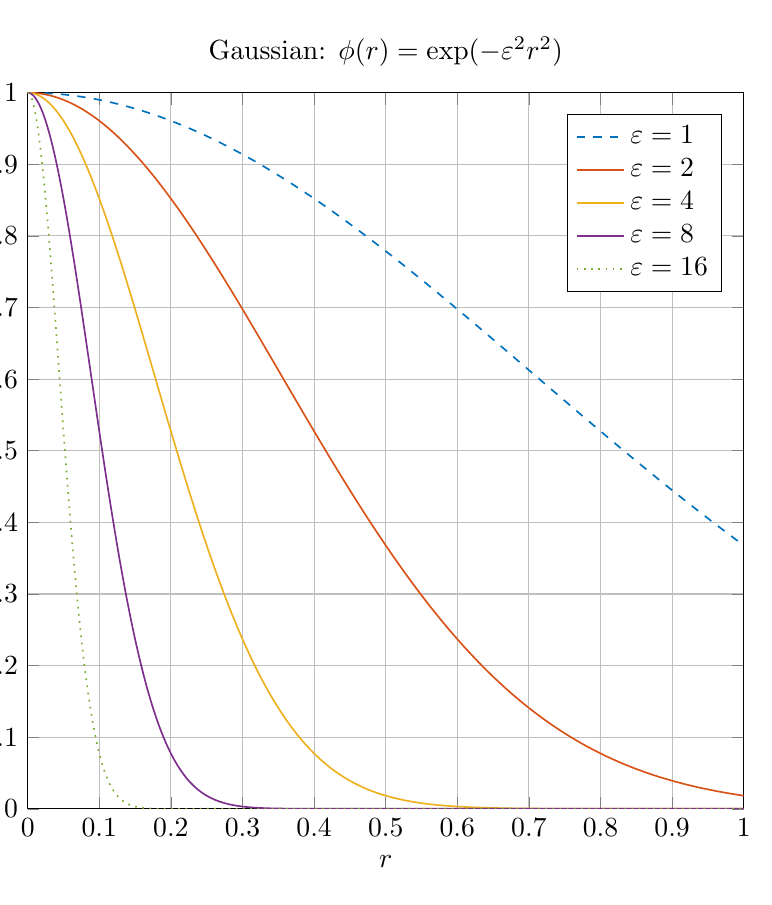
\begin{tikzpicture}[trim axis left, trim axis right, baseline]
  \begin{axis}[
  % gridlines
  grid=major,
  % dimensions
  width=0.75\textwidth, %tweak this for desired figure width on paper
  height=0.75\textwidth, %tweak this for desired figure height on paper
  at={(0\textwidth,0\textwidth)},
  scale only axis,
  unbounded coords=jump,%
% limits
  xmin=0,
  xmax=1,
  ymin=0,
  ymax=1,%
%labels
  xlabel={$r$},
  ylabel={$\phi(r)$},
  %title style={font=\bfseries},
  title={Gaussian: $\phi(r)=\exp(-\varepsilon^2 r^2)$},
%legend
  legend pos=north east,
  legend style={legend cell align=left, align=left}
  ]
\addplot [color=ultikzblue, style=dashed, semithick] %the first line, other lines are added just like this
  table[row sep=crcr]{% paste data below
  0	1\\
  0.002002002002002	0.999995991996016\\
  0.004004004004004	0.999983968080449\\
  0.00600600600600601	0.999963928542447\\
  0.00800800800800801	0.999935873863912\\
  0.01001001001001	0.999899804719482\\
  0.012012012012012	0.999855721976499\\
  0.014014014014014	0.999803626694977\\
  0.016016016016016	0.999743520127562\\
  0.018018018018018	0.999675403719478\\
  0.02002002002002	0.99959927910847\\
  0.022022022022022	0.999515148124739\\
  0.024024024024024	0.99942301279087\\
  0.026026026026026	0.999322875321747\\
  0.028028028028028	0.999214738124469\\
  0.03003003003003	0.99909860379825\\
  0.032032032032032	0.998974475134316\\
  0.034034034034034	0.998842355115795\\
  0.036036036036036	0.998702246917593\\
  0.038038038038038	0.998554153906274\\
  0.04004004004004	0.998398079639916\\
  0.042042042042042	0.998234027867976\\
  0.044044044044044	0.998062002531139\\
  0.046046046046046	0.997882007761154\\
  0.048048048048048	0.997694047880678\\
  0.0500500500500501	0.997498127403093\\
  0.0520520520520521	0.997294251032336\\
  0.0540540540540541	0.997082423662702\\
  0.0560560560560561	0.996862650378651\\
  0.0580580580580581	0.996634936454606\\
  0.0600600600600601	0.996399287354742\\
  0.0620620620620621	0.996155708732764\\
  0.0640640640640641	0.995904206431688\\
  0.0660660660660661	0.995644786483597\\
  0.0680680680680681	0.995377455109409\\
  0.0700700700700701	0.995102218718627\\
  0.0720720720720721	0.994819083909076\\
  0.0740740740740741	0.994528057466649\\
  0.0760760760760761	0.994229146365028\\
  0.0780780780780781	0.993922357765412\\
  0.0800800800800801	0.993607699016224\\
  0.0820820820820821	0.993285177652825\\
  0.0840840840840841	0.992954801397209\\
  0.0860860860860861	0.992616578157693\\
  0.0880880880880881	0.992270516028608\\
  0.0900900900900901	0.99191662328997\\
  0.0920920920920921	0.991554908407152\\
  0.0940940940940941	0.991185380030548\\
  0.0960960960960961	0.990808046995225\\
  0.0980980980980981	0.990422918320575\\
  0.1001001001001	0.99003000320995\\
  0.102102102102102	0.989629311050304\\
  0.104104104104104	0.989220851411808\\
  0.106106106106106	0.988804634047481\\
  0.108108108108108	0.988380668892793\\
  0.11011011011011	0.987948966065272\\
  0.112112112112112	0.987509535864105\\
  0.114114114114114	0.987062388769724\\
  0.116116116116116	0.986607535443393\\
  0.118118118118118	0.98614498672678\\
  0.12012012012012	0.985674753641531\\
  0.122122122122122	0.985196847388831\\
  0.124124124124124	0.984711279348956\\
  0.126126126126126	0.984218061080826\\
  0.128128128128128	0.983717204321545\\
  0.13013013013013	0.983208720985933\\
  0.132132132132132	0.982692623166056\\
  0.134134134134134	0.982168923130746\\
  0.136136136136136	0.981637633325118\\
  0.138138138138138	0.981098766370071\\
  0.14014014014014	0.980552335061792\\
  0.142142142142142	0.979998352371252\\
  0.144144144144144	0.979436831443688\\
  0.146146146146146	0.978867785598085\\
  0.148148148148148	0.97829122832665\\
  0.15015015015015	0.977707173294281\\
  0.152152152152152	0.977115634338022\\
  0.154154154154154	0.976516625466521\\
  0.156156156156156	0.975910160859477\\
  0.158158158158158	0.975296254867076\\
  0.16016016016016	0.974674922009433\\
  0.162162162162162	0.974046176976012\\
  0.164164164164164	0.973410034625051\\
  0.166166166166166	0.972766509982977\\
  0.168168168168168	0.972115618243815\\
  0.17017017017017	0.971457374768587\\
  0.172172172172172	0.970791795084711\\
  0.174174174174174	0.970118894885389\\
  0.176176176176176	0.969438690028991\\
  0.178178178178178	0.968751196538434\\
  0.18018018018018	0.96805643060055\\
  0.182182182182182	0.96735440856545\\
  0.184184184184184	0.966645146945889\\
  0.186186186186186	0.965928662416612\\
  0.188188188188188	0.965204971813704\\
  0.19019019019019	0.964474092133932\\
  0.192192192192192	0.963736040534077\\
  0.194194194194194	0.962990834330263\\
  0.196196196196196	0.962238490997283\\
  0.198198198198198	0.961479028167913\\
  0.2002002002002	0.960712463632226\\
  0.202202202202202	0.959938815336897\\
  0.204204204204204	0.9591581013845\\
  0.206206206206206	0.958370340032806\\
  0.208208208208208	0.957575549694071\\
  0.21021021021021	0.956773748934317\\
  0.212212212212212	0.955964956472611\\
  0.214214214214214	0.955149191180338\\
  0.216216216216216	0.954326472080464\\
  0.218218218218218	0.953496818346799\\
  0.22022022022022	0.952660249303254\\
  0.222222222222222	0.951816784423089\\
  0.224224224224224	0.950966443328158\\
  0.226226226226226	0.95010924578815\\
  0.228228228228228	0.949245211719822\\
  0.23023023023023	0.948374361186227\\
  0.232232232232232	0.947496714395942\\
  0.234234234234234	0.946612291702283\\
  0.236236236236236	0.945721113602521\\
  0.238238238238238	0.944823200737087\\
  0.24024024024024	0.943918573888782\\
  0.242242242242242	0.943007253981969\\
  0.244244244244244	0.942089262081774\\
  0.246246246246246	0.941164619393267\\
  0.248248248248248	0.940233347260654\\
  0.25025025025025	0.939295467166448\\
  0.252252252252252	0.938351000730654\\
  0.254254254254254	0.93739996970993\\
  0.256256256256256	0.936442395996754\\
  0.258258258258258	0.935478301618592\\
  0.26026026026026	0.934507708737042\\
  0.262262262262262	0.933530639646998\\
  0.264264264264264	0.932547116775787\\
  0.266266266266266	0.93155716268232\\
  0.268268268268268	0.930560800056224\\
  0.27027027027027	0.92955805171698\\
  0.272272272272272	0.928548940613052\\
  0.274274274274274	0.927533489821011\\
  0.276276276276276	0.926511722544659\\
  0.278278278278278	0.925483662114144\\
  0.28028028028028	0.924449331985075\\
  0.282282282282282	0.923408755737629\\
  0.284284284284284	0.922361957075658\\
  0.286286286286286	0.92130895982579\\
  0.288288288288288	0.920249787936524\\
  0.29029029029029	0.919184465477328\\
  0.292292292292292	0.918113016637725\\
  0.294294294294294	0.917035465726377\\
  0.296296296296296	0.915951837170173\\
  0.298298298298298	0.914862155513303\\
  0.3003003003003	0.913766445416335\\
  0.302302302302302	0.912664731655285\\
  0.304304304304304	0.911557039120684\\
  0.306306306306306	0.910443392816647\\
  0.308308308308308	0.909323817859926\\
  0.31031031031031	0.908198339478977\\
  0.312312312312312	0.907066983013005\\
  0.314314314314314	0.905929773911021\\
  0.316316316316316	0.904786737730889\\
  0.318318318318318	0.903637900138368\\
  0.32032032032032	0.902483286906156\\
  0.322322322322322	0.901322923912926\\
  0.324324324324324	0.900156837142364\\
  0.326326326326326	0.898985052682199\\
  0.328328328328328	0.897807596723234\\
  0.33033033033033	0.896624495558373\\
  0.332332332332332	0.895435775581642\\
  0.334334334334334	0.894241463287214\\
  0.336336336336336	0.893041585268424\\
  0.338338338338338	0.891836168216785\\
  0.34034034034034	0.890625238921003\\
  0.342342342342342	0.889408824265987\\
  0.344344344344344	0.888186951231853\\
  0.346346346346346	0.886959646892937\\
  0.348348348348348	0.88572693841679\\
  0.35035035035035	0.884488853063185\\
  0.352352352352352	0.88324541818311\\
  0.354354354354354	0.88199666121777\\
  0.356356356356356	0.880742609697576\\
  0.358358358358358	0.879483291241139\\
  0.36036036036036	0.878218733554258\\
  0.362362362362362	0.876948964428911\\
  0.364364364364364	0.875674011742238\\
  0.366366366366366	0.874393903455524\\
  0.368368368368368	0.873108667613182\\
  0.37037037037037	0.871818332341735\\
  0.372372372372372	0.870522925848789\\
  0.374374374374374	0.869222476422014\\
  0.376376376376376	0.867917012428118\\
  0.378378378378378	0.866606562311816\\
  0.38038038038038	0.865291154594808\\
  0.382382382382382	0.863970817874743\\
  0.384384384384384	0.862645580824192\\
  0.386386386386386	0.861315472189611\\
  0.388388388388388	0.85998052079031\\
  0.39039039039039	0.858640755517417\\
  0.392392392392392	0.857296205332837\\
  0.394394394394394	0.855946899268219\\
  0.396396396396396	0.854592866423914\\
  0.398398398398398	0.853234135967937\\
  0.4004004004004	0.851870737134919\\
  0.402402402402402	0.850502699225073\\
  0.404404404404404	0.849130051603145\\
  0.406406406406406	0.847752823697371\\
  0.408408408408408	0.846371044998432\\
  0.41041041041041	0.844984745058407\\
  0.412412412412412	0.843593953489727\\
  0.414414414414414	0.842198699964128\\
  0.416416416416416	0.840799014211601\\
  0.418418418418418	0.839394926019345\\
  0.42042042042042	0.837986465230716\\
  0.422422422422422	0.836573661744177\\
  0.424424424424424	0.835156545512252\\
  0.426426426426426	0.833735146540469\\
  0.428428428428428	0.832309494886311\\
  0.43043043043043	0.830879620658169\\
  0.432432432432432	0.829445554014283\\
  0.434434434434434	0.828007325161697\\
  0.436436436436436	0.826564964355201\\
  0.438438438438438	0.825118501896286\\
  0.44044044044044	0.823667968132084\\
  0.442442442442442	0.822213393454322\\
  0.444444444444444	0.820754808298268\\
  0.446446446446446	0.819292243141678\\
  0.448448448448448	0.817825728503745\\
  0.45045045045045	0.81635529494405\\
  0.452452452452452	0.814880973061504\\
  0.454454454454454	0.813402793493306\\
  0.456456456456456	0.811920786913886\\
  0.458458458458458	0.810434984033856\\
  0.46046046046046	0.808945415598962\\
  0.462462462462462	0.807452112389032\\
  0.464464464464464	0.805955105216931\\
  0.466466466466466	0.804454424927511\\
  0.468468468468468	0.802950102396562\\
  0.47047047047047	0.801442168529768\\
  0.472472472472472	0.79993065426166\\
  0.474474474474474	0.79841559055457\\
  0.476476476476476	0.796897008397589\\
  0.478478478478478	0.795374938805521\\
  0.48048048048048	0.793849412817842\\
  0.482482482482482	0.792320461497659\\
  0.484484484484485	0.790788115930669\\
  0.486486486486487	0.789252407224118\\
  0.488488488488488	0.787713366505768\\
  0.49049049049049	0.786171024922853\\
  0.492492492492492	0.78462541364105\\
  0.494494494494495	0.783076563843438\\
  0.496496496496497	0.781524506729473\\
  0.498498498498498	0.779969273513948\\
  0.500500500500501	0.778410895425968\\
  0.502502502502503	0.776849403707919\\
  0.504504504504504	0.775284829614443\\
  0.506506506506507	0.773717204411409\\
  0.508508508508508	0.77214655937489\\
  0.510510510510511	0.770572925790143\\
  0.512512512512513	0.768996334950585\\
  0.514514514514514	0.767416818156776\\
  0.516516516516517	0.7658344067154\\
  0.518518518518518	0.764249131938253\\
  0.520520520520521	0.762661025141225\\
  0.522522522522523	0.761070117643292\\
  0.524524524524524	0.759476440765504\\
  0.526526526526527	0.757880025829981\\
  0.528528528528528	0.756280904158901\\
  0.530530530530531	0.754679107073505\\
  0.532532532532533	0.75307466589309\\
  0.534534534534535	0.75146761193401\\
  0.536536536536537	0.749857976508682\\
  0.538538538538539	0.74824579092459\\
  0.540540540540541	0.746631086483293\\
  0.542542542542543	0.745013894479435\\
  0.544544544544545	0.743394246199757\\
  0.546546546546547	0.741772172922114\\
  0.548548548548549	0.74014770591449\\
  0.550550550550551	0.73852087643402\\
  0.552552552552553	0.736891715726011\\
  0.554554554554555	0.735260255022971\\
  0.556556556556557	0.733626525543629\\
  0.558558558558559	0.731990558491975\\
  0.560560560560561	0.730352385056288\\
  0.562562562562563	0.728712036408173\\
  0.564564564564565	0.727069543701598\\
  0.566566566566567	0.725424938071941\\
  0.568568568568569	0.723778250635031\\
  0.570570570570571	0.722129512486194\\
  0.572572572572573	0.720478754699309\\
  0.574574574574575	0.718826008325857\\
  0.576576576576577	0.717171304393979\\
  0.578578578578579	0.715514673907537\\
  0.580580580580581	0.713856147845175\\
  0.582582582582583	0.712195757159386\\
  0.584584584584585	0.710533532775583\\
  0.586586586586587	0.708869505591169\\
  0.588588588588589	0.707203706474613\\
  0.590590590590591	0.705536166264531\\
  0.592592592592593	0.703866915768767\\
  0.594594594594595	0.702195985763479\\
  0.596596596596597	0.70052340699223\\
  0.598598598598599	0.698849210165079\\
  0.600600600600601	0.697173425957677\\
  0.602602602602603	0.695496085010367\\
  0.604604604604605	0.69381721792729\\
  0.606606606606607	0.692136855275489\\
  0.608608608608609	0.690455027584021\\
  0.610610610610611	0.68877176534307\\
  0.612612612612613	0.687087099003067\\
  0.614614614614615	0.685401058973809\\
  0.616616616616617	0.683713675623589\\
  0.618618618618619	0.68202497927832\\
  0.620620620620621	0.680335000220672\\
  0.622622622622623	0.678643768689208\\
  0.624624624624625	0.676951314877522\\
  0.626626626626627	0.67525766893339\\
  0.628628628628629	0.673562860957914\\
  0.630630630630631	0.671866921004675\\
  0.632632632632633	0.670169879078892\\
  0.634634634634635	0.668471765136582\\
  0.636636636636637	0.666772609083725\\
  0.638638638638639	0.665072440775433\\
  0.640640640640641	0.663371290015122\\
  0.642642642642643	0.661669186553692\\
  0.644644644644645	0.659966160088706\\
  0.646646646646647	0.658262240263578\\
  0.648648648648649	0.656557456666763\\
  0.650650650650651	0.654851838830949\\
  0.652652652652653	0.653145416232258\\
  0.654654654654655	0.651438218289449\\
  0.656656656656657	0.649730274363123\\
  0.658658658658659	0.648021613754938\\
  0.660660660660661	0.646312265706825\\
  0.662662662662663	0.644602259400205\\
  0.664664664664665	0.642891623955219\\
  0.666666666666667	0.641180388429955\\
  0.668668668668669	0.63946858181968\\
  0.670670670670671	0.637756233056085\\
  0.672672672672673	0.636043371006523\\
  0.674674674674675	0.634330024473259\\
  0.676676676676677	0.632616222192721\\
  0.678678678678679	0.63090199283476\\
  0.680680680680681	0.62918736500191\\
  0.682682682682683	0.627472367228652\\
  0.684684684684685	0.625757027980692\\
  0.686686686686687	0.624041375654231\\
  0.688688688688689	0.622325438575247\\
  0.690690690690691	0.620609244998783\\
  0.692692692692693	0.618892823108233\\
  0.694694694694695	0.617176201014643\\
  0.696696696696697	0.615459406756007\\
  0.698698698698699	0.613742468296569\\
  0.700700700700701	0.612025413526142\\
  0.702702702702703	0.610308270259412\\
  0.704704704704705	0.608591066235266\\
  0.706706706706707	0.606873829116112\\
  0.708708708708709	0.605156586487208\\
  0.710710710710711	0.603439365856001\\
  0.712712712712713	0.601722194651462\\
  0.714714714714715	0.60000510022343\\
  0.716716716716717	0.598288109841966\\
  0.718718718718719	0.596571250696703\\
  0.720720720720721	0.59485454989621\\
  0.722722722722723	0.593138034467352\\
  0.724724724724725	0.591421731354662\\
  0.726726726726727	0.589705667419717\\
  0.728728728728729	0.587989869440515\\
  0.730730730730731	0.586274364110865\\
  0.732732732732733	0.58455917803977\\
  0.734734734734735	0.58284433775083\\
  0.736736736736737	0.581129869681639\\
  0.738738738738739	0.57941580018319\\
  0.740740740740741	0.577702155519287\\
  0.742742742742743	0.575988961865964\\
  0.744744744744745	0.574276245310902\\
  0.746746746746747	0.572564031852858\\
  0.748748748748749	0.570852347401098\\
  0.750750750750751	0.569141217774833\\
  0.752752752752753	0.56743066870266\\
  0.754754754754755	0.565720725822013\\
  0.756756756756757	0.564011414678617\\
  0.758758758758759	0.562302760725941\\
  0.760760760760761	0.560594789324668\\
  0.762762762762763	0.558887525742158\\
  0.764764764764765	0.557180995151929\\
  0.766766766766767	0.555475222633133\\
  0.768768768768769	0.553770233170041\\
  0.770770770770771	0.552066051651537\\
  0.772772772772773	0.550362702870608\\
  0.774774774774775	0.548660211523853\\
  0.776776776776777	0.546958602210982\\
  0.778778778778779	0.545257899434335\\
  0.780780780780781	0.543558127598394\\
  0.782782782782783	0.54185931100931\\
  0.784784784784785	0.54016147387443\\
  0.786786786786787	0.538464640301829\\
  0.788788788788789	0.536768834299852\\
  0.790790790790791	0.535074079776658\\
  0.792792792792793	0.53338040053977\\
  0.794794794794795	0.53168782029563\\
  0.796796796796797	0.529996362649158\\
  0.798798798798799	0.528306051103326\\
  0.800800800800801	0.526616909058719\\
  0.802802802802803	0.524928959813123\\
  0.804804804804805	0.523242226561101\\
  0.806806806806807	0.521556732393583\\
  0.808808808808809	0.519872500297461\\
  0.810810810810811	0.518189553155188\\
  0.812812812812813	0.516507913744381\\
  0.814814814814815	0.514827604737433\\
  0.816816816816817	0.513148648701129\\
  0.818818818818819	0.511471068096266\\
  0.820820820820821	0.509794885277278\\
  0.822822822822823	0.508120122491872\\
  0.824824824824825	0.506446801880665\\
  0.826826826826827	0.504774945476822\\
  0.828828828828829	0.503104575205712\\
  0.830830830830831	0.501435712884555\\
  0.832832832832833	0.499768380222087\\
  0.834834834834835	0.498102598818223\\
  0.836836836836837	0.496438390163725\\
  0.838838838838839	0.494775775639882\\
  0.840840840840841	0.493114776518188\\
  0.842842842842843	0.491455413960032\\
  0.844844844844845	0.489797709016386\\
  0.846846846846847	0.488141682627506\\
  0.848848848848849	0.486487355622636\\
  0.850850850850851	0.484834748719712\\
  0.852852852852853	0.483183882525081\\
  0.854854854854855	0.481534777533219\\
  0.856856856856857	0.479887454126453\\
  0.858858858858859	0.478241932574695\\
  0.860860860860861	0.476598233035176\\
  0.862862862862863	0.474956375552188\\
  0.864864864864865	0.47331638005683\\
  0.866866866866867	0.471678266366761\\
  0.868868868868869	0.470042054185954\\
  0.870870870870871	0.468407763104465\\
  0.872872872872873	0.466775412598193\\
  0.874874874874875	0.465145022028661\\
  0.876876876876877	0.463516610642792\\
  0.878878878878879	0.461890197572691\\
  0.880880880880881	0.460265801835437\\
  0.882882882882883	0.458643442332879\\
  0.884884884884885	0.457023137851433\\
  0.886886886886887	0.455404907061891\\
  0.888888888888889	0.453788768519229\\
  0.890890890890891	0.452174740662425\\
  0.892892892892893	0.450562841814279\\
  0.894894894894895	0.448953090181242\\
  0.896896896896897	0.447345503853245\\
  0.898898898898899	0.445740100803539\\
  0.900900900900901	0.444136898888537\\
  0.902902902902903	0.442535915847661\\
  0.904904904904905	0.440937169303194\\
  0.906906906906907	0.43934067676014\\
  0.908908908908909	0.437746455606089\\
  0.910910910910911	0.436154523111081\\
  0.912912912912913	0.434564896427484\\
  0.914914914914915	0.43297759258987\\
  0.916916916916917	0.431392628514901\\
  0.918918918918919	0.429810021001218\\
  0.920920920920921	0.428229786729336\\
  0.922922922922923	0.426651942261541\\
  0.924924924924925	0.425076504041797\\
  0.926926926926927	0.423503488395654\\
  0.928928928928929	0.421932911530164\\
  0.930930930930931	0.420364789533802\\
  0.932932932932933	0.418799138376387\\
  0.934934934934935	0.417235973909016\\
  0.936936936936937	0.415675311863995\\
  0.938938938938939	0.414117167854784\\
  0.940940940940941	0.412561557375935\\
  0.942942942942943	0.411008495803049\\
  0.944944944944945	0.409457998392726\\
  0.946946946946947	0.407910080282524\\
  0.948948948948949	0.406364756490931\\
  0.950950950950951	0.404822041917323\\
  0.952952952952953	0.403281951341949\\
  0.954954954954955	0.401744499425904\\
  0.956956956956957	0.400209700711116\\
  0.958958958958959	0.398677569620332\\
  0.960960960960961	0.397148120457116\\
  0.962962962962963	0.395621367405844\\
  0.964964964964965	0.394097324531708\\
  0.966966966966967	0.392576005780725\\
  0.968968968968969	0.391057424979749\\
  0.970970970970971	0.38954159583649\\
  0.972972972972973	0.388028531939533\\
  0.974974974974975	0.386518246758369\\
  0.976976976976977	0.385010753643423\\
  0.978978978978979	0.383506065826092\\
  0.980980980980981	0.382004196418786\\
  0.982982982982983	0.380505158414973\\
  0.984984984984985	0.379008964689227\\
  0.986986986986987	0.377515627997286\\
  0.988988988988989	0.37602516097611\\
  0.990990990990991	0.374537576143943\\
  0.992992992992993	0.373052885900383\\
  0.994994994994995	0.371571102526453\\
  0.996996996996997	0.370092238184678\\
  0.998998998998999	0.36861630491917\\
  1.001001001001	0.367143314655709\\
};
\addlegendentry{$\varepsilon=1$}

\addplot [color=ultikzred, style=semithick]
  table[row sep=crcr]{%
  0	1\\
  0.002002002002002	0.999983968080449\\
  0.004004004004004	0.999935873863912\\
  0.00600600600600601	0.999855721976499\\
  0.00800800800800801	0.999743520127562\\
  0.01001001001001	0.99959927910847\\
  0.012012012012012	0.99942301279087\\
  0.014014014014014	0.999214738124469\\
  0.016016016016016	0.998974475134316\\
  0.018018018018018	0.998702246917593\\
  0.02002002002002	0.998398079639916\\
  0.022022022022022	0.998062002531139\\
  0.024024024024024	0.997694047880678\\
  0.026026026026026	0.997294251032336\\
  0.028028028028028	0.996862650378651\\
  0.03003003003003	0.996399287354742\\
  0.032032032032032	0.995904206431688\\
  0.034034034034034	0.995377455109409\\
  0.036036036036036	0.994819083909076\\
  0.038038038038038	0.994229146365028\\
  0.04004004004004	0.993607699016224\\
  0.042042042042042	0.992954801397209\\
  0.044044044044044	0.992270516028608\\
  0.046046046046046	0.991554908407152\\
  0.048048048048048	0.990808046995225\\
  0.0500500500500501	0.99003000320995\\
  0.0520520520520521	0.989220851411808\\
  0.0540540540540541	0.988380668892793\\
  0.0560560560560561	0.987509535864105\\
  0.0580580580580581	0.986607535443393\\
  0.0600600600600601	0.985674753641531\\
  0.0620620620620621	0.984711279348956\\
  0.0640640640640641	0.983717204321545\\
  0.0660660660660661	0.982692623166056\\
  0.0680680680680681	0.981637633325118\\
  0.0700700700700701	0.980552335061792\\
  0.0720720720720721	0.979436831443688\\
  0.0740740740740741	0.97829122832665\\
  0.0760760760760761	0.977115634338022\\
  0.0780780780780781	0.975910160859477\\
  0.0800800800800801	0.974674922009433\\
  0.0820820820820821	0.973410034625051\\
  0.0840840840840841	0.972115618243815\\
  0.0860860860860861	0.970791795084711\\
  0.0880880880880881	0.969438690028991\\
  0.0900900900900901	0.96805643060055\\
  0.0920920920920921	0.966645146945889\\
  0.0940940940940941	0.965204971813704\\
  0.0960960960960961	0.963736040534077\\
  0.0980980980980981	0.962238490997283\\
  0.1001001001001	0.960712463632226\\
  0.102102102102102	0.9591581013845\\
  0.104104104104104	0.957575549694071\\
  0.106106106106106	0.955964956472611\\
  0.108108108108108	0.954326472080464\\
  0.11011011011011	0.952660249303254\\
  0.112112112112112	0.950966443328158\\
  0.114114114114114	0.949245211719822\\
  0.116116116116116	0.947496714395942\\
  0.118118118118118	0.945721113602521\\
  0.12012012012012	0.943918573888782\\
  0.122122122122122	0.942089262081774\\
  0.124124124124124	0.940233347260654\\
  0.126126126126126	0.938351000730654\\
  0.128128128128128	0.936442395996754\\
  0.13013013013013	0.934507708737042\\
  0.132132132132132	0.932547116775787\\
  0.134134134134134	0.930560800056224\\
  0.136136136136136	0.928548940613052\\
  0.138138138138138	0.926511722544659\\
  0.14014014014014	0.924449331985075\\
  0.142142142142142	0.922361957075658\\
  0.144144144144144	0.920249787936524\\
  0.146146146146146	0.918113016637725\\
  0.148148148148148	0.915951837170173\\
  0.15015015015015	0.913766445416335\\
  0.152152152152152	0.911557039120684\\
  0.154154154154154	0.909323817859926\\
  0.156156156156156	0.907066983013005\\
  0.158158158158158	0.904786737730889\\
  0.16016016016016	0.902483286906156\\
  0.162162162162162	0.900156837142364\\
  0.164164164164164	0.897807596723234\\
  0.166166166166166	0.895435775581642\\
  0.168168168168168	0.893041585268424\\
  0.17017017017017	0.890625238921003\\
  0.172172172172172	0.888186951231853\\
  0.174174174174174	0.88572693841679\\
  0.176176176176176	0.88324541818311\\
  0.178178178178178	0.880742609697576\\
  0.18018018018018	0.878218733554258\\
  0.182182182182182	0.875674011742238\\
  0.184184184184184	0.873108667613182\\
  0.186186186186186	0.870522925848789\\
  0.188188188188188	0.867917012428118\\
  0.19019019019019	0.865291154594808\\
  0.192192192192192	0.862645580824192\\
  0.194194194194194	0.85998052079031\\
  0.196196196196196	0.857296205332837\\
  0.198198198198198	0.854592866423914\\
  0.2002002002002	0.851870737134919\\
  0.202202202202202	0.849130051603145\\
  0.204204204204204	0.846371044998432\\
  0.206206206206206	0.843593953489727\\
  0.208208208208208	0.840799014211601\\
  0.21021021021021	0.837986465230716\\
  0.212212212212212	0.835156545512252\\
  0.214214214214214	0.832309494886311\\
  0.216216216216216	0.829445554014283\\
  0.218218218218218	0.826564964355201\\
  0.22022022022022	0.823667968132084\\
  0.222222222222222	0.820754808298268\\
  0.224224224224224	0.817825728503745\\
  0.226226226226226	0.814880973061504\\
  0.228228228228228	0.811920786913886\\
  0.23023023023023	0.808945415598962\\
  0.232232232232232	0.805955105216931\\
  0.234234234234234	0.802950102396562\\
  0.236236236236236	0.79993065426166\\
  0.238238238238238	0.796897008397589\\
  0.24024024024024	0.793849412817842\\
  0.242242242242242	0.790788115930669\\
  0.244244244244244	0.787713366505768\\
  0.246246246246246	0.78462541364105\\
  0.248248248248248	0.781524506729473\\
  0.25025025025025	0.778410895425968\\
  0.252252252252252	0.775284829614443\\
  0.254254254254254	0.77214655937489\\
  0.256256256256256	0.768996334950585\\
  0.258258258258258	0.7658344067154\\
  0.26026026026026	0.762661025141225\\
  0.262262262262262	0.759476440765504\\
  0.264264264264264	0.756280904158901\\
  0.266266266266266	0.75307466589309\\
  0.268268268268268	0.749857976508682\\
  0.27027027027027	0.746631086483293\\
  0.272272272272272	0.743394246199757\\
  0.274274274274274	0.74014770591449\\
  0.276276276276276	0.736891715726011\\
  0.278278278278278	0.733626525543629\\
  0.28028028028028	0.730352385056288\\
  0.282282282282282	0.727069543701598\\
  0.284284284284284	0.723778250635031\\
  0.286286286286286	0.720478754699309\\
  0.288288288288288	0.717171304393979\\
  0.29029029029029	0.713856147845175\\
  0.292292292292292	0.710533532775583\\
  0.294294294294294	0.707203706474613\\
  0.296296296296296	0.703866915768767\\
  0.298298298298298	0.70052340699223\\
  0.3003003003003	0.697173425957677\\
  0.302302302302302	0.69381721792729\\
  0.304304304304304	0.690455027584021\\
  0.306306306306306	0.687087099003067\\
  0.308308308308308	0.683713675623589\\
  0.31031031031031	0.680335000220672\\
  0.312312312312312	0.676951314877522\\
  0.314314314314314	0.673562860957914\\
  0.316316316316316	0.670169879078892\\
  0.318318318318318	0.666772609083725\\
  0.32032032032032	0.663371290015122\\
  0.322322322322322	0.659966160088706\\
  0.324324324324324	0.656557456666763\\
  0.326326326326326	0.653145416232258\\
  0.328328328328328	0.649730274363123\\
  0.33033033033033	0.646312265706825\\
  0.332332332332332	0.642891623955219\\
  0.334334334334334	0.63946858181968\\
  0.336336336336336	0.636043371006523\\
  0.338338338338338	0.632616222192721\\
  0.34034034034034	0.62918736500191\\
  0.342342342342342	0.625757027980692\\
  0.344344344344344	0.622325438575247\\
  0.346346346346346	0.618892823108233\\
  0.348348348348348	0.615459406756007\\
  0.35035035035035	0.612025413526142\\
  0.352352352352352	0.608591066235266\\
  0.354354354354354	0.605156586487208\\
  0.356356356356356	0.601722194651462\\
  0.358358358358358	0.598288109841966\\
  0.36036036036036	0.59485454989621\\
  0.362362362362362	0.591421731354662\\
  0.364364364364364	0.587989869440515\\
  0.366366366366366	0.58455917803977\\
  0.368368368368368	0.581129869681639\\
  0.37037037037037	0.577702155519287\\
  0.372372372372372	0.574276245310902\\
  0.374374374374374	0.570852347401098\\
  0.376376376376376	0.56743066870266\\
  0.378378378378378	0.564011414678617\\
  0.38038038038038	0.560594789324668\\
  0.382382382382382	0.557180995151929\\
  0.384384384384384	0.553770233170041\\
  0.386386386386386	0.550362702870608\\
  0.388388388388388	0.546958602210982\\
  0.39039039039039	0.543558127598394\\
  0.392392392392392	0.54016147387443\\
  0.394394394394394	0.536768834299852\\
  0.396396396396396	0.53338040053977\\
  0.398398398398398	0.529996362649158\\
  0.4004004004004	0.526616909058719\\
  0.402402402402402	0.523242226561101\\
  0.404404404404404	0.519872500297461\\
  0.406406406406406	0.516507913744381\\
  0.408408408408408	0.513148648701129\\
  0.41041041041041	0.509794885277278\\
  0.412412412412412	0.506446801880665\\
  0.414414414414414	0.503104575205712\\
  0.416416416416416	0.499768380222087\\
  0.418418418418418	0.496438390163725\\
  0.42042042042042	0.493114776518188\\
  0.422422422422422	0.489797709016386\\
  0.424424424424424	0.486487355622636\\
  0.426426426426426	0.483183882525081\\
  0.428428428428428	0.479887454126453\\
  0.43043043043043	0.476598233035176\\
  0.432432432432432	0.47331638005683\\
  0.434434434434434	0.470042054185954\\
  0.436436436436436	0.466775412598193\\
  0.438438438438438	0.463516610642792\\
  0.44044044044044	0.460265801835437\\
  0.442442442442442	0.457023137851433\\
  0.444444444444444	0.453788768519229\\
  0.446446446446446	0.450562841814279\\
  0.448448448448448	0.447345503853245\\
  0.45045045045045	0.444136898888537\\
  0.452452452452452	0.440937169303194\\
  0.454454454454454	0.437746455606089\\
  0.456456456456456	0.434564896427484\\
  0.458458458458458	0.431392628514901\\
  0.46046046046046	0.428229786729336\\
  0.462462462462462	0.425076504041797\\
  0.464464464464464	0.421932911530164\\
  0.466466466466466	0.418799138376387\\
  0.468468468468468	0.415675311863995\\
  0.47047047047047	0.412561557375935\\
  0.472472472472472	0.409457998392726\\
  0.474474474474474	0.406364756490931\\
  0.476476476476476	0.403281951341949\\
  0.478478478478478	0.400209700711116\\
  0.48048048048048	0.397148120457116\\
  0.482482482482482	0.394097324531708\\
  0.484484484484485	0.391057424979749\\
  0.486486486486487	0.388028531939533\\
  0.488488488488488	0.385010753643423\\
  0.49049049049049	0.382004196418786\\
  0.492492492492492	0.379008964689227\\
  0.494494494494495	0.37602516097611\\
  0.496496496496497	0.373052885900383\\
  0.498498498498498	0.370092238184678\\
  0.500500500500501	0.367143314655709\\
  0.502502502502503	0.364206210246949\\
  0.504504504504504	0.361281018001586\\
  0.506506506506507	0.358367829075761\\
  0.508508508508508	0.355466732742081\\
  0.510510510510511	0.352577816393403\\
  0.512512512512513	0.349701165546886\\
  0.514514514514514	0.346836863848313\\
  0.516516516516517	0.343984993076677\\
  0.518518518518518	0.341145633149023\\
  0.520520520520521	0.338318862125551\\
  0.522522522522523	0.335504756214974\\
  0.524524524524524	0.332703389780123\\
  0.526526526526527	0.329914835343807\\
  0.528528528528528	0.327139163594914\\
  0.530530530530531	0.324376443394747\\
  0.532532532532533	0.321626741783615\\
  0.534534534534535	0.318890123987644\\
  0.536536536536537	0.316166653425825\\
  0.538538538538539	0.313456391717294\\
  0.540540540540541	0.310759398688832\\
  0.542542542542543	0.308075732382591\\
  0.544544544544545	0.305405449064036\\
  0.546546546546547	0.302748603230103\\
  0.548548548548549	0.300105247617569\\
  0.550550550550551	0.29747543321163\\
  0.552552552552553	0.294859209254682\\
  0.554554554554555	0.292256623255308\\
  0.556556556556557	0.28966772099746\\
  0.558558558558559	0.287092546549832\\
  0.560560560560561	0.284531142275429\\
  0.562562562562563	0.281983548841325\\
  0.564564564564565	0.279449805228594\\
  0.566566566566567	0.276929948742437\\
  0.568568568568569	0.274424015022471\\
  0.570570570570571	0.2719320380532\\
  0.572572572572573	0.269454050174652\\
  0.574574574574575	0.266990082093185\\
  0.576576576576577	0.264540162892454\\
  0.578578578578579	0.26210432004453\\
  0.580580580580581	0.259682579421189\\
  0.582582582582583	0.25727496530534\\
  0.584584584584585	0.254881500402606\\
  0.586586586586587	0.252502205853047\\
  0.588588588588589	0.250137101243029\\
  0.590590590590591	0.247786204617227\\
  0.592592592592593	0.245449532490759\\
  0.594594594594595	0.243127099861455\\
  0.596596596596597	0.240818920222253\\
  0.598598598598599	0.23852500557371\\
  0.600600600600601	0.236245366436644\\
  0.602602602602603	0.233980011864883\\
  0.604604604604605	0.231728949458131\\
  0.606606606606607	0.22949218537494\\
  0.608608608608609	0.227269724345791\\
  0.610610610610611	0.225061569686272\\
  0.612612612612613	0.222867723310358\\
  0.614614614614615	0.220688185743786\\
  0.616616616616617	0.218522956137517\\
  0.618618618618619	0.216372032281293\\
  0.620620620620621	0.214235410617268\\
  0.622622622622623	0.212113086253734\\
  0.624624624624625	0.210005052978911\\
  0.626626626626627	0.207911303274817\\
  0.628628628628629	0.205831828331212\\
  0.630630630630631	0.203766618059605\\
  0.632632632632633	0.201715661107324\\
  0.634634634634635	0.199678944871649\\
  0.636636636636637	0.197656455514005\\
  0.638638638638639	0.195648177974202\\
  0.640640640640641	0.193654095984734\\
  0.642642642642643	0.191674192085119\\
  0.644644644644645	0.189708447636285\\
  0.646646646646647	0.187756842835001\\
  0.648648648648649	0.185819356728341\\
  0.650650650650651	0.183895967228184\\
  0.652652652652653	0.181986651125748\\
  0.654654654654655	0.180091384106149\\
  0.656656656656657	0.178210140762991\\
  0.658658658658659	0.176342894612968\\
  0.660660660660661	0.1744896181105\\
  0.662662662662663	0.172650282662372\\
  0.664664664664665	0.170824858642393\\
  0.666666666666667	0.169013315406066\\
  0.668668668668669	0.167215621305262\\
  0.670670670670671	0.1654317437029\\
  0.672672672672673	0.163661648987634\\
  0.674674674674675	0.161905302588527\\
  0.676676676676677	0.160162668989733\\
  0.678678678678679	0.158433711745169\\
  0.680680680680681	0.156718393493172\\
  0.682682682682683	0.155016675971151\\
  0.684684684684685	0.153328520030222\\
  0.686686686686687	0.151653885649826\\
  0.688688688688689	0.149992731952322\\
  0.690690690690691	0.148345017217569\\
  0.692692692692693	0.146710698897467\\
  0.694694694694695	0.145089733630489\\
  0.696696696696697	0.143482077256163\\
  0.698698698698699	0.14188768482954\\
  0.700700700700701	0.140306510635613\\
  0.702702702702703	0.138738508203708\\
  0.704704704704705	0.137183630321828\\
  0.706706706706707	0.135641829050962\\
  0.708708708708709	0.134113055739347\\
  0.710710710710711	0.132597261036679\\
  0.712712712712713	0.131094394908284\\
  0.714714714714715	0.12960440664923\\
  0.716716716716717	0.128127244898394\\
  0.718718718718719	0.126662857652466\\
  0.720720720720721	0.1252111922799\\
  0.722722722722723	0.12377219553481\\
  0.724724724724725	0.122345813570795\\
  0.726726726726727	0.120931991954709\\
  0.728728728728729	0.119530675680364\\
  0.730730730730731	0.118141809182165\\
  0.732732732732733	0.11676533634868\\
  0.734734734734735	0.115401200536131\\
  0.736736736736737	0.114049344581825\\
  0.738738738738739	0.112709710817499\\
  0.740740740740741	0.111382241082602\\
  0.742742742742743	0.110066876737484\\
  0.744744744744745	0.108763558676524\\
  0.746746746746747	0.10747222734116\\
  0.748748748748749	0.106192822732854\\
  0.750750750750751	0.104925284425957\\
  0.752752752752753	0.103669551580503\\
  0.754754754754755	0.102425562954908\\
  0.756756756756757	0.101193256918584\\
  0.758758758758759	0.0999725714644625\\
  0.760760760760761	0.0987634442214314\\
  0.762762762762763	0.0975658124666755\\
  0.764764764764765	0.0963796131379261\\
  0.766766766766767	0.0952047828456159\\
  0.768768768768769	0.0940412578849393\\
  0.770770770770771	0.0928889742478148\\
  0.772772772772773	0.0917478676347503\\
  0.774774774774775	0.0906178734666105\\
  0.776776776776777	0.0894989268962829\\
  0.778778778778779	0.0883909628202439\\
  0.780780780780781	0.0872939158900236\\
  0.782782782782783	0.0862077205235662\\
  0.784784784784785	0.0851323109164892\\
  0.786786786786787	0.0840676210532357\\
  0.788788788788789	0.0830135847181231\\
  0.790790790790791	0.0819701355062847\\
  0.792792792792793	0.0809372068345051\\
  0.794794794794795	0.0799147319519477\\
  0.796796796796797	0.0789026439507732\\
  0.798798798798799	0.0779008757766512\\
  0.800800800800801	0.0769093602391591\\
  0.802802802802803	0.075928030022074\\
  0.804804804804805	0.0749568176935514\\
  0.806806806806807	0.0739956557161938\\
  0.808808808808809	0.0730444764570076\\
  0.810810810810811	0.0721032121972465\\
  0.812812812812813	0.0711717951421438\\
  0.814814814814815	0.0702501574305303\\
  0.816816816816817	0.0693382311443393\\
  0.818818818818819	0.0684359483179977\\
  0.820820820820821	0.0675432409477025\\
  0.822822822822823	0.0666600410005835\\
  0.824824824824825	0.0657862804237503\\
  0.826826826826827	0.0649218911532256\\
  0.828828828828829	0.064066805122762\\
  0.830830830830831	0.0632209542725446\\
  0.832832832832833	0.062384270557777\\
  0.834834834834835	0.0615566859571527\\
  0.836836836836837	0.0607381324812103\\
  0.838838838838839	0.0599285421805725\\
  0.840840840840841	0.0591278471540705\\
  0.842842842842843	0.0583359795567512\\
  0.844844844844845	0.0575528716077691\\
  0.846846846846847	0.0567784555981634\\
  0.848848848848849	0.0560126638985176\\
  0.850850850850851	0.0552554289665045\\
  0.852852852852853	0.0545066833543163\\
  0.854854854854855	0.0537663597159776\\
  0.856856856856857	0.0530343908145451\\
  0.858858858858859	0.052310709529191\\
  0.860860860860861	0.0515952488621715\\
  0.862862862862863	0.0508879419456822\\
  0.864864864864865	0.0501887220485974\\
  0.866866866866867	0.0494975225830964\\
  0.868868868868869	0.0488142771111754\\
  0.870870870870871	0.0481389193510471\\
  0.872872872872873	0.0474713831834255\\
  0.874874874874875	0.0468116026576997\\
  0.876876876876877	0.0461595119979938\\
  0.878878878878879	0.0455150456091162\\
  0.880880880880881	0.0448781380823965\\
  0.882882882882883	0.0442487242014113\\
  0.884884884884885	0.0436267389476001\\
  0.886886886886887	0.0430121175057703\\
  0.888888888888889	0.0424047952694926\\
  0.890890890890891	0.0418047078463877\\
  0.892892892892893	0.0412117910633039\\
  0.894894894894895	0.0406259809713871\\
  0.896896896896897	0.0400472138510424\\
  0.898898898898899	0.03947542621679\\
  0.900900900900901	0.0389105548220135\\
  0.902902902902903	0.0383525366636035\\
  0.904904904904905	0.037801308986495\\
  0.906906906906907	0.0372568092881017\\
  0.908908908908909	0.0367189753226449\\
  0.910910910910911	0.0361877451053805\\
  0.912912912912913	0.0356630569167229\\
  0.914914914914915	0.035144849306267\\
  0.916916916916917	0.0346330610967097\\
  0.918918918918919	0.0341276313876702\\
  0.920920920920921	0.0336284995594116\\
  0.922922922922923	0.0331356052764625\\
  0.924924924924925	0.0326488884911416\\
  0.926926926926927	0.032168289446984\\
  0.928928928928929	0.0316937486820711\\
  0.930930930930931	0.0312252070322653\\
  0.932932932932933	0.0307626056343484\\
  0.934934934934935	0.0303058859290672\\
  0.936936936936937	0.0298549896640844\\
  0.938938938938939	0.0294098588968379\\
  0.940940940940941	0.0289704359973074\\
  0.942942942942943	0.028536663650691\\
  0.944944944944945	0.0281084848599909\\
  0.946946946946947	0.0276858429485101\\
  0.948948948948949	0.0272686815622613\\
  0.950950950950951	0.0268569446722873\\
  0.952952952952953	0.0264505765768954\\
  0.954954954954955	0.0260495219038055\\
  0.956956956956957	0.0256537256122146\\
  0.958958958958959	0.0252631329947754\\
  0.960960960960961	0.0248776896794931\\
  0.962962962962963	0.02449734163154\\
  0.964964964964965	0.024122035154988\\
  0.966966966966967	0.0237517168944617\\
  0.968968968968969	0.023386333836711\\
  0.970970970970971	0.0230258333121064\\
  0.972972972972973	0.0226701629960551\\
  0.974974974974975	0.0223192709103419\\
  0.976976976976977	0.0219731054243935\\
  0.978978978978979	0.0216316152564681\\
  0.980980980980981	0.0212947494747709\\
  0.982982982982983	0.0209624574984971\\
  0.984984984984985	0.0206346890988026\\
  0.986986986986987	0.0203113943997031\\
  0.988988988988989	0.0199925238789039\\
  0.990990990990991	0.01967802836856\\
  0.992992992992993	0.0193678590559676\\
  0.994994994994995	0.019061967484189\\
  0.996996996996997	0.0187603055526104\\
  0.998998998998999	0.0184628255174343\\
  1.001001001001	0.018169479992108\\
};
\addlegendentry{$\varepsilon=2$}

\addplot [color=ultikzyellow, style=semithick]
  table[row sep=crcr]{%
  0	1\\
  0.002002002002002	0.999935873863912\\
  0.004004004004004	0.999743520127562\\
  0.00600600600600601	0.99942301279087\\
  0.00800800800800801	0.998974475134316\\
  0.01001001001001	0.998398079639916\\
  0.012012012012012	0.997694047880678\\
  0.014014014014014	0.996862650378651\\
  0.016016016016016	0.995904206431688\\
  0.018018018018018	0.994819083909076\\
  0.02002002002002	0.993607699016224\\
  0.022022022022022	0.992270516028608\\
  0.024024024024024	0.990808046995225\\
  0.026026026026026	0.989220851411808\\
  0.028028028028028	0.987509535864105\\
  0.03003003003003	0.985674753641531\\
  0.032032032032032	0.983717204321545\\
  0.034034034034034	0.981637633325118\\
  0.036036036036036	0.979436831443688\\
  0.038038038038038	0.977115634338022\\
  0.04004004004004	0.974674922009433\\
  0.042042042042042	0.972115618243815\\
  0.044044044044044	0.969438690028991\\
  0.046046046046046	0.966645146945889\\
  0.048048048048048	0.963736040534077\\
  0.0500500500500501	0.960712463632226\\
  0.0520520520520521	0.957575549694071\\
  0.0540540540540541	0.954326472080464\\
  0.0560560560560561	0.950966443328158\\
  0.0580580580580581	0.947496714395942\\
  0.0600600600600601	0.943918573888782\\
  0.0620620620620621	0.940233347260654\\
  0.0640640640640641	0.936442395996754\\
  0.0660660660660661	0.932547116775787\\
  0.0680680680680681	0.928548940613052\\
  0.0700700700700701	0.924449331985075\\
  0.0720720720720721	0.920249787936524\\
  0.0740740740740741	0.915951837170173\\
  0.0760760760760761	0.911557039120684\\
  0.0780780780780781	0.907066983013005\\
  0.0800800800800801	0.902483286906156\\
  0.0820820820820821	0.897807596723234\\
  0.0840840840840841	0.893041585268424\\
  0.0860860860860861	0.888186951231853\\
  0.0880880880880881	0.88324541818311\\
  0.0900900900900901	0.878218733554258\\
  0.0920920920920921	0.873108667613182\\
  0.0940940940940941	0.867917012428118\\
  0.0960960960960961	0.862645580824192\\
  0.0980980980980981	0.857296205332837\\
  0.1001001001001	0.851870737134919\\
  0.102102102102102	0.846371044998432\\
  0.104104104104104	0.840799014211601\\
  0.106106106106106	0.835156545512252\\
  0.108108108108108	0.829445554014283\\
  0.11011011011011	0.823667968132084\\
  0.112112112112112	0.817825728503745\\
  0.114114114114114	0.811920786913886\\
  0.116116116116116	0.805955105216931\\
  0.118118118118118	0.79993065426166\\
  0.12012012012012	0.793849412817842\\
  0.122122122122122	0.787713366505768\\
  0.124124124124124	0.781524506729473\\
  0.126126126126126	0.775284829614443\\
  0.128128128128128	0.768996334950585\\
  0.13013013013013	0.762661025141225\\
  0.132132132132132	0.756280904158901\\
  0.134134134134134	0.749857976508682\\
  0.136136136136136	0.743394246199757\\
  0.138138138138138	0.736891715726011\\
  0.14014014014014	0.730352385056288\\
  0.142142142142142	0.723778250635031\\
  0.144144144144144	0.717171304393979\\
  0.146146146146146	0.710533532775583\\
  0.148148148148148	0.703866915768767\\
  0.15015015015015	0.697173425957677\\
  0.152152152152152	0.690455027584021\\
  0.154154154154154	0.683713675623589\\
  0.156156156156156	0.676951314877522\\
  0.158158158158158	0.670169879078892\\
  0.16016016016016	0.663371290015122\\
  0.162162162162162	0.656557456666763\\
  0.164164164164164	0.649730274363123\\
  0.166166166166166	0.642891623955219\\
  0.168168168168168	0.636043371006523\\
  0.17017017017017	0.62918736500191\\
  0.172172172172172	0.622325438575247\\
  0.174174174174174	0.615459406756007\\
  0.176176176176176	0.608591066235266\\
  0.178178178178178	0.601722194651462\\
  0.18018018018018	0.59485454989621\\
  0.182182182182182	0.587989869440515\\
  0.184184184184184	0.581129869681639\\
  0.186186186186186	0.574276245310902\\
  0.188188188188188	0.56743066870266\\
  0.19019019019019	0.560594789324668\\
  0.192192192192192	0.553770233170041\\
  0.194194194194194	0.546958602210982\\
  0.196196196196196	0.54016147387443\\
  0.198198198198198	0.53338040053977\\
  0.2002002002002	0.526616909058719\\
  0.202202202202202	0.519872500297461\\
  0.204204204204204	0.513148648701129\\
  0.206206206206206	0.506446801880665\\
  0.208208208208208	0.499768380222087\\
  0.21021021021021	0.493114776518188\\
  0.212212212212212	0.486487355622636\\
  0.214214214214214	0.479887454126453\\
  0.216216216216216	0.47331638005683\\
  0.218218218218218	0.466775412598193\\
  0.22022022022022	0.460265801835437\\
  0.222222222222222	0.453788768519229\\
  0.224224224224224	0.447345503853245\\
  0.226226226226226	0.440937169303194\\
  0.228228228228228	0.434564896427484\\
  0.23023023023023	0.428229786729336\\
  0.232232232232232	0.421932911530164\\
  0.234234234234234	0.415675311863995\\
  0.236236236236236	0.409457998392726\\
  0.238238238238238	0.403281951341949\\
  0.24024024024024	0.397148120457116\\
  0.242242242242242	0.391057424979749\\
  0.244244244244244	0.385010753643423\\
  0.246246246246246	0.379008964689227\\
  0.248248248248248	0.373052885900383\\
  0.25025025025025	0.367143314655709\\
  0.252252252252252	0.361281018001586\\
  0.254254254254254	0.355466732742081\\
  0.256256256256256	0.349701165546886\\
  0.258258258258258	0.343984993076677\\
  0.26026026026026	0.338318862125551\\
  0.262262262262262	0.332703389780123\\
  0.264264264264264	0.327139163594914\\
  0.266266266266266	0.321626741783615\\
  0.268268268268268	0.316166653425825\\
  0.27027027027027	0.310759398688832\\
  0.272272272272272	0.305405449064036\\
  0.274274274274274	0.300105247617569\\
  0.276276276276276	0.294859209254682\\
  0.278278278278278	0.28966772099746\\
  0.28028028028028	0.284531142275429\\
  0.282282282282282	0.279449805228594\\
  0.284284284284284	0.274424015022471\\
  0.286286286286286	0.269454050174652\\
  0.288288288288288	0.264540162892454\\
  0.29029029029029	0.259682579421189\\
  0.292292292292292	0.254881500402606\\
  0.294294294294294	0.250137101243029\\
  0.296296296296296	0.245449532490759\\
  0.298298298298298	0.240818920222253\\
  0.3003003003003	0.236245366436644\\
  0.302302302302302	0.231728949458131\\
  0.304304304304304	0.227269724345791\\
  0.306306306306306	0.222867723310358\\
  0.308308308308308	0.218522956137517\\
  0.31031031031031	0.214235410617268\\
  0.312312312312312	0.210005052978911\\
  0.314314314314314	0.205831828331212\\
  0.316316316316316	0.201715661107324\\
  0.318318318318318	0.197656455514005\\
  0.32032032032032	0.193654095984734\\
  0.322322322322322	0.189708447636285\\
  0.324324324324324	0.185819356728341\\
  0.326326326326326	0.181986651125748\\
  0.328328328328328	0.178210140762991\\
  0.33033033033033	0.1744896181105\\
  0.332332332332332	0.170824858642393\\
  0.334334334334334	0.167215621305262\\
  0.336336336336336	0.163661648987634\\
  0.338338338338338	0.160162668989733\\
  0.34034034034034	0.156718393493172\\
  0.342342342342342	0.153328520030222\\
  0.344344344344344	0.149992731952322\\
  0.346346346346346	0.146710698897467\\
  0.348348348348348	0.143482077256163\\
  0.35035035035035	0.140306510635613\\
  0.352352352352352	0.137183630321828\\
  0.354354354354354	0.134113055739347\\
  0.356356356356356	0.131094394908284\\
  0.358358358358358	0.128127244898394\\
  0.36036036036036	0.1252111922799\\
  0.362362362362362	0.122345813570795\\
  0.364364364364364	0.119530675680364\\
  0.366366366366366	0.11676533634868\\
  0.368368368368368	0.114049344581825\\
  0.37037037037037	0.111382241082602\\
  0.372372372372372	0.108763558676524\\
  0.374374374374374	0.106192822732854\\
  0.376376376376376	0.103669551580503\\
  0.378378378378378	0.101193256918584\\
  0.38038038038038	0.0987634442214314\\
  0.382382382382382	0.0963796131379261\\
  0.384384384384384	0.0940412578849393\\
  0.386386386386386	0.0917478676347503\\
  0.388388388388388	0.0894989268962829\\
  0.39039039039039	0.0872939158900236\\
  0.392392392392392	0.0851323109164892\\
  0.394394394394394	0.0830135847181231\\
  0.396396396396396	0.0809372068345051\\
  0.398398398398398	0.0789026439507732\\
  0.4004004004004	0.0769093602391591\\
  0.402402402402402	0.0749568176935514\\
  0.404404404404404	0.0730444764570076\\
  0.406406406406406	0.0711717951421438\\
  0.408408408408408	0.0693382311443393\\
  0.41041041041041	0.0675432409477025\\
  0.412412412412412	0.0657862804237503\\
  0.414414414414414	0.064066805122762\\
  0.416416416416416	0.062384270557777\\
  0.418418418418418	0.0607381324812103\\
  0.42042042042042	0.0591278471540705\\
  0.422422422422422	0.0575528716077691\\
  0.424424424424424	0.0560126638985176\\
  0.426426426426426	0.0545066833543163\\
  0.428428428428428	0.0530343908145451\\
  0.43043043043043	0.0515952488621715\\
  0.432432432432432	0.0501887220485974\\
  0.434434434434434	0.0488142771111754\\
  0.436436436436436	0.0474713831834255\\
  0.438438438438438	0.0461595119979938\\
  0.44044044044044	0.0448781380823965\\
  0.442442442442442	0.0436267389476001\\
  0.444444444444444	0.0424047952694926\\
  0.446446446446446	0.0412117910633039\\
  0.448448448448448	0.0400472138510424\\
  0.45045045045045	0.0389105548220135\\
  0.452452452452452	0.037801308986495\\
  0.454454454454454	0.0367189753226449\\
  0.456456456456456	0.0356630569167229\\
  0.458458458458458	0.0346330610967097\\
  0.46046046046046	0.0336284995594116\\
  0.462462462462462	0.0326488884911416\\
  0.464464464464464	0.0316937486820711\\
  0.466466466466466	0.0307626056343484\\
  0.468468468468468	0.0298549896640844\\
  0.47047047047047	0.0289704359973074\\
  0.472472472472472	0.0281084848599909\\
  0.474474474474474	0.0272686815622613\\
  0.476476476476476	0.0264505765768954\\
  0.478478478478478	0.0256537256122146\\
  0.48048048048048	0.0248776896794931\\
  0.482482482482482	0.024122035154988\\
  0.484484484484485	0.023386333836711\\
  0.486486486486487	0.0226701629960551\\
  0.488488488488488	0.0219731054243935\\
  0.49049049049049	0.0212947494747709\\
  0.492492492492492	0.0206346890988026\\
  0.494494494494495	0.0199925238789039\\
  0.496496496496497	0.0193678590559676\\
  0.498498498498498	0.0187603055526104\\
  0.500500500500501	0.018169479992108\\
  0.502502502502503	0.0175950047131407\\
  0.504504504504504	0.0170365077804675\\
  0.506506506506507	0.0164936229916508\\
  0.508508508508508	0.0159659898799503\\
  0.510510510510511	0.0154532537135062\\
  0.512512512512513	0.01495506549093\\
  0.514514514514514	0.0144710819334215\\
  0.516516516516517	0.0140009654735295\\
  0.518518518518518	0.0135443842406727\\
  0.520520520520521	0.0131010120435366\\
  0.522522522522523	0.0126705283494622\\
  0.524524524524524	0.0122526182609376\\
  0.526526526526527	0.0118469724893087\\
  0.528528528528528	0.0114532873258174\\
  0.530530530530531	0.0110712646100782\\
  0.532532532532533	0.010700611696103\\
  0.534534534534535	0.010341041415979\\
  0.536536536536537	0.00999227204130794\\
  0.538538538538539	0.00965402724250886\\
  0.540540540540541	0.00932603604608787\\
  0.542542542542543	0.00900803278997578\\
  0.544544544544545	0.00869975707703245\\
  0.546546546546547	0.00840095372681561\\
  0.548548548548549	0.00811137272570954\\
  0.550550550550551	0.00783076917550767\\
  0.552552552552553	0.00755890324054099\\
  0.554554554554555	0.00729554009344228\\
  0.556556556556557	0.00704044985963456\\
  0.558558558558559	0.00679340756062973\\
  0.560560560560561	0.00655419305622201\\
  0.562562562562563	0.00632259098565841\\
  0.564564564564565	0.00609839070786638\\
  0.566566566566567	0.00588138624081742\\
  0.568568568568569	0.00567137620010261\\
  0.570570570570571	0.0054681637367947\\
  0.572572572572573	0.00527155647466898\\
  0.574574574574575	0.00508136644685325\\
  0.576576576576577	0.00489741003197525\\
  0.578578578578579	0.00471950788987386\\
  0.580580580580581	0.00454748489693835\\
  0.582582582582583	0.00438117008113804\\
  0.584584584584585	0.00422039655680256\\
  0.586586586586587	0.00406500145921134\\
  0.588588588588589	0.00391482587904829\\
  0.590590590590591	0.00376971479677654\\
  0.592592592592593	0.00362951701698553\\
  0.594594594594595	0.00349408510276098\\
  0.596596596596597	0.00336327531012665\\
  0.598598598598599	0.00323694752260455\\
  0.600600600600601	0.0031149651859387\\
  0.602602602602603	0.00299719524302548\\
  0.604604604604605	0.00288350806909204\\
  0.606606606606607	0.00277377740716237\\
  0.608608608608609	0.00266788030384865\\
  0.610610610610611	0.00256569704550431\\
  0.612612612612613	0.00246711109477298\\
  0.614614614614615	0.00237200902756624\\
  0.616616616616617	0.00228028047050124\\
  0.618618618618619	0.00219181803882769\\
  0.620620620620621	0.00210651727487238\\
  0.622622622622623	0.00202427658702731\\
  0.624624624624625	0.0019449971893068\\
  0.626626626626627	0.00186858304149669\\
  0.628628628628629	0.0017949407899178\\
  0.630630630630631	0.0017239797088243\\
  0.632632632632633	0.00165561164245617\\
  0.634634634634635	0.00158975094776373\\
  0.636636636636637	0.00152631443782086\\
  0.638638638638639	0.00146522132594222\\
  0.640640640640641	0.00140639317051871\\
  0.642642642642643	0.00134975382058396\\
  0.644644644644645	0.00129522936212375\\
  0.646646646646647	0.00124274806513898\\
  0.648648648648649	0.00119224033147167\\
  0.650650650650651	0.00114363864340267\\
  0.652652652652653	0.00109687751302834\\
  0.654654654654655	0.00105189343242286\\
  0.656656656656657	0.00100862482459169\\
  0.658658658658659	0.00096701199522068\\
  0.660660660660661	0.000926997085224698\\
  0.662662662662663	0.000888524024098541\\
  0.664664664664665	0.000851538484072273\\
  0.666666666666667	0.000815987835072148\\
  0.668668668668669	0.000781821100487695\\
  0.670670670670671	0.00074898891374469\\
  0.672672672672673	0.000717443475683079\\
  0.674674674674675	0.000687138512738294\\
  0.676676676676677	0.000658029235923672\\
  0.678678678678679	0.000630072300611159\\
  0.680680680680681	0.000603225767106878\\
  0.682682682682683	0.000577449062017537\\
  0.684684684684685	0.000552702940403214\\
  0.686686686686687	0.000528949448711488\\
  0.688688688688689	0.00050615188848743\\
  0.690690690690691	0.000484274780853554\\
  0.692692692692693	0.000463283831753343\\
  0.694694694694695	0.000443145897951638\\
  0.696696696696697	0.000423828953784741\\
  0.698698698698699	0.000405302058652786\\
  0.700700700700701	0.000387535325246566\\
  0.702702702702703	0.000370499888500711\\
  0.704704704704705	0.000354167875264849\\
  0.706706706706707	0.000338512374684072\\
  0.708708708708709	0.000323507409279842\\
  0.710710710710711	0.000309127906722198\\
  0.712712712712713	0.000295349672283959\\
  0.714714714714715	0.000282149361967407\\
  0.716716716716717	0.000269504456293773\\
  0.718718718718719	0.000257393234745716\\
  0.720720720720721	0.000245794750852819\\
  0.722722722722723	0.000234688807910016\\
  0.724724724724725	0.000224055935318801\\
  0.726726726726727	0.000213877365540911\\
  0.728728728728729	0.000204135011654161\\
  0.730730730730731	0.00019481144550002\\
  0.732732732732733	0.000185889876412481\\
  0.734734734734735	0.000177354130517736\\
  0.736736736736737	0.000169188630594141\\
  0.738738738738739	0.000161378376481967\\
  0.740740740740741	0.000153908926032411\\
  0.742742742742743	0.000146766376585349\\
  0.744744744744745	0.000139937346965366\\
  0.746746746746747	0.000133408959985581\\
  0.748748748748749	0.000127168825448877\\
  0.750750750750751	0.000121205023636131\\
  0.752752752752753	0.000115506089271177\\
  0.754754754754755	0.000110060995952205\\
  0.756756756756757	0.000104859141039452\\
  0.758758758758759	9.989033098907e-05\\
  0.760760760760761	9.51447671231586e-05\\
  0.762762762762763	9.06130318260363e-05\\
  0.764764764764765	8.62860751569233e-05\\
  0.766766766766767	8.21552018693039e-05\\
  0.768768768768769	7.82120588273552e-05\\
  0.770770770770771	7.4448622809923e-05\\
  0.772772772772773	7.08571886926557e-05\\
  0.774774774774775	6.74303579990209e-05\\
  0.776776776776777	6.41610278110449e-05\\
  0.778778778778779	6.10423800307562e-05\\
  0.780780780780781	5.80678709834278e-05\\
  0.782782782782783	5.52312213538545e-05\\
  0.784784784784785	5.25264064470334e-05\\
  0.786786786786787	4.99476467647448e-05\\
  0.788788788788789	4.74893988896832e-05\\
  0.790790790790791	4.51463466689098e-05\\
  0.792792792792793	4.29133926885556e-05\\
  0.794794794794795	4.07856500318333e-05\\
  0.796796796796797	3.8758434312568e-05\\
  0.798798798798799	3.68272559765955e-05\\
  0.800800800800801	3.49878128635228e-05\\
  0.802802802802803	3.32359830214923e-05\\
  0.804804804804805	3.15678177677309e-05\\
  0.806806806806807	2.99795349878163e-05\\
  0.808808808808809	2.84675126667326e-05\\
  0.810810810810811	2.70282826449336e-05\\
  0.812812812812813	2.56585245927765e-05\\
  0.814814814814815	2.43550601968314e-05\\
  0.816816816816817	2.31148475517143e-05\\
  0.818818818818819	2.19349757512343e-05\\
  0.820820820820821	2.08126596727837e-05\\
  0.822822822822823	1.97452349490437e-05\\
  0.824824824824825	1.87301531212122e-05\\
  0.826826826826827	1.77649769681005e-05\\
  0.828828828828829	1.68473760055814e-05\\
  0.830830830830831	1.59751221510024e-05\\
  0.832832832832833	1.51460855473163e-05\\
  0.834834834834835	1.43582305418056e-05\\
  0.836836836836837	1.36096118144141e-05\\
  0.838838838838839	1.28983706508208e-05\\
  0.840840840840841	1.22227313555204e-05\\
  0.842842842842843	1.15809978002999e-05\\
  0.844844844844845	1.09715501036188e-05\\
  0.846846846846847	1.03928414365268e-05\\
  0.848848848848849	9.84339495086653e-06\\
  0.850850850850851	9.32180082562701e-06\\
  0.852852852852853	8.82671342743044e-06\\
  0.854854854854855	8.35684858124256e-06\\
  0.856856856856857	7.91098094751246e-06\\
  0.858858858858859	7.48794150205201e-06\\
  0.860860860860861	7.08661511507427e-06\\
  0.862862862862863	6.70593822591287e-06\\
  0.864864864864865	6.34489661004694e-06\\
  0.866866866866867	6.00252323515674e-06\\
  0.868868868868869	5.67789620303201e-06\\
  0.870870870870871	5.37013677425244e-06\\
  0.872872872872873	5.07840747265192e-06\\
  0.874874874874875	4.80191026667098e-06\\
  0.876876876876877	4.53988482479125e-06\\
  0.878878878878879	4.29160684233294e-06\\
  0.880880880880881	4.05638643698256e-06\\
  0.882882882882883	3.83356661050106e-06\\
  0.884884884884885	3.62252177414423e-06\\
  0.886886886886887	3.42265633540698e-06\\
  0.888888888888889	3.23340334378008e-06\\
  0.890890890890891	3.05422319328424e-06\\
  0.892892892892893	2.88460237961938e-06\\
  0.894894894894895	2.72405230983897e-06\\
  0.896896896896897	2.5721081625295e-06\\
  0.898898898898899	2.42832779654239e-06\\
  0.900900900900901	2.29229070639257e-06\\
  0.902902902902903	2.16359702250185e-06\\
  0.904904904904905	2.04186655452802e-06\\
  0.906906906906907	1.92673787608142e-06\\
  0.908908908908909	1.81786744918974e-06\\
  0.910910910910911	1.71492878692957e-06\\
  0.912912912912913	1.61761165269851e-06\\
  0.914914914914915	1.52562129465641e-06\\
  0.916916916916917	1.43867771391636e-06\\
  0.918918918918919	1.3565149651175e-06\\
  0.920920920920921	1.27888048806074e-06\\
  0.922922922922923	1.20553446913696e-06\\
  0.924924924924925	1.13624923132336e-06\\
  0.926926926926927	1.07080865156898e-06\\
  0.928928928928929	1.00900760443389e-06\\
  0.930930930930931	9.5065143088898e-07\\
  0.932932932932933	8.95555431224198e-07\\
  0.934934934934935	8.43544381052677e-07\\
  0.936936936936937	7.94452069436678e-07\\
  0.938938938938939	7.48120858198213e-07\\
  0.940940940940941	7.04401261513335e-07\\
  0.942942942942943	6.63151544923574e-07\\
  0.944944944944945	6.24237342931731e-07\\
  0.946946946946947	5.87531294381554e-07\\
  0.948948948948949	5.52912694852197e-07\\
  0.950950950950951	5.20267165328632e-07\\
  0.952952952952953	4.89486336438369e-07\\
  0.954954954954955	4.60467547573087e-07\\
  0.956956956956957	4.33113560240972e-07\\
  0.958958958958959	4.07332285021849e-07\\
  0.960960960960961	3.83036521522528e-07\\
  0.962962962962963	3.60143710754205e-07\\
  0.964964964964965	3.38575699377358e-07\\
  0.966966966966967	3.1825851528226e-07\\
  0.968968968968969	2.99122153995094e-07\\
  0.970970970970971	2.81100375420815e-07\\
  0.972972972972973	2.6413051045413e-07\\
  0.974974974974975	2.48153277009569e-07\\
  0.976976976976977	2.33112605040443e-07\\
  0.978978978978979	2.18955470134588e-07\\
  0.980980980980981	2.05631735292255e-07\\
  0.982982982982983	1.9309400050825e-07\\
  0.984984984984985	1.81297459796603e-07\\
  0.986986986986987	1.70199765311505e-07\\
  0.988988988988989	1.59760898233227e-07\\
  0.990990990990991	1.49943046102014e-07\\
  0.992992992992993	1.40710486296757e-07\\
  0.994994994994995	1.32029475368464e-07\\
  0.996996996996997	1.23868143951254e-07\\
  0.998998998998999	1.16196396985821e-07\\
  1.001001001001	1.08985819002012e-07\\
};
\addlegendentry{$\varepsilon=4$}

\addplot [color=ultikzpurple, style=semithick]
  table[row sep=crcr]{%
  0	1\\
  0.002002002002002	0.999743520127562\\
  0.004004004004004	0.998974475134316\\
  0.00600600600600601	0.997694047880678\\
  0.00800800800800801	0.995904206431688\\
  0.01001001001001	0.993607699016224\\
  0.012012012012012	0.990808046995225\\
  0.014014014014014	0.987509535864105\\
  0.016016016016016	0.983717204321545\\
  0.018018018018018	0.979436831443688\\
  0.02002002002002	0.974674922009433\\
  0.022022022022022	0.969438690028991\\
  0.024024024024024	0.963736040534077\\
  0.026026026026026	0.957575549694071\\
  0.028028028028028	0.950966443328158\\
  0.03003003003003	0.943918573888782\\
  0.032032032032032	0.936442395996754\\
  0.034034034034034	0.928548940613052\\
  0.036036036036036	0.920249787936524\\
  0.038038038038038	0.911557039120684\\
  0.04004004004004	0.902483286906156\\
  0.042042042042042	0.893041585268424\\
  0.044044044044044	0.88324541818311\\
  0.046046046046046	0.873108667613182\\
  0.048048048048048	0.862645580824192\\
  0.0500500500500501	0.851870737134919\\
  0.0520520520520521	0.840799014211601\\
  0.0540540540540541	0.829445554014283\\
  0.0560560560560561	0.817825728503745\\
  0.0580580580580581	0.805955105216931\\
  0.0600600600600601	0.793849412817842\\
  0.0620620620620621	0.781524506729473\\
  0.0640640640640641	0.768996334950585\\
  0.0660660660660661	0.756280904158901\\
  0.0680680680680681	0.743394246199757\\
  0.0700700700700701	0.730352385056288\\
  0.0720720720720721	0.717171304393979\\
  0.0740740740740741	0.703866915768767\\
  0.0760760760760761	0.690455027584021\\
  0.0780780780780781	0.676951314877522\\
  0.0800800800800801	0.663371290015122\\
  0.0820820820820821	0.649730274363123\\
  0.0840840840840841	0.636043371006523\\
  0.0860860860860861	0.622325438575247\\
  0.0880880880880881	0.608591066235266\\
  0.0900900900900901	0.59485454989621\\
  0.0920920920920921	0.581129869681639\\
  0.0940940940940941	0.56743066870266\\
  0.0960960960960961	0.553770233170041\\
  0.0980980980980981	0.54016147387443\\
  0.1001001001001	0.526616909058719\\
  0.102102102102102	0.513148648701129\\
  0.104104104104104	0.499768380222087\\
  0.106106106106106	0.486487355622636\\
  0.108108108108108	0.47331638005683\\
  0.11011011011011	0.460265801835437\\
  0.112112112112112	0.447345503853245\\
  0.114114114114114	0.434564896427484\\
  0.116116116116116	0.421932911530164\\
  0.118118118118118	0.409457998392726\\
  0.12012012012012	0.397148120457116\\
  0.122122122122122	0.385010753643423\\
  0.124124124124124	0.373052885900383\\
  0.126126126126126	0.361281018001586\\
  0.128128128128128	0.349701165546886\\
  0.13013013013013	0.338318862125551\\
  0.132132132132132	0.327139163594914\\
  0.134134134134134	0.316166653425825\\
  0.136136136136136	0.305405449064036\\
  0.138138138138138	0.294859209254682\\
  0.14014014014014	0.284531142275429\\
  0.142142142142142	0.274424015022471\\
  0.144144144144144	0.264540162892454\\
  0.146146146146146	0.254881500402606\\
  0.148148148148148	0.245449532490759\\
  0.15015015015015	0.236245366436644\\
  0.152152152152152	0.227269724345791\\
  0.154154154154154	0.218522956137517\\
  0.156156156156156	0.210005052978911\\
  0.158158158158158	0.201715661107324\\
  0.16016016016016	0.193654095984734\\
  0.162162162162162	0.185819356728341\\
  0.164164164164164	0.178210140762991\\
  0.166166166166166	0.170824858642393\\
  0.168168168168168	0.163661648987634\\
  0.17017017017017	0.156718393493172\\
  0.172172172172172	0.149992731952322\\
  0.174174174174174	0.143482077256163\\
  0.176176176176176	0.137183630321828\\
  0.178178178178178	0.131094394908284\\
  0.18018018018018	0.1252111922799\\
  0.182182182182182	0.119530675680364\\
  0.184184184184184	0.114049344581825\\
  0.186186186186186	0.108763558676524\\
  0.188188188188188	0.103669551580503\\
  0.19019019019019	0.0987634442214314\\
  0.192192192192192	0.0940412578849393\\
  0.194194194194194	0.0894989268962829\\
  0.196196196196196	0.0851323109164892\\
  0.198198198198198	0.0809372068345051\\
  0.2002002002002	0.0769093602391591\\
  0.202202202202202	0.0730444764570076\\
  0.204204204204204	0.0693382311443393\\
  0.206206206206206	0.0657862804237503\\
  0.208208208208208	0.062384270557777\\
  0.21021021021021	0.0591278471540705\\
  0.212212212212212	0.0560126638985176\\
  0.214214214214214	0.0530343908145451\\
  0.216216216216216	0.0501887220485974\\
  0.218218218218218	0.0474713831834255\\
  0.22022022022022	0.0448781380823965\\
  0.222222222222222	0.0424047952694926\\
  0.224224224224224	0.0400472138510424\\
  0.226226226226226	0.037801308986495\\
  0.228228228228228	0.0356630569167229\\
  0.23023023023023	0.0336284995594116\\
  0.232232232232232	0.0316937486820711\\
  0.234234234234234	0.0298549896640844\\
  0.236236236236236	0.0281084848599909\\
  0.238238238238238	0.0264505765768954\\
  0.24024024024024	0.0248776896794931\\
  0.242242242242242	0.023386333836711\\
  0.244244244244244	0.0219731054243935\\
  0.246246246246246	0.0206346890988026\\
  0.248248248248248	0.0193678590559676\\
  0.25025025025025	0.018169479992108\\
  0.252252252252252	0.0170365077804675\\
  0.254254254254254	0.0159659898799503\\
  0.256256256256256	0.01495506549093\\
  0.258258258258258	0.0140009654735295\\
  0.26026026026026	0.0131010120435366\\
  0.262262262262262	0.0122526182609376\\
  0.264264264264264	0.0114532873258174\\
  0.266266266266266	0.010700611696103\\
  0.268268268268268	0.00999227204130794\\
  0.27027027027027	0.00932603604608787\\
  0.272272272272272	0.00869975707703245\\
  0.274274274274274	0.00811137272570954\\
  0.276276276276276	0.00755890324054099\\
  0.278278278278278	0.00704044985963456\\
  0.28028028028028	0.00655419305622201\\
  0.282282282282282	0.00609839070786638\\
  0.284284284284284	0.00567137620010261\\
  0.286286286286286	0.00527155647466898\\
  0.288288288288288	0.00489741003197525\\
  0.29029029029029	0.00454748489693835\\
  0.292292292292292	0.00422039655680256\\
  0.294294294294294	0.00391482587904829\\
  0.296296296296296	0.00362951701698553\\
  0.298298298298298	0.00336327531012665\\
  0.3003003003003	0.0031149651859387\\
  0.302302302302302	0.00288350806909204\\
  0.304304304304304	0.00266788030384865\\
  0.306306306306306	0.00246711109477298\\
  0.308308308308308	0.00228028047050124\\
  0.31031031031031	0.00210651727487238\\
  0.312312312312312	0.0019449971893068\\
  0.314314314314314	0.0017949407899178\\
  0.316316316316316	0.00165561164245617\\
  0.318318318318318	0.00152631443782086\\
  0.32032032032032	0.00140639317051871\\
  0.322322322322322	0.00129522936212375\\
  0.324324324324324	0.00119224033147167\\
  0.326326326326326	0.00109687751302834\\
  0.328328328328328	0.00100862482459169\\
  0.33033033033033	0.000926997085224698\\
  0.332332332332332	0.000851538484072273\\
  0.334334334334334	0.000781821100487695\\
  0.336336336336336	0.000717443475683079\\
  0.338338338338338	0.000658029235923672\\
  0.34034034034034	0.000603225767106878\\
  0.342342342342342	0.000552702940403214\\
  0.344344344344344	0.00050615188848743\\
  0.346346346346346	0.000463283831753343\\
  0.348348348348348	0.000423828953784741\\
  0.35035035035035	0.000387535325246566\\
  0.352352352352352	0.000354167875264849\\
  0.354354354354354	0.000323507409279842\\
  0.356356356356356	0.000295349672283959\\
  0.358358358358358	0.000269504456293773\\
  0.36036036036036	0.000245794750852819\\
  0.362362362362362	0.000224055935318801\\
  0.364364364364364	0.000204135011654161\\
  0.366366366366366	0.000185889876412481\\
  0.368368368368368	0.000169188630594141\\
  0.37037037037037	0.000153908926032411\\
  0.372372372372372	0.000139937346965366\\
  0.374374374374374	0.000127168825448877\\
  0.376376376376376	0.000115506089271177\\
  0.378378378378378	0.000104859141039452\\
  0.38038038038038	9.51447671231586e-05\\
  0.382382382382382	8.62860751569233e-05\\
  0.384384384384384	7.82120588273552e-05\\
  0.386386386386386	7.08571886926557e-05\\
  0.388388388388388	6.41610278110449e-05\\
  0.39039039039039	5.80678709834278e-05\\
  0.392392392392392	5.25264064470334e-05\\
  0.394394394394394	4.74893988896832e-05\\
  0.396396396396396	4.29133926885556e-05\\
  0.398398398398398	3.8758434312568e-05\\
  0.4004004004004	3.49878128635228e-05\\
  0.402402402402402	3.15678177677309e-05\\
  0.404404404404404	2.84675126667326e-05\\
  0.406406406406406	2.56585245927765e-05\\
  0.408408408408408	2.31148475517143e-05\\
  0.41041041041041	2.08126596727837e-05\\
  0.412412412412412	1.87301531212122e-05\\
  0.414414414414414	1.68473760055814e-05\\
  0.416416416416416	1.51460855473163e-05\\
  0.418418418418418	1.36096118144141e-05\\
  0.42042042042042	1.22227313555204e-05\\
  0.422422422422422	1.09715501036188e-05\\
  0.424424424424424	9.84339495086653e-06\\
  0.426426426426426	8.82671342743044e-06\\
  0.428428428428428	7.91098094751246e-06\\
  0.43043043043043	7.08661511507427e-06\\
  0.432432432432432	6.34489661004694e-06\\
  0.434434434434434	5.67789620303201e-06\\
  0.436436436436436	5.07840747265192e-06\\
  0.438438438438438	4.53988482479125e-06\\
  0.44044044044044	4.05638643698256e-06\\
  0.442442442442442	3.62252177414423e-06\\
  0.444444444444444	3.23340334378008e-06\\
  0.446446446446446	2.88460237961938e-06\\
  0.448448448448448	2.5721081625295e-06\\
  0.45045045045045	2.29229070639257e-06\\
  0.452452452452452	2.04186655452802e-06\\
  0.454454454454454	1.81786744918974e-06\\
  0.456456456456456	1.61761165269851e-06\\
  0.458458458458458	1.43867771391636e-06\\
  0.46046046046046	1.27888048806074e-06\\
  0.462462462462462	1.13624923132336e-06\\
  0.464464464464464	1.00900760443389e-06\\
  0.466466466466466	8.95555431224198e-07\\
  0.468468468468468	7.94452069436678e-07\\
  0.47047047047047	7.04401261513335e-07\\
  0.472472472472472	6.24237342931731e-07\\
  0.474474474474474	5.52912694852197e-07\\
  0.476476476476476	4.89486336438369e-07\\
  0.478478478478478	4.33113560240972e-07\\
  0.48048048048048	3.83036521522528e-07\\
  0.482482482482482	3.38575699377358e-07\\
  0.484484484484485	2.99122153995094e-07\\
  0.486486486486487	2.6413051045413e-07\\
  0.488488488488488	2.33112605040443e-07\\
  0.49049049049049	2.05631735292255e-07\\
  0.492492492492492	1.81297459796603e-07\\
  0.494494494494495	1.59760898233227e-07\\
  0.496496496496497	1.40710486296757e-07\\
  0.498498498498498	1.23868143951254e-07\\
  0.500500500500501	1.08985819002012e-07\\
  0.502502502502503	9.58423712276194e-08\\
  0.504504504504504	8.4240765318756e-08\\
  0.506506506506507	7.40055436366592e-08\\
  0.508508508508508	6.49805523499179e-08\\
  0.510510510510511	5.70268968488203e-08\\
  0.512512512512513	5.00211044866114e-08\\
  0.514514514514514	4.38534746703481e-08\\
  0.516516516516517	3.84265981337059e-08\\
  0.518518518518518	3.36540288821191e-08\\
  0.520520520520521	2.94590938185305e-08\\
  0.522522522522523	2.57738264464327e-08\\
  0.524524524524524	2.2538012315777e-08\\
  0.526526526526527	1.96983350360695e-08\\
  0.528528528528528	1.7207612738231e-08\\
  0.530530530530531	1.50241158306804e-08\\
  0.532532532532533	1.31109577731599e-08\\
  0.534534534534535	1.14355513910219e-08\\
  0.536536536536537	9.9691239795817e-09\\
  0.538538538538539	8.6862851086914e-09\\
  0.540540540540541	7.56464163751588e-09\\
  0.542542542542543	6.58445499373051e-09\\
  0.544544544544545	5.72833626478742e-09\\
  0.546546546546547	4.98097509590931e-09\\
  0.548548548548549	4.32889879411773e-09\\
  0.550550550550551	3.76025840362782e-09\\
  0.552552552552553	3.26463884877125e-09\\
  0.554554554554555	2.83289053940626e-09\\
  0.556556556556557	2.45698010343587e-09\\
  0.558558558558559	2.12985815423821e-09\\
  0.560560560560561	1.84534221995798e-09\\
  0.562562562562563	1.5980131589403e-09\\
  0.564564564564565	1.38312356315066e-09\\
  0.566566566566567	1.19651681107991e-09\\
  0.568568568568569	1.03455557508086e-09\\
  0.570570570570571	8.94058716876972e-10\\
  0.572572572572573	7.72245620534734e-10\\
  0.574574574574575	6.66687115787724e-10\\
  0.576576576576577	5.75262237411977e-10\\
  0.578578578578579	4.96120149441727e-10\\
  0.580580580580581	4.27646637348062e-10\\
  0.582582582582583	3.68434637755395e-10\\
  0.584584584584585	3.17258334635764e-10\\
  0.586586586586587	2.73050403917427e-10\\
  0.588588588588589	2.34882035721572e-10\\
  0.590590590590591	2.01945405587576e-10\\
  0.592592592592593	1.73538303593035e-10\\
  0.594594594594595	1.49050663699278e-10\\
  0.596596596596597	1.27952765387855e-10\\
  0.598598598598599	1.09784906087541e-10\\
  0.600600600600601	9.41483663751601e-11\\
  0.602602602602603	8.06975107817756e-11\\
  0.604604604604605	6.9132885531875e-11\\
  0.606606606606607	5.91951909410541e-11\\
  0.608608608608609	5.06600207257497e-11\\
  0.610610610610611	4.33332733411594e-11\\
  0.612612612612613	3.70471518438681e-11\\
  0.614614614614615	3.1656678837962e-11\\
  0.616616616616617	2.70366619541787e-11\\
  0.618618618618619	2.3079053162093e-11\\
  0.620620620620621	1.96906521425747e-11\\
  0.622622622622623	1.67911100562476e-11\\
  0.624624624624625	1.4311195426666e-11\\
  0.626626626626627	1.21912885973959e-11\\
  0.628628628628629	1.03800753940974e-11\\
  0.630630630630631	8.8334142918308e-12\\
  0.632632632632633	7.51335461259997e-12\\
  0.634634634634635	6.3872861105886e-12\\
  0.636636636636637	5.42720278871636e-12\\
  0.638638638638639	4.60906597097191e-12\\
  0.640640640640641	3.91225356671613e-12\\
  0.642642642642643	3.31908413790456e-12\\
  0.644644644644645	2.81440584638762e-12\\
  0.646646646646647	2.38524164124027e-12\\
  0.648648648648649	2.02048316767699e-12\\
  0.650650650650651	1.71062685914312e-12\\
  0.652652652652653	1.44754652995895e-12\\
  0.654654654654655	1.22429753270312e-12\\
  0.656656656656657	1.03494819581567e-12\\
  0.658658658658659	8.74434824532864e-13\\
  0.660660660660661	7.38437042668298e-13\\
  0.662662662662663	6.23270683098951e-13\\
  0.664664664664665	5.25795809165802e-13\\
  0.666666666666667	4.43337774632805e-13\\
  0.668668668668669	3.73619512580881e-13\\
  0.670670670670671	3.14703489091351e-13\\
  0.672672672672673	2.64941970571803e-13\\
  0.674674674674675	2.22934438277518e-13\\
  0.676676676676677	1.87491143642159e-13\\
  0.678678678678679	1.57601936653105e-13\\
  0.680680680680681	1.32409619485519e-13\\
  0.682682682682683	1.11187181387768e-13\\
  0.684684684684685	9.33183605205282e-14\\
  0.686686686686687	7.8281055951676e-14\\
  0.688688688688689	6.56331799194024e-14\\
  0.690690690690691	5.50005982076777e-14\\
  0.692692692692693	4.60668562597036e-14\\
  0.694694694694695	3.85644315545314e-14\\
  0.696696696696697	3.2267289718092e-14\\
  0.698698698698699	2.69845536391873e-14\\
  0.700700700700701	2.25551222135462e-14\\
  0.702702702702703	1.88430988522694e-14\\
  0.704704704704705	1.57339100913844e-14\\
  0.706706706706707	1.31310119828638e-14\\
  0.708708708708709	1.09530968292952e-14\\
  0.710710710710711	9.13172558598924e-15\\
  0.712712712712713	7.60932219111835e-15\\
  0.714714714714715	6.33747545167967e-15\\
  0.716716716716717	5.2755021310624e-15\\
  0.718718718718719	4.38923174293588e-15\\
  0.720720720720721	3.6499794200433e-15\\
  0.722722722722723	3.03367823660757e-15\\
  0.724724724724725	2.52014664114709e-15\\
  0.726726726726727	2.09247030729431e-15\\
  0.728728728728729	1.73648082382349e-15\\
  0.730730730730731	1.44031629895146e-15\\
  0.732732732732733	1.19405121461161e-15\\
  0.734734734734735	9.89384790914729e-16\\
  0.736736736736737	8.19378758395815e-16\\
  0.738738738738739	6.78236827904125e-16\\
  0.740740740740741	5.61119331111645e-16\\
  0.742742742742743	4.63987509407738e-16\\
  0.744744744744745	3.83472781781509e-16\\
  0.746746746746747	3.1676704571789e-16\\
  0.748748748748749	2.61530678418688e-16\\
  0.750750750750751	2.15815425263823e-16\\
  0.752752752752753	1.779998023992e-16\\
  0.754754754754755	1.46735012658156e-16\\
  0.756756756756757	1.20899688908227e-16\\
  0.758758758758759	9.95620450663337e-17\\
  0.760760760760761	8.19482398519215e-17\\
  0.762762762762763	6.74159481533321e-17\\
  0.764764764764765	5.54322950277696e-17\\
  0.766766766766767	4.55554423948379e-17\\
  0.768768768768769	3.7419232286244e-17\\
  0.770770770770771	3.07203863629852e-17\\
  0.772772772772773	2.5207842091205e-17\\
  0.774774774774775	2.06738738393496e-17\\
  0.776776776776777	1.69467042221772e-17\\
  0.778778778778779	1.38843589646121e-17\\
  0.780780780780781	1.13695588228276e-17\\
  0.782782782782783	9.3054758926155e-18\\
  0.784784784784785	7.6122099795969e-18\\
  0.786786786786787	6.22386446659997e-18\\
  0.788788788788789	5.0861210201869e-18\\
  0.790790790790791	4.1542291462328e-18\\
  0.792792792792793	3.39134055244451e-18\\
  0.794794794794795	2.76712994076899e-18\\
  0.796796796796797	2.25665360276196e-18\\
  0.798798798798799	1.83940533576228e-18\\
  0.800800800800801	1.49853599750904e-18\\
  0.802802802802803	1.22020869044532e-18\\
  0.804804804804805	9.93066298138431e-19\\
  0.806806806806807	8.07792039266109e-19\\
  0.808808808808809	6.56746988860011e-19\\
  0.810810810810811	5.33671250442501e-19\\
  0.812812812812813	4.33437737226693e-19\\
  0.814814814814815	3.5184941177539e-19\\
  0.816816816816817	2.8547240511906e-19\\
  0.818818818818819	2.31498741576493e-19\\
  0.820820820820821	1.87633478922457e-19\\
  0.822822822822823	1.52001972290179e-19\\
  0.824824824824825	1.23073715325648e-19\\
  0.826826826826827	9.95998295258974e-20\\
  0.828828828828829	8.05617839893331e-20\\
  0.830830830830831	6.51293509787151e-20\\
  0.832832832832833	5.2626152733427e-20\\
  0.834834834834835	4.25014443406071e-20\\
  0.836836836836837	3.43070165606427e-20\\
  0.838838838838839	2.76782999266265e-20\\
  0.840840840840841	2.23189143660279e-20\\
  0.842842842842843	1.79880429761999e-20\\
  0.844844844844845	1.4490119361057e-20\\
  0.846846846846847	1.16664091993466e-20\\
  0.848848848848849	9.38814185935807e-21\\
  0.850850850850851	7.55090971219219e-21\\
  0.852852852852853	6.07010365324639e-21\\
  0.854854854854855	4.8771951450445e-21\\
  0.856856856856857	3.9167094362176e-21\\
  0.858858858858859	3.14376280712038e-21\\
  0.860860860860861	2.5220598290001e-21\\
  0.862862862862863	2.02226559778303e-21\\
  0.864864864864865	1.62068345536115e-21\\
  0.866866866866867	1.2981814507716e-21\\
  0.868868868868869	1.03932122348845e-21\\
  0.870870870870871	8.31651525090858e-22\\
  0.872872872872873	6.65135574447926e-22\\
  0.874874874874875	5.31687145434738e-22\\
  0.876876876876877	4.24794945353247e-22\\
  0.878878878878879	3.39218645867713e-22\\
  0.880880880880881	2.70743031710686e-22\\
  0.882882882882883	2.15979263130781e-22\\
  0.884884884884885	1.7220431056579e-22\\
  0.886886886886887	1.3723130000421e-22\\
  0.888888888888889	1.09304875118982e-22\\
  0.890890890890891	8.70167949673772e-23\\
  0.892892892892893	6.92378908512896e-23\\
  0.894894894894895	5.50632412557156e-23\\
  0.896896896896897	4.37680210368958e-23\\
  0.898898898898899	3.47719658669348e-23\\
  0.900900900900901	2.76107862969354e-23\\
  0.902902902902903	2.1913184756569e-23\\
  0.904904904904905	1.73823872909306e-23\\
  0.906906906906907	1.37813111930338e-23\\
  0.908908908908909	1.09206591633831e-23\\
  0.910910910910911	8.64936773798891e-24\\
  0.912912912912913	6.84694859070699e-24\\
  0.914914914914915	5.4173509084843e-24\\
  0.916916916916917	4.2840453997268e-24\\
  0.918918918918919	3.38608890781214e-24\\
  0.920920920920921	2.67497572651693e-24\\
  0.922922922922923	2.11211971153407e-24\\
  0.924924924924925	1.66684190297653e-24\\
  0.926926926926927	1.31476303605963e-24\\
  0.928928928928929	1.03652016934234e-24\\
  0.930930930930931	8.1674263120575e-25\\
  0.932932932932933	6.43235327135271e-25\\
  0.934934934934935	5.06327770257759e-25\\
  0.936936936936937	3.98355486121784e-25\\
  0.938938938938939	3.13247096027174e-25\\
  0.940940940940941	2.46195720934498e-25\\
  0.942942942942943	1.93397627863476e-25\\
  0.944944944944945	1.51844470455469e-25\\
  0.946946946946947	1.19158222353034e-25\\
  0.948948948948949	9.34601009408543e-26\\
  0.950950950950951	7.3266538172335e-26\\
  0.952952952952953	5.74066618196579e-26\\
  0.954954954954955	4.49568745658938e-26\\
  0.956956956956957	3.51890161553109e-26\\
  0.958958958958959	2.75293104855126e-26\\
  0.960960960960961	2.15258712872233e-26\\
  0.962962962962963	1.68229959396695e-26\\
  0.964964964964965	1.31408402872043e-26\\
  0.966966966966967	1.02593566972145e-26\\
  0.968968968968969	8.00560795163635e-27\\
  0.970970970970971	6.24375283124566e-27\\
  0.972972972972973	4.86714497691188e-27\\
  0.974974974974975	3.79210242136721e-27\\
  0.976976976976977	2.95299716902169e-27\\
  0.978978978978979	2.29838722107388e-27\\
  0.980980980980981	1.78797137634777e-27\\
  0.982982982982983	1.390193076503e-27\\
  0.984984984984985	1.08035597088834e-27\\
  0.986986986986987	8.39142713055722e-28\\
  0.988988988988989	6.5145132916705e-28\\
  0.990990990990991	5.05481560172131e-28\\
  0.992992992992993	3.92017862085783e-28\\
  0.994994994994995	3.03867036458095e-28\\
  0.996996996996997	2.35417379199348e-28\\
  0.998998998998999	1.82293274725694e-28\\
  1.001001001001	1.41084716119847e-28\\
};
\addlegendentry{$\varepsilon=8$}

\addplot [color=ultikzgreen, style=dotted,semithick]
  table[row sep=crcr]{%
  0	1\\
  0.002002002002002	0.998974475134316\\
  0.004004004004004	0.995904206431688\\
  0.00600600600600601	0.990808046995225\\
  0.00800800800800801	0.983717204321545\\
  0.01001001001001	0.974674922009433\\
  0.012012012012012	0.963736040534077\\
  0.014014014014014	0.950966443328158\\
  0.016016016016016	0.936442395996754\\
  0.018018018018018	0.920249787936524\\
  0.02002002002002	0.902483286906156\\
  0.022022022022022	0.88324541818311\\
  0.024024024024024	0.862645580824192\\
  0.026026026026026	0.840799014211601\\
  0.028028028028028	0.817825728503745\\
  0.03003003003003	0.793849412817842\\
  0.032032032032032	0.768996334950585\\
  0.034034034034034	0.743394246199757\\
  0.036036036036036	0.717171304393979\\
  0.038038038038038	0.690455027584021\\
  0.04004004004004	0.663371290015122\\
  0.042042042042042	0.636043371006523\\
  0.044044044044044	0.608591066235266\\
  0.046046046046046	0.581129869681639\\
  0.048048048048048	0.553770233170041\\
  0.0500500500500501	0.526616909058719\\
  0.0520520520520521	0.499768380222087\\
  0.0540540540540541	0.47331638005683\\
  0.0560560560560561	0.447345503853245\\
  0.0580580580580581	0.421932911530164\\
  0.0600600600600601	0.397148120457116\\
  0.0620620620620621	0.373052885900383\\
  0.0640640640640641	0.349701165546886\\
  0.0660660660660661	0.327139163594914\\
  0.0680680680680681	0.305405449064036\\
  0.0700700700700701	0.284531142275429\\
  0.0720720720720721	0.264540162892454\\
  0.0740740740740741	0.245449532490759\\
  0.0760760760760761	0.227269724345791\\
  0.0780780780780781	0.210005052978911\\
  0.0800800800800801	0.193654095984734\\
  0.0820820820820821	0.178210140762991\\
  0.0840840840840841	0.163661648987634\\
  0.0860860860860861	0.149992731952322\\
  0.0880880880880881	0.137183630321828\\
  0.0900900900900901	0.1252111922799\\
  0.0920920920920921	0.114049344581825\\
  0.0940940940940941	0.103669551580503\\
  0.0960960960960961	0.0940412578849393\\
  0.0980980980980981	0.0851323109164892\\
  0.1001001001001	0.0769093602391591\\
  0.102102102102102	0.0693382311443393\\
  0.104104104104104	0.062384270557777\\
  0.106106106106106	0.0560126638985176\\
  0.108108108108108	0.0501887220485974\\
  0.11011011011011	0.0448781380823965\\
  0.112112112112112	0.0400472138510424\\
  0.114114114114114	0.0356630569167229\\
  0.116116116116116	0.0316937486820711\\
  0.118118118118118	0.0281084848599909\\
  0.12012012012012	0.0248776896794931\\
  0.122122122122122	0.0219731054243935\\
  0.124124124124124	0.0193678590559676\\
  0.126126126126126	0.0170365077804675\\
  0.128128128128128	0.01495506549093\\
  0.13013013013013	0.0131010120435366\\
  0.132132132132132	0.0114532873258174\\
  0.134134134134134	0.00999227204130794\\
  0.136136136136136	0.00869975707703245\\
  0.138138138138138	0.00755890324054099\\
  0.14014014014014	0.00655419305622201\\
  0.142142142142142	0.00567137620010261\\
  0.144144144144144	0.00489741003197525\\
  0.146146146146146	0.00422039655680256\\
  0.148148148148148	0.00362951701698553\\
  0.15015015015015	0.0031149651859387\\
  0.152152152152152	0.00266788030384865\\
  0.154154154154154	0.00228028047050124\\
  0.156156156156156	0.0019449971893068\\
  0.158158158158158	0.00165561164245617\\
  0.16016016016016	0.00140639317051871\\
  0.162162162162162	0.00119224033147167\\
  0.164164164164164	0.00100862482459169\\
  0.166166166166166	0.000851538484072273\\
  0.168168168168168	0.000717443475683079\\
  0.17017017017017	0.000603225767106878\\
  0.172172172172172	0.00050615188848743\\
  0.174174174174174	0.000423828953784741\\
  0.176176176176176	0.000354167875264849\\
  0.178178178178178	0.000295349672283959\\
  0.18018018018018	0.000245794750852819\\
  0.182182182182182	0.000204135011654161\\
  0.184184184184184	0.000169188630594141\\
  0.186186186186186	0.000139937346965366\\
  0.188188188188188	0.000115506089271177\\
  0.19019019019019	9.51447671231586e-05\\
  0.192192192192192	7.82120588273552e-05\\
  0.194194194194194	6.41610278110449e-05\\
  0.196196196196196	5.25264064470334e-05\\
  0.198198198198198	4.29133926885556e-05\\
  0.2002002002002	3.49878128635228e-05\\
  0.202202202202202	2.84675126667326e-05\\
  0.204204204204204	2.31148475517143e-05\\
  0.206206206206206	1.87301531212122e-05\\
  0.208208208208208	1.51460855473163e-05\\
  0.21021021021021	1.22227313555204e-05\\
  0.212212212212212	9.84339495086653e-06\\
  0.214214214214214	7.91098094751246e-06\\
  0.216216216216216	6.34489661004694e-06\\
  0.218218218218218	5.07840747265192e-06\\
  0.22022022022022	4.05638643698256e-06\\
  0.222222222222222	3.23340334378008e-06\\
  0.224224224224224	2.5721081625295e-06\\
  0.226226226226226	2.04186655452802e-06\\
  0.228228228228228	1.61761165269851e-06\\
  0.23023023023023	1.27888048806074e-06\\
  0.232232232232232	1.00900760443389e-06\\
  0.234234234234234	7.94452069436678e-07\\
  0.236236236236236	6.24237342931731e-07\\
  0.238238238238238	4.89486336438369e-07\\
  0.24024024024024	3.83036521522528e-07\\
  0.242242242242242	2.99122153995094e-07\\
  0.244244244244244	2.33112605040443e-07\\
  0.246246246246246	1.81297459796603e-07\\
  0.248248248248248	1.40710486296757e-07\\
  0.25025025025025	1.08985819002012e-07\\
  0.252252252252252	8.4240765318756e-08\\
  0.254254254254254	6.49805523499179e-08\\
  0.256256256256256	5.00211044866114e-08\\
  0.258258258258258	3.84265981337059e-08\\
  0.26026026026026	2.94590938185305e-08\\
  0.262262262262262	2.2538012315777e-08\\
  0.264264264264264	1.7207612738231e-08\\
  0.266266266266266	1.31109577731599e-08\\
  0.268268268268268	9.9691239795817e-09\\
  0.27027027027027	7.56464163751588e-09\\
  0.272272272272272	5.72833626478742e-09\\
  0.274274274274274	4.32889879411773e-09\\
  0.276276276276276	3.26463884877125e-09\\
  0.278278278278278	2.45698010343587e-09\\
  0.28028028028028	1.84534221995798e-09\\
  0.282282282282282	1.38312356315066e-09\\
  0.284284284284284	1.03455557508086e-09\\
  0.286286286286286	7.72245620534734e-10\\
  0.288288288288288	5.75262237411977e-10\\
  0.29029029029029	4.27646637348062e-10\\
  0.292292292292292	3.17258334635764e-10\\
  0.294294294294294	2.34882035721572e-10\\
  0.296296296296296	1.73538303593035e-10\\
  0.298298298298298	1.27952765387855e-10\\
  0.3003003003003	9.41483663751601e-11\\
  0.302302302302302	6.9132885531875e-11\\
  0.304304304304304	5.06600207257497e-11\\
  0.306306306306306	3.70471518438681e-11\\
  0.308308308308308	2.70366619541787e-11\\
  0.31031031031031	1.96906521425747e-11\\
  0.312312312312312	1.4311195426666e-11\\
  0.314314314314314	1.03800753940974e-11\\
  0.316316316316316	7.51335461259997e-12\\
  0.318318318318318	5.42720278871636e-12\\
  0.32032032032032	3.91225356671613e-12\\
  0.322322322322322	2.81440584638762e-12\\
  0.324324324324324	2.02048316767699e-12\\
  0.326326326326326	1.44754652995895e-12\\
  0.328328328328328	1.03494819581567e-12\\
  0.33033033033033	7.38437042668298e-13\\
  0.332332332332332	5.25795809165802e-13\\
  0.334334334334334	3.73619512580881e-13\\
  0.336336336336336	2.64941970571803e-13\\
  0.338338338338338	1.87491143642159e-13\\
  0.34034034034034	1.32409619485519e-13\\
  0.342342342342342	9.33183605205282e-14\\
  0.344344344344344	6.56331799194024e-14\\
  0.346346346346346	4.60668562597036e-14\\
  0.348348348348348	3.2267289718092e-14\\
  0.35035035035035	2.25551222135462e-14\\
  0.352352352352352	1.57339100913844e-14\\
  0.354354354354354	1.09530968292952e-14\\
  0.356356356356356	7.60932219111835e-15\\
  0.358358358358358	5.2755021310624e-15\\
  0.36036036036036	3.6499794200433e-15\\
  0.362362362362362	2.52014664114709e-15\\
  0.364364364364364	1.73648082382349e-15\\
  0.366366366366366	1.19405121461161e-15\\
  0.368368368368368	8.19378758395815e-16\\
  0.37037037037037	5.61119331111645e-16\\
  0.372372372372372	3.83472781781509e-16\\
  0.374374374374374	2.61530678418688e-16\\
  0.376376376376376	1.779998023992e-16\\
  0.378378378378378	1.20899688908227e-16\\
  0.38038038038038	8.19482398519215e-17\\
  0.382382382382382	5.54322950277696e-17\\
  0.384384384384384	3.7419232286244e-17\\
  0.386386386386386	2.5207842091205e-17\\
  0.388388388388388	1.69467042221772e-17\\
  0.39039039039039	1.13695588228276e-17\\
  0.392392392392392	7.6122099795969e-18\\
  0.394394394394394	5.0861210201869e-18\\
  0.396396396396396	3.39134055244451e-18\\
  0.398398398398398	2.25665360276196e-18\\
  0.4004004004004	1.49853599750904e-18\\
  0.402402402402402	9.93066298138431e-19\\
  0.404404404404404	6.56746988860011e-19\\
  0.406406406406406	4.33437737226693e-19\\
  0.408408408408408	2.8547240511906e-19\\
  0.41041041041041	1.87633478922457e-19\\
  0.412412412412412	1.23073715325648e-19\\
  0.414414414414414	8.05617839893331e-20\\
  0.416416416416416	5.2626152733427e-20\\
  0.418418418418418	3.43070165606427e-20\\
  0.42042042042042	2.23189143660279e-20\\
  0.422422422422422	1.4490119361057e-20\\
  0.424424424424424	9.38814185935807e-21\\
  0.426426426426426	6.07010365324639e-21\\
  0.428428428428428	3.9167094362176e-21\\
  0.43043043043043	2.5220598290001e-21\\
  0.432432432432432	1.62068345536115e-21\\
  0.434434434434434	1.03932122348845e-21\\
  0.436436436436436	6.65135574447926e-22\\
  0.438438438438438	4.24794945353247e-22\\
  0.44044044044044	2.70743031710686e-22\\
  0.442442442442442	1.7220431056579e-22\\
  0.444444444444444	1.09304875118982e-22\\
  0.446446446446446	6.92378908512896e-23\\
  0.448448448448448	4.37680210368958e-23\\
  0.45045045045045	2.76107862969354e-23\\
  0.452452452452452	1.73823872909306e-23\\
  0.454454454454454	1.09206591633831e-23\\
  0.456456456456456	6.84694859070699e-24\\
  0.458458458458458	4.2840453997268e-24\\
  0.46046046046046	2.67497572651693e-24\\
  0.462462462462462	1.66684190297653e-24\\
  0.464464464464464	1.03652016934234e-24\\
  0.466466466466466	6.43235327135271e-25\\
  0.468468468468468	3.98355486121784e-25\\
  0.47047047047047	2.46195720934498e-25\\
  0.472472472472472	1.51844470455469e-25\\
  0.474474474474474	9.34601009408543e-26\\
  0.476476476476476	5.74066618196579e-26\\
  0.478478478478478	3.51890161553109e-26\\
  0.48048048048048	2.15258712872233e-26\\
  0.482482482482482	1.31408402872043e-26\\
  0.484484484484485	8.00560795163635e-27\\
  0.486486486486487	4.86714497691188e-27\\
  0.488488488488488	2.95299716902169e-27\\
  0.49049049049049	1.78797137634777e-27\\
  0.492492492492492	1.08035597088834e-27\\
  0.494494494494495	6.5145132916705e-28\\
  0.496496496496497	3.92017862085783e-28\\
  0.498498498498498	2.35417379199348e-28\\
  0.500500500500501	1.41084716119847e-28\\
  0.502502502502503	8.43781890287139e-29\\
  0.504504504504504	5.03604050934065e-29\\
  0.506506506506507	2.99955626682643e-29\\
  0.508508508508508	1.78292713421238e-29\\
  0.510510510510511	1.057593953968e-29\\
  0.512512512512513	6.2605589261762e-30\\
  0.514514514514514	3.69841838377954e-30\\
  0.516516516516517	2.1803577312146e-30\\
  0.518518518518518	1.28276839866882e-30\\
  0.520520520520521	7.53143156321642e-31\\
  0.522522522522523	4.41281376404664e-31\\
  0.524524524524524	2.58025392576517e-31\\
  0.526526526526527	1.50562937473473e-31\\
  0.528528528528528	8.76763565911447e-32\\
  0.530530530530531	5.09513496799717e-32\\
  0.532532532532533	2.95486520879938e-32\\
  0.534534534534535	1.71012729905619e-32\\
  0.536536536536537	9.87706673901798e-33\\
  0.538538538538539	5.692936244911e-33\\
  0.540540540540541	3.27456364168981e-33\\
  0.542542542542543	1.87966014931682e-33\\
  0.544544544544545	1.07674785682353e-33\\
  0.546546546546547	6.15541702411878e-34\\
  0.548548548548549	3.51163791972396e-34\\
  0.550550550550551	1.99926683659488e-34\\
  0.552552552552553	1.13590125001654e-34\\
  0.554554554554555	6.44049394447904e-35\\
  0.556556556556557	3.64423653969662e-35\\
  0.558558558558559	2.05779791965638e-35\\
  0.560560560560561	1.15959857415433e-35\\
  0.562562562562563	6.52110818007191e-36\\
  0.564564564564565	3.65968680709442e-36\\
  0.566566566566567	2.04962882119048e-36\\
  0.568568568568569	1.14555330234229e-36\\
  0.570570570570571	6.38946017053118e-37\\
  0.572572572572573	3.55649183720364e-37\\
  0.574574574574575	1.97555101307992e-37\\
  0.576576576576577	1.09512442247886e-37\\
  0.578578578578579	6.05825379993492e-38\\
  0.580580580580581	3.34456966028148e-38\\
  0.582582582582583	1.84264558789125e-38\\
  0.584584584584585	1.0130996393464e-38\\
  0.586586586586587	5.55867513369959e-39\\
  0.588588588588589	3.04368153174199e-39\\
  0.590590590590591	1.66316718789179e-39\\
  0.592592592592593	9.06945918978766e-40\\
  0.594594594594595	4.9355511472551e-40\\
  0.596596596596597	2.68039442627628e-40\\
  0.598598598598599	1.45268194500991e-40\\
  0.600600600600601	7.85689871968659e-41\\
  0.602602602602603	4.24072933285726e-41\\
  0.604604604604605	2.28422424552832e-41\\
  0.606606606606607	1.22785109838681e-41\\
  0.608608608608609	6.5866024676394e-42\\
  0.610610610610611	3.52602985641496e-42\\
  0.612612612612613	1.88373280706643e-42\\
  0.614614614614615	1.0042952324764e-42\\
  0.616616616616617	5.3433335338867e-43\\
  0.618618618618619	2.83708240386353e-43\\
  0.620620620620621	1.50328180082075e-43\\
  0.622622622622623	7.94909400201196e-44\\
  0.624624624624625	4.19472649420668e-44\\
  0.626626626626627	2.20901390072586e-44\\
  0.628628628628629	1.16091930141098e-44\\
  0.630630630630631	6.08855730908506e-45\\
  0.632632632632633	3.1866586719126e-45\\
  0.634634634634635	1.66442979349158e-45\\
  0.636636636636637	8.675693439921e-46\\
  0.638638638638639	4.51285830194273e-46\\
  0.640640640640641	2.34265308700306e-46\\
  0.642642642642643	1.21359295645326e-46\\
  0.644644644644645	6.27403442228563e-47\\
  0.646646646646647	3.23690184665464e-47\\
  0.648648648648649	1.66655997368571e-47\\
  0.650650650650651	8.56290541780898e-48\\
  0.652652652652653	4.39066326014695e-48\\
  0.654654654654655	2.24671454598176e-48\\
  0.656656656656657	1.14729327297266e-48\\
  0.658658658658659	5.84668613709479e-49\\
  0.660660660660661	2.97340383598134e-49\\
  0.662662662662663	1.50906100739761e-49\\
  0.664664664664665	7.64308133166702e-50\\
  0.666666666666667	3.86312666304906e-50\\
  0.668668668668669	1.94857980901526e-50\\
  0.670670670670671	9.80858210298282e-51\\
  0.672672672672673	4.92723242006215e-51\\
  0.674674674674675	2.47006651880497e-51\\
  0.676676676676677	1.23572841335913e-51\\
  0.678678678678679	6.16944645956164e-52\\
  0.680680680680681	3.07381800394214e-52\\
  0.682682682682683	1.52833614323024e-52\\
  0.684684684684685	7.58347747008427e-53\\
  0.686686686686687	3.75514491292845e-53\\
  0.688688688688689	1.8556402544983e-53\\
  0.690690690690691	9.15102311370457e-54\\
  0.692692692692693	4.5035428866491e-54\\
  0.694694694694695	2.21180958985222e-54\\
  0.696696696696697	1.0840515980131e-54\\
  0.698698698698699	5.30225920315469e-55\\
  0.700700700700701	2.58809812755191e-55\\
  0.702702702702703	1.26069289683603e-55\\
  0.704704704704705	6.12839368758679e-56\\
  0.706706706706707	2.97298549704386e-56\\
  0.708708708708709	1.43928801167599e-56\\
  0.710710710710711	6.95362728553642e-57\\
  0.712712712712713	3.35261661449831e-57\\
  0.714714714714715	1.61311437140834e-57\\
  0.716716716716717	7.7456026027285e-58\\
  0.718718718718719	3.71153914573074e-58\\
  0.720720720720721	1.77485003307347e-58\\
  0.722722722722723	8.46989572994323e-59\\
  0.724724724724725	4.03369677771717e-59\\
  0.726726726726727	1.91706666639821e-59\\
  0.728728728728729	9.09243001228646e-60\\
  0.730730730730731	4.30359605933562e-60\\
  0.732732732732733	2.03278673890265e-60\\
  0.734734734734735	9.58210487739691e-61\\
  0.736736736736737	4.50753185291361e-61\\
  0.738738738738739	2.11604779174399e-61\\
  0.740740740740741	9.91336104136461e-62\\
  0.742742742742743	4.63473767095646e-62\\
  0.744744744744745	2.16241067032967e-62\\
  0.746746746746747	1.00683887780728e-62\\
  0.748748748748749	4.67832686207072e-63\\
  0.750750750750751	2.16935151505935e-63\\
  0.752752752752753	1.0038713983294e-63\\
  0.754754754754755	4.63591020602085e-64\\
  0.756756756756757	2.13648935573497e-64\\
  0.758758758758759	9.82596549728641e-65\\
  0.760760760760761	4.50981284833521e-65\\
  0.762762762762763	2.06562075026903e-65\\
  0.764764764764765	9.44172700270056e-66\\
  0.766766766766767	4.30686316592785e-66\\
  0.768768768768769	1.96055708527636e-66\\
  0.770770770770771	8.90649223586235e-67\\
  0.772772772772773	4.0377802416542e-67\\
  0.774774774774775	1.82678504164337e-67\\
  0.776776776776777	8.24785464110643e-68\\
  0.778778778778779	3.71623640437107e-68\\
  0.780780780780781	1.67099231174768e-68\\
  0.782782782782783	7.49815395695855e-69\\
  0.784784784784785	3.35770887378673e-69\\
  0.786786786786787	1.5005155721918e-69\\
  0.788788788788789	6.69185864520053e-70\\
  0.790790790790791	2.97825441140992e-70\\
  0.792792792792793	1.32277388498924e-70\\
  0.794794794794795	5.86297731828261e-71\\
  0.796796796796797	2.59334083931249e-71\\
  0.798798798798799	1.14474766888704e-71\\
  0.800800800800801	5.0427648821443e-72\\
  0.802802802802803	2.21685074948949e-72\\
  0.804804804804805	9.72552318809333e-73\\
  0.806806806806807	4.25792762988525e-73\\
  0.808808808808809	1.86034015798939e-73\\
  0.810810810810811	8.11138900464679e-74\\
  0.812812812812813	3.5294487643878e-74\\
  0.814814814814815	1.53259469250778e-74\\
  0.816816816816817	6.64135256608224e-75\\
  0.818818818818819	2.87206680951382e-75\\
  0.820820820820821	1.23948513781599e-75\\
  0.822822822822823	5.33822521756962e-76\\
  0.824824824824825	2.29435832125983e-76\\
  0.826826826826827	9.8408900680989e-77\\
  0.828828828828829	4.21227095336975e-77\\
  0.830830830830831	1.79931417610846e-77\\
  0.832832832832833	7.67019644962314e-78\\
  0.834834834834835	3.26298258794649e-78\\
  0.836836836836837	1.38526164179668e-78\\
  0.838838838838839	5.86891263215508e-79\\
  0.840840840840841	2.48137420663692e-79\\
  0.842842842842843	1.0469734436022e-79\\
  0.844844844844845	4.40846961489642e-80\\
  0.846846846846847	1.85245992277633e-80\\
  0.848848848848849	7.76816735848956e-81\\
  0.850850850850851	3.25085133656714e-81\\
  0.852852852852853	1.35763938597532e-81\\
  0.854854854854855	5.65822914339953e-82\\
  0.856856856856857	2.35334401317488e-82\\
  0.858858858858859	9.7678523575032e-83\\
  0.860860860860861	4.04595957524844e-83\\
  0.862862862862863	1.67244858456831e-83\\
  0.864864864864865	6.89910563580803e-84\\
  0.866866866866867	2.84015209232805e-84\\
  0.868868868868869	1.16680742365409e-84\\
  0.870870870870871	4.78371781264882e-85\\
  0.872872872872873	1.95722478132568e-85\\
  0.874874874874875	7.9914326215931e-86\\
  0.876876876876877	3.25624715867544e-86\\
  0.878878878878879	1.32409414330579e-86\\
  0.880880880880881	5.37315230283772e-87\\
  0.882882882882883	2.17594653691381e-87\\
  0.884884884884885	8.79378966144112e-88\\
  0.886886886886887	3.54660408437283e-88\\
  0.888888888888889	1.42744087796636e-88\\
  0.890890890890891	5.73340119572291e-89\\
  0.892892892892893	2.2981338470286e-89\\
  0.894894894894895	9.19278470147358e-90\\
  0.896896896896897	3.6696753279839e-90\\
  0.898898898898899	1.4618976856176e-90\\
  0.900900900900901	5.81185938775419e-91\\
  0.902902902902903	2.30580194747098e-91\\
  0.904904904904905	9.12930440340745e-92\\
  0.906906906906907	3.60713302101938e-92\\
  0.908908908908909	1.42231375967896e-92\\
  0.910910910910911	5.59676984882374e-93\\
  0.912912912912913	2.19780050165186e-93\\
  0.914914914914915	8.61286959146087e-94\\
  0.916916916916917	3.36834260291921e-94\\
  0.918918918918919	1.31459939598294e-94\\
  0.920920920920921	5.12011106621393e-95\\
  0.922922922922923	1.99009642104083e-95\\
  0.924924924924925	7.71929501139737e-96\\
  0.926926926926927	2.98806432466968e-96\\
  0.928928928928929	1.15427962392401e-96\\
  0.930930930930931	4.44980417884703e-97\\
  0.932932932932933	1.71190457729755e-97\\
  0.934934934934935	6.57244544831907e-98\\
  0.936936936936937	2.51815935874049e-98\\
  0.938938938938939	9.62826897358568e-99\\
  0.940940940940941	3.67385491248564e-99\\
  0.942942942942943	1.39895766323142e-99\\
  0.944944944944945	5.31613407355124e-100\\
  0.946946946946947	2.01602569240361e-100\\
  0.948948948948949	7.62965645176742e-101\\
  0.950950950950951	2.88152695709872e-101\\
  0.952952952952953	1.08604838476499e-101\\
  0.954954954954955	4.08492836144216e-102\\
  0.956956956956957	1.53330481156851e-102\\
  0.958958958958959	5.74356229471148e-103\\
  0.960960960960961	2.1470539457501e-103\\
  0.962962962962963	8.00964670645918e-104\\
  0.964964964964965	2.98189638004426e-104\\
  0.966966966966967	1.10784886858218e-104\\
  0.968968968968969	4.1074971670586e-105\\
  0.970970970970971	1.51978729640029e-105\\
  0.972972972972973	5.61173469530672e-106\\
  0.974974974974975	2.06785572665902e-106\\
  0.976976976976977	7.6041753404534e-107\\
  0.978978978978979	2.79056917941503e-107\\
  0.980980980980981	1.02197964881104e-107\\
  0.982982982982983	3.73508496189483e-108\\
  0.984984984984985	1.3622835301978e-108\\
  0.986986986986987	4.95841999725284e-109\\
  0.988988988988989	1.80105882656034e-109\\
  0.990990990990991	6.52861816561783e-110\\
  0.992992992992993	2.36169289731457e-110\\
  0.994994994994995	8.5257846984795e-111\\
  0.996996996996997	3.0715251966424e-111\\
  0.998998998998999	1.1042885948613e-111\\
  1.001001001001	3.96204929462e-112\\
};
\addlegendentry{$\varepsilon=16$}
\end{axis}
\end{tikzpicture}%

\caption{\emph{Examples of GAs with different shape parameter values and PHSs of different degrees.}}
\label{fig:RBF}
\end{figure}
%
%
\subsection{Logarithmic Line Plots}
This is an example combining two logarithmic line plots with different mark symbols.
\begin{figure}[H]
\centering
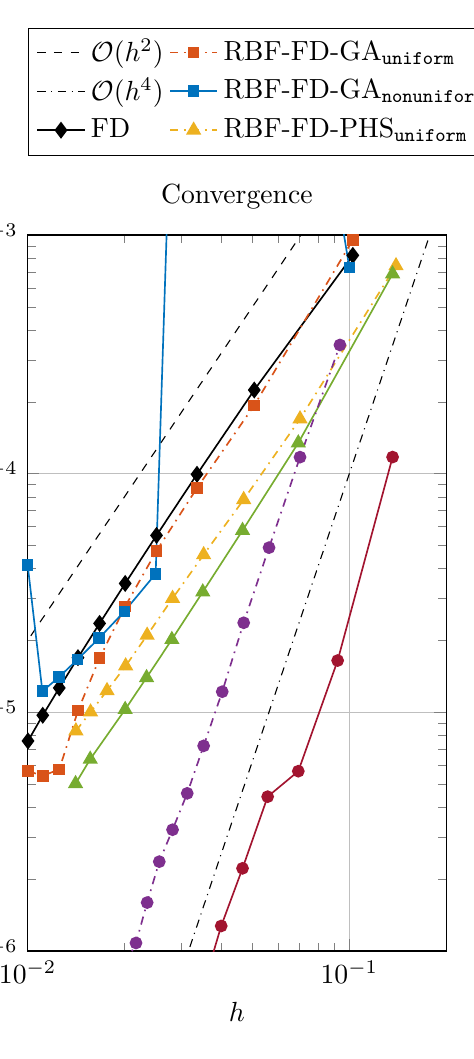
\begin{tikzpicture}[trim axis left, trim axis right, baseline]
  \begin{axis}[
  grid=major,
  width=0.4383\textwidth,
  height=0.75\textwidth,
  at={(0\textwidth,0\textwidth)},
  scale only axis,
  unbounded coords=jump,
  % x axis
  xmode=log, %this triggers the log scale
  xmin=1e-02,
  xmax=2e-01,
  xlabel={$h$},
  xminorticks=true,
  % y axis
  ymode=log,
  ymin=1e-06,
  ymax=1e-03,
  yminorticks=true,
  ytick distance=10^1, %this sets the tick distance
  ylabel={$\Delta u_{\max}$},
  %title style={font=\bfseries}, % uncomment for bold title
  title={Convergence},
  legend columns=3,
  transpose legend,
  legend style={legend cell align=left, align=left, at={(0,1.2)}, anchor=west}
  ]

  \addplot [color=black, thin, dashed]
    table[row sep=crcr, y expr=\thisrow{Y}*2]{%
    X Y\\
  0.001	1e-07\\
  0.00125892541179417	1.58489319246111e-07\\
  0.00158489319246111	2.51188643150958e-07\\
  0.00199526231496888	3.98107170553497e-07\\
  0.00251188643150958	6.30957344480193e-07\\
  0.00316227766016838	1e-06\\
  0.00398107170553497	1.58489319246111e-06\\
  0.00501187233627272	2.51188643150958e-06\\
  0.00630957344480193	3.98107170553497e-06\\
  0.00794328234724281	6.30957344480193e-06\\
  0.01	1e-05\\
  0.0125892541179417	1.58489319246111e-05\\
  0.0158489319246111	2.51188643150958e-05\\
  0.0199526231496888	3.98107170553497e-05\\
  0.0251188643150958	6.30957344480194e-05\\
  0.0316227766016838	0.0001\\
  0.0398107170553497	0.000158489319246111\\
  0.0501187233627272	0.000251188643150958\\
  0.0630957344480193	0.000398107170553497\\
  0.0794328234724281	0.000630957344480193\\
  0.1	0.001\\
  0.125892541179417	0.00158489319246111\\
  0.158489319246111	0.00251188643150958\\
  0.199526231496888	0.00398107170553497\\
  0.251188643150958	0.00630957344480193\\
  0.316227766016838	0.01\\
  0.398107170553497	0.0158489319246111\\
  0.501187233627272	0.0251188643150958\\
  0.630957344480193	0.0398107170553497\\
  0.794328234724281	0.0630957344480193\\
  1	0.1\\
  };
  \addlegendentry{$\mathcal{O}(h^2)$}

  \addplot [color=black, thin, dashdotted]
    table[row sep=crcr]{%
  0.001	1e-12\\
  0.00125892541179417	2.51188643150958e-12\\
  0.00158489319246111	6.30957344480194e-12\\
  0.00199526231496888	1.58489319246111e-11\\
  0.00251188643150958	3.98107170553497e-11\\
  0.00316227766016838	1e-10\\
  0.00398107170553497	2.51188643150958e-10\\
  0.00501187233627272	6.30957344480194e-10\\
  0.00630957344480193	1.58489319246111e-09\\
  0.00794328234724281	3.98107170553497e-09\\
  0.01	1e-08\\
  0.0125892541179417	2.51188643150958e-08\\
  0.0158489319246111	6.30957344480194e-08\\
  0.0199526231496888	1.58489319246111e-07\\
  0.0251188643150958	3.98107170553498e-07\\
  0.0316227766016838	1e-06\\
  0.0398107170553497	2.51188643150958e-06\\
  0.0501187233627272	6.30957344480193e-06\\
  0.0630957344480193	1.58489319246111e-05\\
  0.0794328234724281	3.98107170553497e-05\\
  0.1	0.0001\\
  0.125892541179417	0.000251188643150958\\
  0.158489319246111	0.000630957344480193\\
  0.199526231496888	0.00158489319246111\\
  0.251188643150958	0.00398107170553497\\
  0.316227766016838	0.01\\
  0.398107170553497	0.0251188643150958\\
  0.501187233627272	0.0630957344480193\\
  0.630957344480193	0.158489319246111\\
  0.794328234724281	0.398107170553497\\
  1	1\\
  };
  \addlegendentry{$\mathcal{O}(h^4)$}

  \addplot [color=black, semithick, mark=diamond*, mark options={scale = 1.3, solid, black}]
    table[row sep=crcr]{%
    0.0100250626566416	7.5886574535161e-06\\
    0.011142061281337	9.72228147643741e-06\\
    0.0125391849529781	1.26596809826227e-05\\
    0.014336917562724	1.69486755397803e-05\\
    0.0167364016736402	2.35866771239822e-05\\
    0.0201005025125628	3.46796687033725e-05\\
    0.0251572327044025	5.51237913711251e-05\\
    0.0336134453781513	9.94080377643199e-05\\
    0.0506329113924051	0.000224138718419901\\
    0.102564102564103	0.000821697635051559\\
  };
  \addlegendentry{$\text{FD}$}

  \addplot [color=ultikzred, semithick, dashdotted, mark=square*, mark options={scale = 0.9,solid, ultikzred}]
    table[row sep=crcr]{%
    0.0100250626566416	5.67489189767789e-06\\
  0.011142061281337	5.4245897675026e-06\\
  0.0125391849529781	5.76537132542312e-06\\
  0.014336917562724	1.01673887758155e-05\\
  0.0167364016736402	1.68818812815268e-05\\
  0.0201005025125628	2.78000505424987e-05\\
  0.0251572327044025	4.74942057093787e-05\\
  0.0336134453781513	8.70798482893939e-05\\
  0.0506329113924051	0.000193301090642285\\
  0.102564102564103	0.000954288395106928\\
  };
  \addlegendentry{$\text{RBF-FD-GA}_{\texttt{uniform}}$}

  \addplot [color=ultikzblue, semithick, mark=square*, mark options={scale = 0.9, solid, ultikzblue}]
    table[row sep=crcr]{%
    0.01	4.14165843865555e-05\\
  0.0111111111111111	1.22566457229217e-05\\
  0.0125	1.40298458809716e-05\\
  0.0142857142857143	1.664986889751e-05\\
  0.0166666666666667	2.04396388880333e-05\\
  0.02	2.64971538777616e-05\\
  0.025	3.80636671498055e-05\\
  0.0333333333333333	6.40359806
  0.05	0.000153151719320656\\
  0.1	0.000730421951017157\\
  };
  \addlegendentry{$\text{RBF-FD-GA}_{\texttt{nonuniform}}$}

  \addplot [color=ultikzyellow, semithick, dashdotted, mark=triangle*, mark options={scale = 1.3,solid, ultikzyellow}]
    table[row sep=crcr]{%
    0.014124491030929	8.36410001815724e-06\\
  0.0156917051052617	1.0028502564801e-05\\
  0.0176501127404552	1.23307428878117e-05\\
  0.0201670703622372	1.56518944708431e-05\\
  0.0235212743230775	2.10393559688313e-05\\
  0.0282138246343439	3.00189176842408e-05\\
  0.0352453688425121	4.57511141431395e-05\\
  0.046945252681302	7.78916616573505e-05\\
  0.0702728368926307	0.000169616596950958\\
  0.139686059153916	0.000743167977149496\\
  };
  \addlegendentry{$\text{RBF-FD-PHS}_{\texttt{uniform}}$}

  \addplot [color=ultikzgreen, semithick, mark=triangle*, mark options={scale = 1.3,solid, ultikzgreen}]
    table[row sep=crcr]{%
    0.0140893116711202	5.02720013236327e-06\\
  0.0156482978157298	6.36362730365575e-06
  0.0175952133454409	7.93251233059677e-06\\
  0.0200954286780432	1.02810154664346e-05\\
  0.0234238773236666	1.39793874041304e-05\\
  0.028073804789235	2.01883525170823e-05\\
  0.0350271291661823	3.19452679388398e-05\\
  0.046558865430144	5.78232547853892e-05\\
  0.0694105608393805	0.000134546330187221\\
  0.136319635318199	0.000687264699283568\\
  };
  \addlegendentry{$\text{RBF-FD-PHS}_{\texttt{nonuniform}}$}

  \addplot [color=ultikzpurple, semithick, dashdotted, mark=*, mark options={solid, ultikzpurple}]
    table[row sep=crcr]{%
  0.0201670703622372	8.86676792243582e-07\\
  0.0217154113994819	1.08094053489867e-06\\
  0.0235212743230775	1.59605544365503e-06\\
  0.0256547337551516	2.36856397064627e-06\\
  0.0282138246343439	3.22326044284102e-06\\
  0.0313400329814846	4.57864276742076e-06\\
  0.0352453688425121	7.23881122826828e-06\\
  0.0402625627785849	1.22034416352584e-05\\
  0.046945252681302	2.37328354763949e-05\\
  0.0562878035784234	4.89880039680132e-05\\
  0.0702728368926307	0.000117282713859648\\
  0.0935049164424369	0.000346118628974414\\
  };
  \addlegendentry{$\text{RBF-FD-PHS}^{\texttt{smoothed}}_{\texttt{uniform}}$}

  \addplot [color=ultikzburgundy, semithick, mark=*, mark options={solid, ultikzburgundy}]
    table[row sep=crcr]{%
    0.0350271291661823	6.99972089132939e-07\\
    0.0399780181333785	1.27354519761577e-06\\
    0.046558865430144	2.22068321180727e-06\\
    0.0557332304127295	4.43330995397034e-06\\
    0.0694105608393805	5.66874455900854e-06\\
    0.0919844099636548	1.64849648476599e-05\\
    0.136319635318199	0.000117373463206207\\
  };
  \addlegendentry{$\text{RBF-FD-PHS}^{\texttt{smoothed}}_{\texttt{nonuniform}}$}
\end{axis}
\end{tikzpicture}%

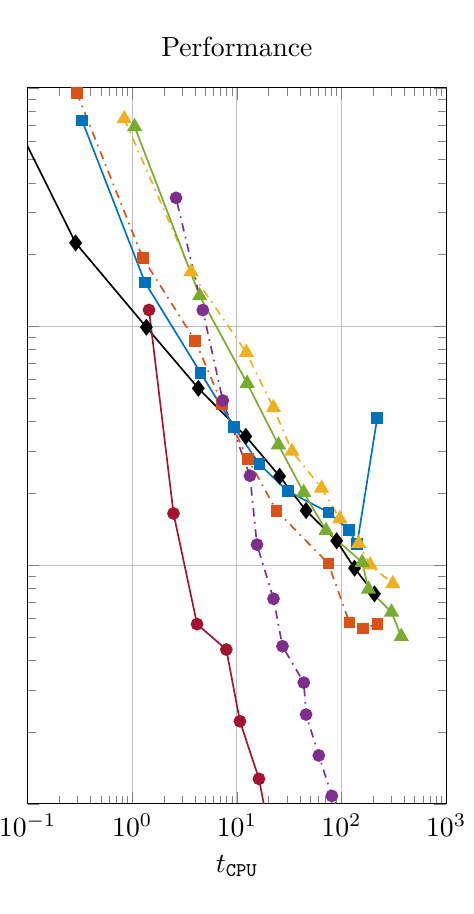
\begin{tikzpicture}[trim axis left, trim axis right, baseline]
  \begin{axis}[
  grid=major,
  width=0.4383\textwidth,
  height=0.75\textwidth,
  at={(0\textwidth,0\textwidth)},
  scale only axis,
  unbounded coords=jump,%
%x axis
  xmode=log,
  xmin=1e-01,
  xmax=1000,
  xlabel={$t_\texttt{CPU}$},%
%y axis
  ymode=log,
  ymin=1e-06,
  ymax=1e-03,
  yticklabels={,,}, %hides y ticks
  yminorticks=true,
  ytick distance=10^1,
  xminorticks=true,
  xmajorgrids,
  % xminorgrids,
  ymajorgrids,
  % yminorgrids,
  %ylabel={$\Delta u$},
  axis background/.style={fill=white},
  %title style={font=\bfseries},
  title={{\color{white}g} Performance {\color{white}g}},
  legend pos=north east,
  legend style={legend cell align=left,align=left}
  ]
  \addplot [color=black, semithick, mark=diamond*, mark options={scale = 1.3, solid, black}]
    table[row sep=crcr]{%
    0.06582786	0.000821697635051559\\
    0.287278344	0.000224138718419901\\
    1.363033105	9.94080377643199e-05\\
    4.280939024	5.51237913711251e-05\\
    12.175330572	3.46796687033725e-05\\
    25.616239575	2.35866771239822e-05\\
    45.866742939	1.69486755397803e-05\\
    89.876309784	1.26596809826227e-05\\
    133.115589004	9.72228147643741e-06\\
    206.569398646	7.5886574535161e-06\\
  };
  \addlegendentry{fd2}

  \addplot [color=ultikzred, semithick, dashdotted, mark=square*, mark options={scale = 0.9, solid, ultikzred}]
    table[row sep=crcr]{%
    0.294333181	0.000954288395106928\\
    1.264234185	0.000193301090642285\\
    4.002661134	8.70798482893939e-05\\
    7.21062104	4.74942057093787e-05\\
    12.789741194	2.78000505424987e-05\\
    23.987790138	1.68818812815268e-05\\
    74.876368296	1.01673887758155e-05\\
    118.737986566	5.76537132542312e-06\\
    160.362616102	5.4245897675026e-06\\
    220.215181191	5.67489189767789e-06\\
  };
  \addlegendentry{gs reg}

  \addplot [color=ultikzblue, semithick, mark=square*, mark options={scale = 0.9, solid, ultikzblue}]
    table[row sep=crcr]{%
    0.331154439	0.000730421951017157\\
    1.321707978	0.000153151719320656\\
    4.492199157	6.40359806401113e-05\\
    9.359380277	3.80636671498055e-05\\
    16.399435412	2.64971538777616e-05\\
    30.67468922	2.04396388880333e-05\\
    75.199079076	1.664986889751e-05\\
    117.664701023	1.40298458809716e-05\\
    140.823239139	1.22566457229217e-05\\
    219.44733059	4.14165843865555e-05\\
  };
  \addlegendentry{gs adap}

  \addplot [color=ultikzyellow, semithick, dashdotted, mark=triangle*, mark options={scale = 1.3,solid, ultikzyellow}]
    table[row sep=crcr]{%
    0.837605647	0.000743167977149496\\
  3.639769825	0.000169616596950958\\
  12.290603411	7.78916616573505e-05\\
  22.358980677	4.57511141431395e-05\\
  33.609578206	3.00189176842408e-05\\
  64.471801581	2.10393559688313e-05\\
  96.176644434	1.56518944708431e-05\\
  145.624530492	1.23307428878117e-05\\
  187.614598032	1.0028502564801e-05\\
  309.252198757	8.36410001815724e-06\\
  };
  \addlegendentry{phs reg}

  \addplot [color=ultikzgreen, semithick, mark=triangle*, mark options={scale = 1.3,solid, ultikzgreen}]
    table[row sep=crcr]{%
    1.053425471	0.000687264699283568\\
    4.408053073	0.000134546330187221\\
    12.539242522	5.78232547853892e-05\\
    24.935753374	3.19452679388398e-05\\
    43.468228217	2.01883525170823e-05\\
    71.169584803	1.39793874041304e-05\\
    157.613770699	1.02810154664346e-05\\
    181.066750603	7.93251233059677e-06\\
    300.717458059	6.36362730365575e-06\\
    372.861778238	5.02720013236327e-06\\
  };
  \addlegendentry{phs adap}

  \addplot [color=ultikzpurple, semithick, dashdotted, mark=*, mark options={solid, ultikzpurple}]
    table[row sep=crcr]{%
    100.308480392	8.86676792243582e-07\\
    80.801123362	1.08094053489867e-06\\
    60.677620782	1.59605544365503e-06\\
    45.861328437	2.36856397064627e-06\\
    43.590460923	3.22326044284102e-06\\
    27.272527995	4.57864276742076e-06\\
    22.378082203	7.23881122826828e-06\\
    15.556166938	1.22034416352584e-05\\
    13.325419311	2.37328354763949e-05\\
    7.335637489	4.89880039680132e-05\\
    4.719910087	0.000117282713859648\\
    2.619557301	0.000346118628974414\\
  };
  \addlegendentry{phs reg smoothed}

  \addplot [color=ultikzburgundy, semithick, mark=*, mark options={solid, ultikzburgundy}]
    table[row sep=crcr]{%
    1.444674318	0.000117373463206207\\
    2.478047665	1.64849648476599e-05\\
    4.160072468	5.66874455900854e-06\\
    7.925728684	4.43330995397034e-06\\
    10.689505454	2.22068321180727e-06\\
    16.261363834	1.27354519761577e-06\\
    21.123572908	6.99972089132939e-07\\
  };
  \addlegendentry{phs adap smoothed}
  \legend{};
\end{axis}
\end{tikzpicture}%

\caption{\emph{Convergence and computational performance.}}
\label{fig:log}
\end{figure}
%
\subsection{Custom Ticks}
%
\begin{figure}[H]
\centering
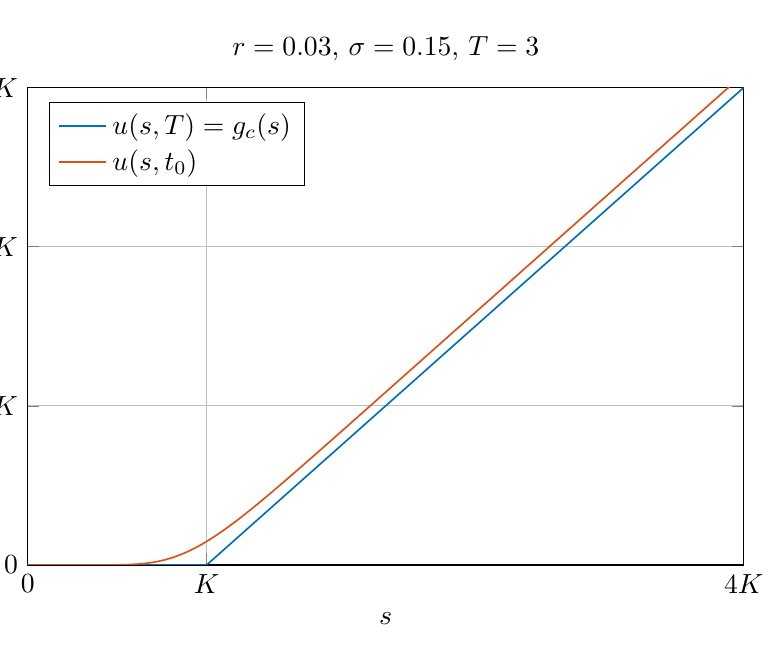
\begin{tikzpicture}[trim axis left, trim axis right, baseline]
\begin{axis}[%
% dimensions
width=0.75\textwidth,
height=0.5\textwidth,
at={(0\textwidth,0\textwidth)},
scale only axis, %
% limits
xmin=0,
xmax=400,
ymin=0,
ymax=300,%
% gridlines
xmajorgrids,
ymajorgrids,%
% ticks
xtick={0,100,400},
xticklabels={$0$,$K$,$4K$},
ytick={0,100,200,300,400},
yticklabels={$0$,$K$,$2K$,$3K$,$4K$},%
% labels
xlabel={$s$},
ylabel={$u(s,t)$},
title={$r=0.03$, $\sigma=0.15$, $T=3$},
% legend
legend style={legend cell align=left, align=left},
legend pos = north west,
]
\addplot [color=ultikzblue, semithick] %the first line, other lines are added just like this
  table[row sep=crcr]{% paste data here
0	0\\
4.04040404040404	0\\
8.08080808080808	0\\
12.1212121212121	0\\
16.1616161616162	0\\
20.2020202020202	0\\
24.2424242424242	0\\
28.2828282828283	0\\
32.3232323232323	0\\
36.3636363636364	0\\
40.4040404040404	0\\
44.4444444444444	0\\
48.4848484848485	0\\
52.5252525252525	0\\
56.5656565656566	0\\
60.6060606060606	0\\
64.6464646464647	0\\
68.6868686868687	0\\
72.7272727272727	0\\
76.7676767676768	0\\
80.8080808080808	0\\
84.8484848484848	0\\
88.8888888888889	0\\
92.9292929292929	0\\
96.969696969697	0\\
100 0\\
101.010101010101	1.01010101010101\\
105.050505050505	5.05050505050505\\
109.090909090909	9.09090909090909\\
113.131313131313	13.1313131313131\\
117.171717171717	17.1717171717172\\
121.212121212121	21.2121212121212\\
125.252525252525	25.2525252525252\\
129.292929292929	29.2929292929293\\
133.333333333333	33.3333333333333\\
137.373737373737	37.3737373737374\\
141.414141414141	41.4141414141414\\
145.454545454545	45.4545454545455\\
149.49494949495	49.4949494949495\\
153.535353535354	53.5353535353535\\
157.575757575758	57.5757575757576\\
161.616161616162	61.6161616161616\\
165.656565656566	65.6565656565656\\
169.69696969697	69.6969696969697\\
173.737373737374	73.7373737373737\\
177.777777777778	77.7777777777778\\
181.818181818182	81.8181818181818\\
185.858585858586	85.8585858585859\\
189.89898989899	89.8989898989899\\
193.939393939394	93.9393939393939\\
197.979797979798	97.979797979798\\
202.020202020202	102.020202020202\\
206.060606060606	106.060606060606\\
210.10101010101	110.10101010101\\
214.141414141414	114.141414141414\\
218.181818181818	118.181818181818\\
222.222222222222	122.222222222222\\
226.262626262626	126.262626262626\\
230.30303030303	130.30303030303\\
234.343434343434	134.343434343434\\
238.383838383838	138.383838383838\\
242.424242424242	142.424242424242\\
246.464646464646	146.464646464646\\
250.50505050505	150.50505050505\\
254.545454545455	154.545454545455\\
258.585858585859	158.585858585859\\
262.626262626263	162.626262626263\\
266.666666666667	166.666666666667\\
270.707070707071	170.707070707071\\
274.747474747475	174.747474747475\\
278.787878787879	178.787878787879\\
282.828282828283	182.828282828283\\
286.868686868687	186.868686868687\\
290.909090909091	190.909090909091\\
294.949494949495	194.949494949495\\
298.989898989899	198.989898989899\\
303.030303030303	203.030303030303\\
307.070707070707	207.070707070707\\
311.111111111111	211.111111111111\\
315.151515151515	215.151515151515\\
319.191919191919	219.191919191919\\
323.232323232323	223.232323232323\\
327.272727272727	227.272727272727\\
331.313131313131	231.313131313131\\
335.353535353535	235.353535353535\\
339.393939393939	239.393939393939\\
343.434343434343	243.434343434343\\
347.474747474747	247.474747474747\\
351.515151515152	251.515151515152\\
355.555555555556	255.555555555556\\
359.59595959596	259.59595959596\\
363.636363636364	263.636363636364\\
367.676767676768	267.676767676768\\
371.717171717172	271.717171717172\\
375.757575757576	275.757575757576\\
379.79797979798	279.79797979798\\
383.838383838384	283.838383838384\\
387.878787878788	287.878787878788\\
391.919191919192	291.919191919192\\
395.959595959596	295.959595959596\\
400	300\\
};
\addlegendentry{$u(s,T)=g_c(s)$}

\addplot [color=ultikzred, semithick]
  table[row sep=crcr]{%
0	0\\
4.04040404040404	0\\
8.08080808080808	0\\
12.1212121212121	4.06518274685513e-15\\
16.1616161616162	1.84110226260438e-11\\
20.2020202020202	5.6570893425188e-09\\
24.2424242424242	3.61754452061055e-07\\
28.2828282828283	8.47218861555263e-06\\
32.3232323232323	9.98647852595565e-05\\
36.3636363636364	0.00071966703651701\\
40.4040404040404	0.00359845105956065\\
44.4444444444444	0.0136101617332664\\
48.4848484848485	0.0413941343712883\\
52.5252525252525	0.105862922529326\\
56.5656565656566	0.235403119330865\\
60.6060606060606	0.466944235830593\\
64.6464646464647	0.842883472743563\\
68.6868686868687	1.40662006030599\\
72.7272727272727	2.19781847486442\\
76.7676767676768	3.2484302386748\\
80.8080808080808	4.58012154573924\\
84.8484848484848	6.203297849965\\
88.8888888888889	8.1175485478212\\
92.9292929292929	10.3131237730385\\
96.969696969697	12.7729952067817\\
101.010101010101	15.4750993178966\\
105.050505050505	18.3944625991648\\
109.090909090909	21.5050221822407\\
113.131313131313	24.7810555196482\\
117.171717171717	28.1982078353119\\
121.212121212121	31.7341540722855\\
125.252525252525	35.3689570104479\\
129.292929292929	39.0851911389302\\
133.333333333333	42.8678988009122\\
137.373737373737	46.7044360787997\\
141.414141414141	50.58425447158\\
145.454545454545	54.498652955167\\
149.49494949495	58.440524802846\\
153.535353535354	62.4041151394003\\
157.575757575758	66.3847987080162\\
161.616161616162	70.3788825821819\\
165.656565656566	74.3834352748955\\
169.69696969697	78.3961415734878\\
173.737373737374	82.4151811686068\\
177.777777777778	86.4391285016292\\
181.818181818182	90.4668710271427\\
185.858585858586	94.4975431252303\\
189.89898989899	98.5304730924492\\
193.939393939394	102.565140914428\\
197.979797979798	106.601144826313\\
202.020202020202	110.638174968188\\
206.060606060606	114.67599272272\\
210.10101010101	118.714414572371\\
214.141414141414	122.753299530226\\
218.181818181818	126.792539382121\\
222.222222222222	130.832051130643\\
226.262626262626	134.871771157106\\
230.30303030303	138.911650719532\\
234.343434343434	142.951652486606\\
238.383838383838	146.991747872971\\
242.424242424242	151.031914993026\\
246.464646464646	155.072137091239\\
250.50505050505	159.112401339001\\
254.545454545455	163.152697913036\\
258.585858585859	167.193019289856\\
262.626262626263	171.233359705835\\
266.666666666667	175.273714744121\\
270.707070707071	179.314081018674\\
274.747474747475	183.354455932582\\
278.787878787879	187.394837493224\\
282.828282828283	191.435224170864\\
286.868686868687	195.475614790484\\
290.909090909091	199.516008449002\\
294.949494949495	203.556404451913\\
298.989898989899	207.596802264768\\
303.030303030303	211.637201476017\\
307.070707070707	215.677601768527\\
311.111111111111	219.718002897743\\
315.151515151515	223.758404674944\\
319.191919191919	227.798806954384\\
323.232323232323	231.839209623421\\
327.272727272727	235.879612594926\\
331.313131313131	239.920015801456\\
335.353535353535	243.960419190761\\
339.393939393939	248.000822722328\\
343.434343434343	252.04122636472\\
347.474747474747	256.081630093523\\
351.515151515152	260.122033889758\\
355.555555555556	264.162437738662\\
359.59595959596	268.202841628739\\
363.636363636364	272.243245551032\\
367.676767676768	276.283649498554\\
371.717171717172	280.324053465851\\
375.757575757576	284.36445744866\\
379.79797979798	288.404861443651\\
383.838383838384	292.445265448215\\
387.878787878788	296.485669460309\\
391.919191919192	300.526073478331\\
395.959595959596	304.566477501024\\
400	308.606881527401\\
};
\addlegendentry{$u(s,t_0)$}

\end{axis}
\end{tikzpicture}%

\caption{\emph{Examples of GAs with different shape parameter values and PHSs of different degrees.}}
\label{fig:payoff}
\end{figure}
%
%
%
\newpage
\section{Scatter Plots}
Here is an example of a scatter plot.
\begin{figure}[H]
\centering
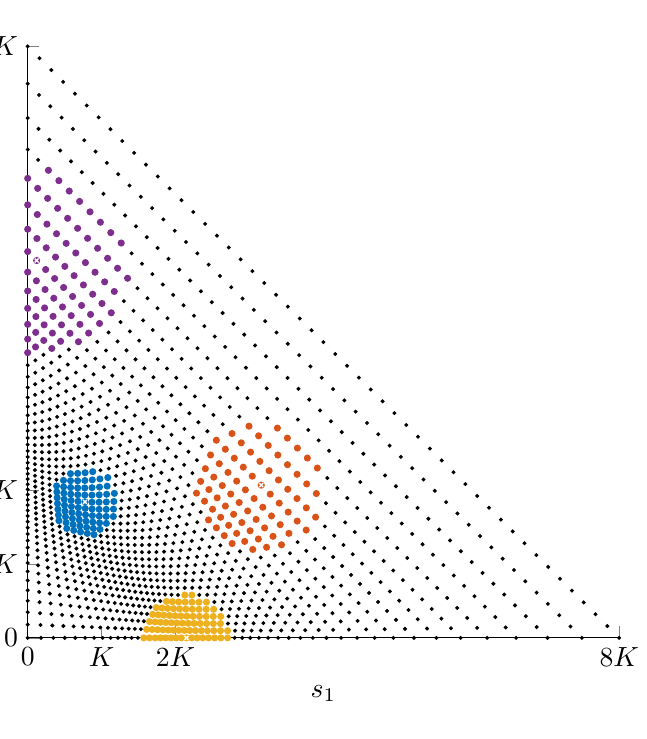
\begin{tikzpicture}[trim axis left, trim axis right]
\begin{axis}[%
axis x line*=bottom, %removes the box
axis y line*=left, %removes the box
% dimension
width=0.75\textwidth,
height=0.75\textwidth,
xmin=0,
xmax=8,
ymin=0,
ymax=8,
% tick and labels
xtick={0,1,2,8},
xticklabels={$0$,$K$,$2K$,$8K$},
% xticklabels={}, %uncomment to remove all xticklabels
ytick={0,1,2,8},
yticklabels={$0$,$K$,$2K$,$8K$},
% yticklabels={}, %uncomment to remove all yticklabels
xlabel={$s_1$},
ylabel={$s_2$},
]
\addplot [color=black, mark size=0.5pt, only marks, mark=*, mark options={solid}, forget plot]
  table[row sep=crcr]{%
  0	0\\
  0	0.180451956615514\\
  0.180451956615514	0\\
  0	0.347061520741313\\
  0.173530760370657	0.173530760370657\\
  0.347061520741313	0\\
  0	0.501096191187092\\
  0.167032063729031	0.334064127458061\\
  0.334064127458061	0.167032063729031\\
  0.501096191187092	0\\
  0	0.643727802009712\\
  0.160931950502428	0.482795851507284\\
  0.321863901004856	0.321863901004856\\
  0.482795851507284	0.160931950502428\\
  0.643727802009712	0\\
  0	0.776041437357198\\
  0.15520828747144	0.620833149885759\\
  0.310416574942879	0.465624862414319\\
  0.465624862414319	0.310416574942879\\
  0.620833149885759	0.15520828747144\\
  0.776041437357198	0\\
  0	0.899043686354185\\
  0.149840614392364	0.749203071961821\\
  0.299681228784728	0.599362457569457\\
  0.449521843177093	0.449521843177093\\
  0.599362457569457	0.299681228784728\\
  0.749203071961821	0.149840614392364\\
  0.899043686354185	0\\
  0	1.01367030082868\\
  0.144810042975525	0.86886025785315\\
  0.28962008595105	0.724050214877625\\
  0.434430128926575	0.5792401719021\\
  0.5792401719021	0.434430128926575\\
  0.724050214877625	0.28962008595105\\
  0.86886025785315	0.144810042975525\\
  1.01367030082868	0\\
  0	1.12079331413702\\
  0.140099164267128	0.980694149869895\\
  0.280198328534256	0.840594985602767\\
  0.420297492801383	0.700495821335639\\
  0.560396657068511	0.560396657068511\\
  0.700495821335639	0.420297492801383\\
  0.840594985602767	0.280198328534256\\
  0.980694149869895	0.140099164267128\\
  1.12079331413702	0\\
  0	1.22122767524432\\
  0.135691963916036	1.08553571132829\\
  0.271383927832072	0.949843747412251\\
  0.407075891748107	0.814151783496215\\
  0.542767855664143	0.678459819580179\\
  0.678459819580179	0.542767855664143\\
  0.814151783496215	0.407075891748107\\
  0.949843747412251	0.271383927832072\\
  1.08553571132829	0.135691963916036\\
  1.22122767524432	0\\
  0	1.31573744852961\\
  0.131573744852961	1.18416370367665\\
  0.263147489705923	1.05258995882369\\
  0.394721234558884	0.921016213970729\\
  0.526294979411845	0.789442469117768\\
  0.657868724264807	0.657868724264807\\
  0.789442469117768	0.526294979411845\\
  0.921016213970729	0.394721234558884\\
  1.05258995882369	0.263147489705923\\
  1.18416370367665	0.131573744852961\\
  1.31573744852961	0\\
  0	1.40504162648154\\
  0.127731056952868	1.27731056952868\\
  0.255462113905735	1.14957951257581\\
  0.383193170858603	1.02184845562294\\
  0.510924227811471	0.894117398670074\\
  0.638655284764338	0.766386341717206\\
  0.766386341717206	0.638655284764338\\
  0.894117398670074	0.510924227811471\\
  1.02184845562294	0.383193170858603\\
  1.14957951257581	0.255462113905735\\
  1.27731056952868	0.127731056952868\\
  1.40504162648154	0\\
  0	1.48981959950515\\
  0.124151633292096	1.36566796621306\\
  0.248303266584192	1.24151633292096\\
  0.372454899876289	1.11736469962887\\
  0.496606533168385	0.99321306633677\\
  0.620758166460481	0.869061433044674\\
  0.744909799752577	0.744909799752577\\
  0.869061433044674	0.620758166460481\\
  0.99321306633677	0.496606533168385\\
  1.11736469962887	0.372454899876289\\
  1.24151633292096	0.248303266584192\\
  1.36566796621306	0.124151633292096\\
  1.48981959950515	0\\
  0	1.57071632445187\\
  0.120824332650144	1.44989199180172\\
  0.241648665300287	1.32906765915158\\
  0.362472997950431	1.20824332650144\\
  0.483297330600574	1.08741899385129\\
  0.604121663250718	0.966594661201149\\
  0.724945995900862	0.845770328551005\\
  0.845770328551005	0.724945995900862\\
  0.966594661201149	0.604121663250718\\
  1.08741899385129	0.483297330600574\\
  1.20824332650144	0.362472997950431\\
  1.32906765915158	0.241648665300287\\
  1.44989199180172	0.120824332650144\\
  1.57071632445187	0\\
  0	1.64834723119281\\
  0.117739087942343	1.53060814325046\\
  0.235478175884687	1.41286905530812\\
  0.35321726382703	1.29512996736578\\
  0.470956351769373	1.17739087942343\\
  0.588695439711716	1.05965179148109\\
  0.70643452765406	0.941912703538746\\
  0.824173615596403	0.824173615596403\\
  0.941912703538746	0.70643452765406\\
  1.05965179148109	0.588695439711716\\
  1.17739087942343	0.470956351769373\\
  1.29512996736578	0.35321726382703\\
  1.41286905530812	0.235478175884687\\
  1.53060814325046	0.117739087942343\\
  1.64834723119281	0\\
  0	1.72330290456268\\
  0.114886860304178	1.6084160442585\\
  0.229773720608357	1.49352918395432\\
  0.344660580912535	1.37864232365014\\
  0.459547441216714	1.26375546334596\\
  0.574434301520892	1.14886860304178\\
  0.689321161825071	1.03398174273761\\
  0.804208022129249	0.919094882433428\\
  0.919094882433428	0.804208022129249\\
  1.03398174273761	0.689321161825071\\
  1.14886860304178	0.574434301520892\\
  1.26375546334596	0.459547441216714\\
  1.37864232365014	0.344660580912535\\
  1.49352918395432	0.229773720608357\\
  1.6084160442585	0.114886860304178\\
  1.72330290456268	0\\
  0	1.79615357729256\\
  0.112259598580785	1.68389397871178\\
  0.22451919716157	1.57163438013099\\
  0.336778795742356	1.45937478155021\\
  0.449038394323141	1.34711518296942\\
  0.561297992903926	1.23485558438864\\
  0.673557591484711	1.12259598580785\\
  0.785817190065496	1.01033638722707\\
  0.898076788646281	0.898076788646281\\
  1.01033638722707	0.785817190065496\\
  1.12259598580785	0.673557591484711\\
  1.23485558438864	0.561297992903926\\
  1.34711518296942	0.449038394323141\\
  1.45937478155021	0.336778795742356\\
  1.57163438013099	0.22451919716157\\
  1.68389397871178	0.112259598580785\\
  1.79615357729256	0\\
  0	1.86745346811207\\
  0.109850204006593	1.75760326410548\\
  0.219700408013185	1.64775306009889\\
  0.329550612019778	1.5379028560923\\
  0.43940081602637	1.4280526520857\\
  0.549251020032963	1.31820244807911\\
  0.659101224039555	1.20835224407252\\
  0.768951428046148	1.09850204006593\\
  0.87880163205274	0.988651836059333\\
  0.988651836059333	0.87880163205274\\
  1.09850204006593	0.768951428046148\\
  1.20835224407252	0.659101224039555\\
  1.31820244807911	0.549251020032963\\
  1.4280526520857	0.43940081602637\\
  1.5379028560923	0.329550612019778\\
  1.64775306009889	0.219700408013185\\
  1.75760326410548	0.109850204006593\\
  1.86745346811207	0\\
  0	1.93774499802338\\
  0.107652499890188	1.83009249813319\\
  0.215304999780376	1.72243999824301\\
  0.322957499670564	1.61478749835282\\
  0.430609999560752	1.50713499846263\\
  0.538262499450939	1.39948249857244\\
  0.645914999341127	1.29182999868225\\
  0.753567499231315	1.18417749879207\\
  0.861219999121503	1.07652499890188\\
  0.968872499011691	0.968872499011691\\
  1.07652499890188	0.861219999121503\\
  1.18417749879207	0.753567499231315\\
  1.29182999868225	0.645914999341127\\
  1.39948249857244	0.53826249945094\\
  1.50713499846263	0.430609999560752\\
  1.61478749835282	0.322957499670564\\
  1.72243999824301	0.215304999780376\\
  1.83009249813319	0.107652499890188\\
  1.93774499802338	0\\
  0	2.00756291682289\\
  0.105661206148573	1.90190171067431\\
  0.211322412297146	1.79624050452574\\
  0.316983618445719	1.69057929837717\\
  0.422644824594292	1.5849180922286\\
  0.528306030742865	1.47925688608002\\
  0.633967236891438	1.37359567993145\\
  0.739628443040011	1.26793447378288\\
  0.845289649188584	1.1622732676343\\
  0.950950855337157	1.05661206148573\\
  1.05661206148573	0.950950855337157\\
  1.1622732676343	0.845289649188584\\
  1.26793447378288	0.739628443040011\\
  1.37359567993145	0.633967236891438\\
  1.47925688608002	0.528306030742865\\
  1.5849180922286	0.422644824594292\\
  1.69057929837717	0.316983618445719\\
  1.79624050452574	0.211322412297146\\
  1.90190171067431	0.105661206148573\\
  2.00756291682289	0\\
  0	2.0774383712634\\
  0.10387191856317	1.97356645270023\\
  0.20774383712634	1.86969453413706\\
  0.311615755689511	1.76582261557389\\
  0.415487674252681	1.66195069701072\\
  0.519359592815851	1.55807877844755\\
  0.623231511379021	1.45420685988438\\
  0.727103429942191	1.35033494132121\\
  0.830975348505362	1.24646302275804\\
  0.934847267068532	1.14259110419487\\
  1.0387191856317	1.0387191856317\\
  1.14259110419487	0.934847267068532\\
  1.24646302275804	0.830975348505362\\
  1.35033494132121	0.727103429942192\\
  1.45420685988438	0.623231511379021\\
  1.55807877844755	0.519359592815851\\
  1.66195069701072	0.415487674252681\\
  1.76582261557389	0.311615755689511\\
  1.86969453413706	0.20774383712634\\
  1.97356645270023	0.10387191856317\\
  2.0774383712634	0\\
  0	2.14790294580586\\
  0.102281092657422	2.04562185314843\\
  0.204562185314843	1.94334076049101\\
  0.306843277972265	1.84105966783359\\
  0.409124370629687	1.73877857517617\\
  0.511405463287108	1.63649748251875\\
  0.61368655594453	1.53421638986133\\
  0.715967648601952	1.4319352972039\\
  0.818248741259374	1.32965420454648\\
  0.920529833916795	1.22737311188906\\
  1.02281092657422	1.12509201923164\\
  1.12509201923164	1.02281092657422\\
  1.22737311188906	0.920529833916795\\
  1.32965420454648	0.818248741259374\\
  1.4319352972039	0.715967648601952\\
  1.53421638986133	0.61368655594453\\
  1.63649748251875	0.511405463287109\\
  1.73877857517617	0.409124370629687\\
  1.84105966783359	0.306843277972265\\
  1.94334076049101	0.204562185314843\\
  2.04562185314843	0.102281092657422\\
  2.14790294580586	0\\
  0	2.21949270670086\\
  0.100886032122766	2.11860667457809\\
  0.201772064245533	2.01772064245533\\
  0.302658096368299	1.91683461033256\\
  0.403544128491065	1.81594857820979\\
  0.504430160613832	1.71506254608703\\
  0.605316192736598	1.61417651396426\\
  0.706202224859364	1.5132904818415\\
  0.807088256982131	1.41240444971873\\
  0.907974289104897	1.31151841759596\\
  1.00886032122766	1.2106323854732\\
  1.10974635335043	1.10974635335043\\
  1.2106323854732	1.00886032122766\\
  1.31151841759596	0.907974289104897\\
  1.41240444971873	0.807088256982131\\
  1.51329048184149	0.706202224859364\\
  1.61417651396426	0.605316192736598\\
  1.71506254608703	0.504430160613832\\
  1.81594857820979	0.403544128491065\\
  1.91683461033256	0.302658096368299\\
  2.01772064245533	0.201772064245533\\
  2.11860667457809	0.100886032122766\\
  2.21949270670086	0\\
  0	2.29275228016598\\
  0.0996848817463471	2.19306739841964\\
  0.199369763492694	2.09338251667329\\
  0.299054645239041	1.99369763492694\\
  0.398739526985389	1.8940127531806\\
  0.498424408731736	1.79432787143425\\
  0.598109290478083	1.6946429896879\\
  0.69779417222443	1.59495810794155\\
  0.797479053970777	1.49527322619521\\
  0.897163935717124	1.39558834444886\\
  0.996848817463471	1.29590346270251\\
  1.09653369920982	1.19621858095617\\
  1.19621858095617	1.09653369920982\\
  1.29590346270251	0.996848817463472\\
  1.39558834444886	0.897163935717124\\
  1.49527322619521	0.797479053970777\\
  1.59495810794155	0.69779417222443\\
  1.6946429896879	0.598109290478083\\
  1.79432787143425	0.498424408731736\\
  1.8940127531806	0.398739526985389\\
  1.99369763492694	0.299054645239041\\
  2.09338251667329	0.199369763492694\\
  2.19306739841964	0.0996848817463469\\
  2.29275228016598	0\\
  0	2.3682389956838\\
  0.0986766248201584	2.26956237086364\\
  0.197353249640317	2.17088574604349\\
  0.296029874460475	2.07220912122333\\
  0.394706499280634	1.97353249640317\\
  0.493383124100792	1.87485587158301\\
  0.592059748920951	1.77617924676285\\
  0.690736373741109	1.67750262194269\\
  0.789412998561267	1.57882599712253\\
  0.888089623381426	1.48014937230238\\
  0.986766248201584	1.38147274748222\\
  1.08544287302174	1.28279612266206\\
  1.1841194978419	1.1841194978419\\
  1.28279612266206	1.08544287302174\\
  1.38147274748222	0.986766248201584\\
  1.48014937230238	0.888089623381426\\
  1.57882599712253	0.789412998561267\\
  1.67750262194269	0.690736373741109\\
  1.77617924676285	0.59205974892095\\
  1.87485587158301	0.493383124100792\\
  1.97353249640317	0.394706499280634\\
  2.07220912122333	0.296029874460475\\
  2.17088574604349	0.197353249640317\\
  2.26956237086364	0.0986766248201585\\
  2.3682389956838	0\\
  0	2.44652712594129\\
  0.0978610850376515	2.34866604090364\\
  0.195722170075303	2.25080495586599\\
  0.293583255112955	2.15294387082833\\
  0.391444340150606	2.05508278579068\\
  0.489305425188258	1.95722170075303\\
  0.587166510225909	1.85936061571538\\
  0.685027595263561	1.76149953067773\\
  0.782888680301212	1.66363844564008\\
  0.880749765338864	1.56577736060242\\
  0.978610850376516	1.46791627556477\\
  1.07647193541417	1.37005519052712\\
  1.17433302045182	1.27219410548947\\
  1.27219410548947	1.17433302045182\\
  1.37005519052712	1.07647193541417\\
  1.46791627556477	0.978610850376515\\
  1.56577736060242	0.880749765338864\\
  1.66363844564008	0.782888680301213\\
  1.76149953067773	0.685027595263561\\
  1.85936061571538	0.587166510225909\\
  1.95722170075303	0.489305425188258\\
  2.05508278579068	0.391444340150606\\
  2.15294387082833	0.293583255112955\\
  2.25080495586599	0.195722170075303\\
  2.34866604090364	0.0978610850376516\\
  2.44652712594129	0\\
  0	2.52821225566634\\
  0.0972389329102438	2.4309733227561\\
  0.194477865820488	2.33373438984585\\
  0.291716798730731	2.23649545693561\\
  0.388955731640975	2.13925652402536\\
  0.486194664551219	2.04201759111512\\
  0.583433597461463	1.94477865820488\\
  0.680672530371707	1.84753972529463\\
  0.77791146328195	1.75030079238439\\
  0.875150396192194	1.65306185947414\\
  0.972389329102438	1.5558229265639\\
  1.06962826201268	1.45858399365366\\
  1.16686719492293	1.36134506074341\\
  1.26410612783317	1.26410612783317\\
  1.36134506074341	1.16686719492293\\
  1.45858399365366	1.06962826201268\\
  1.5558229265639	0.972389329102438\\
  1.65306185947414	0.875150396192194\\
  1.75030079238439	0.77791146328195\\
  1.84753972529463	0.680672530371707\\
  1.94477865820488	0.583433597461463\\
  2.04201759111512	0.486194664551219\\
  2.13925652402536	0.388955731640975\\
  2.23649545693561	0.291716798730731\\
  2.33373438984585	0.194477865820488\\
  2.4309733227561	0.0972389329102441\\
  2.52821225566634	0\\
  0	2.61391581259775\\
  0.0968116967628795	2.51710411583487\\
  0.193623393525759	2.42029241907199\\
  0.290435090288639	2.32348072230911\\
  0.387246787051518	2.22666902554623\\
  0.484058483814397	2.12985732878335\\
  0.580870180577277	2.03304563202047\\
  0.677681877340157	1.93623393525759\\
  0.774493574103036	1.83942223849471\\
  0.871305270865915	1.74261054173183\\
  0.968116967628795	1.64579884496895\\
  1.06492866439167	1.54898714820607\\
  1.16174036115455	1.45217545144319\\
  1.25855205791743	1.35536375468031\\
  1.35536375468031	1.25855205791743\\
  1.45217545144319	1.16174036115455\\
  1.54898714820607	1.06492866439167\\
  1.64579884496895	0.968116967628795\\
  1.74261054173183	0.871305270865915\\
  1.83942223849471	0.774493574103036\\
  1.93623393525759	0.677681877340157\\
  2.03304563202047	0.580870180577277\\
  2.12985732878335	0.484058483814398\\
  2.22666902554623	0.387246787051518\\
  2.32348072230911	0.290435090288638\\
  2.42029241907199	0.193623393525759\\
  2.51710411583487	0.0968116967628796\\
  2.61391581259775	0\\
  0	2.70428979505846\\
  0.096581778394945	2.60770801666351\\
  0.19316355678989	2.51112623826857\\
  0.289745335184835	2.41454445987362\\
  0.38632711357978	2.31796268147868\\
  0.482908891974725	2.22138090308373\\
  0.57949067036967	2.12479912468879\\
  0.676072448764615	2.02821734629384\\
  0.77265422715956	1.9316355678989\\
  0.869236005554505	1.83505378950395\\
  0.96581778394945	1.73847201110901\\
  1.06239956234439	1.64189023271406\\
  1.15898134073934	1.54530845431912\\
  1.25556311913428	1.44872667592417\\
  1.35214489752923	1.35214489752923\\
  1.44872667592417	1.25556311913428\\
  1.54530845431912	1.15898134073934\\
  1.64189023271406	1.06239956234439\\
  1.73847201110901	0.96581778394945\\
  1.83505378950395	0.869236005554505\\
  1.9316355678989	0.77265422715956\\
  2.02821734629384	0.676072448764615\\
  2.12479912468879	0.57949067036967\\
  2.22138090308373	0.482908891974725\\
  2.31796268147868	0.38632711357978\\
  2.41454445987362	0.289745335184835\\
  2.51112623826857	0.19316355678989\\
  2.60770801666351	0.096581778394945\\
  2.70428979505846	0\\
  0	2.80002173209759\\
  0.0965524735206065	2.70346925857698\\
  0.193104947041213	2.60691678505637\\
  0.289657420561819	2.51036431153577\\
  0.386209894082426	2.41381183801516\\
  0.482762367603032	2.31725936449456\\
  0.579314841123639	2.22070689097395\\
  0.675867314644245	2.12415441745334\\
  0.772419788164852	2.02760194393274\\
  0.868972261685458	1.93104947041213\\
  0.965524735206065	1.83449699689152\\
  1.06207720872667	1.73794452337092\\
  1.15862968224728	1.64139204985031\\
  1.25518215576788	1.5448395763297\\
  1.35173462928849	1.4482871028091\\
  1.4482871028091	1.35173462928849\\
  1.5448395763297	1.25518215576788\\
  1.64139204985031	1.15862968224728\\
  1.73794452337092	1.06207720872667\\
  1.83449699689152	0.965524735206065\\
  1.93104947041213	0.868972261685458\\
  2.02760194393274	0.772419788164852\\
  2.12415441745334	0.675867314644246\\
  2.22070689097395	0.579314841123639\\
  2.31725936449456	0.482762367603032\\
  2.41381183801516	0.386209894082425\\
  2.51036431153577	0.28965742056182\\
  2.60691678505637	0.193104947041213\\
  2.70346925857698	0.0965524735206063\\
  2.80002173209759	0\\
  0	2.90183991393594\\
  0.0967279971311982	2.80511191680475\\
  0.193455994262396	2.70838391967355\\
  0.290183991393595	2.61165592254235\\
  0.386911988524793	2.51492792541115\\
  0.483639985655991	2.41819992827995\\
  0.580367982787189	2.32147193114876\\
  0.677095979918387	2.22474393401756\\
  0.773823977049585	2.12801593688636\\
  0.870551974180783	2.03128793975516\\
  0.967279971311982	1.93455994262396\\
  1.06400796844318	1.83783194549277\\
  1.16073596557438	1.74110394836157\\
  1.25746396270558	1.64437595123037\\
  1.35419195983677	1.54764795409917\\
  1.45091995696797	1.45091995696797\\
  1.54764795409917	1.35419195983677\\
  1.64437595123037	1.25746396270558\\
  1.74110394836157	1.16073596557438\\
  1.83783194549277	1.06400796844318\\
  1.93455994262396	0.967279971311982\\
  2.03128793975516	0.870551974180783\\
  2.12801593688636	0.773823977049585\\
  2.22474393401756	0.677095979918387\\
  2.32147193114876	0.580367982787189\\
  2.41819992827995	0.483639985655991\\
  2.51492792541115	0.386911988524793\\
  2.61165592254235	0.290183991393595\\
  2.70838391967355	0.193455994262396\\
  2.80511191680475	0.0967279971311981\\
  2.90183991393594	0\\
  0	3.01051893250625\\
  0.0971135139518144	2.91340541855443\\
  0.194227027903629	2.81629190460262\\
  0.291340541855443	2.7191783906508\\
  0.388454055807258	2.62206487669899\\
  0.485567569759072	2.52495136274717\\
  0.582681083710886	2.42783784879536\\
  0.679794597662701	2.33072433484355\\
  0.776908111614515	2.23361082089173\\
  0.87402162556633	2.13649730693992\\
  0.971135139518144	2.0393837929881\\
  1.06824865346996	1.94227027903629\\
  1.16536216742177	1.84515676508447\\
  1.26247568137359	1.74804325113266\\
  1.3595891953254	1.65092973718085\\
  1.45670270927722	1.55381622322903\\
  1.55381622322903	1.45670270927722\\
  1.65092973718084	1.3595891953254\\
  1.74804325113266	1.26247568137359\\
  1.84515676508447	1.16536216742177\\
  1.94227027903629	1.06824865346996\\
  2.0393837929881	0.971135139518144\\
  2.13649730693992	0.87402162556633\\
  2.23361082089173	0.776908111614516\\
  2.33072433484355	0.679794597662701\\
  2.42783784879536	0.582681083710886\\
  2.52495136274717	0.485567569759072\\
  2.62206487669899	0.388454055807258\\
  2.7191783906508	0.291340541855444\\
  2.81629190460262	0.194227027903629\\
  2.91340541855443	0.0971135139518142\\
  3.01051893250625	0\\
  0	3.12688557423819\\
  0.0977151741949434	3.02917040004325\\
  0.195430348389887	2.9314552258483\\
  0.29314552258483	2.83374005165336\\
  0.390860696779774	2.73602487745842\\
  0.488575870974717	2.63830970326347\\
  0.58629104516966	2.54059452906853\\
  0.684006219364604	2.44287935487359\\
  0.781721393559547	2.34516418067864\\
  0.879436567754491	2.2474490064837\\
  0.977151741949434	2.14973383228876\\
  1.07486691614438	2.05201865809381\\
  1.17258209033932	1.95430348389887\\
  1.27029726453426	1.85658830970392\\
  1.36801243872921	1.75887313550898\\
  1.46572761292415	1.66115796131404\\
  1.56344278711909	1.56344278711909\\
  1.66115796131404	1.46572761292415\\
  1.75887313550898	1.36801243872921\\
  1.85658830970392	1.27029726453426\\
  1.95430348389887	1.17258209033932\\
  2.05201865809381	1.07486691614438\\
  2.14973383228876	0.977151741949434\\
  2.2474490064837	0.879436567754491\\
  2.34516418067864	0.781721393559547\\
  2.44287935487359	0.684006219364604\\
  2.54059452906853	0.586291045169661\\
  2.63830970326347	0.488575870974717\\
  2.73602487745842	0.390860696779773\\
  2.83374005165336	0.29314552258483\\
  2.9314552258483	0.195430348389887\\
  3.02917040004325	0.0977151741949434\\
  3.12688557423819	0\\
  0	3.25182510991834\\
  0.0985401548460102	3.15328495507233\\
  0.19708030969202	3.05474480022632\\
  0.295620464538031	2.95620464538031\\
  0.394160619384041	2.8576644905343\\
  0.492700774230051	2.75912433568829\\
  0.591240929076061	2.66058418084228\\
  0.689781083922072	2.56204402599627\\
  0.788321238768082	2.46350387115026\\
  0.886861393614092	2.36496371630425\\
  0.985401548460102	2.26642356145824\\
  1.08394170330611	2.16788340661222\\
  1.18248185815212	2.06934325176621\\
  1.28102201299813	1.9708030969202\\
  1.37956216784414	1.87226294207419\\
  1.47810232269015	1.77372278722818\\
  1.57664247753616	1.67518263238217\\
  1.67518263238217	1.57664247753616\\
  1.77372278722818	1.47810232269015\\
  1.87226294207419	1.37956216784414\\
  1.9708030969202	1.28102201299813\\
  2.06934325176621	1.18248185815212\\
  2.16788340661223	1.08394170330611\\
  2.26642356145824	0.985401548460102\\
  2.36496371630425	0.886861393614092\\
  2.46350387115026	0.788321238768082\\
  2.56204402599627	0.689781083922072\\
  2.66058418084228	0.591240929076061\\
  2.75912433568829	0.492700774230051\\
  2.8576644905343	0.394160619384041\\
  2.95620464538031	0.295620464538031\\
  3.05474480022632	0.197080309692021\\
  3.15328495507233	0.0985401548460101\\
  3.25182510991834	0\\
  0	3.38628802947558\\
  0.0995967067492818	3.2866913227263\\
  0.199193413498564	3.18709461597702\\
  0.298790120247845	3.08749790922774\\
  0.398386826997127	2.98790120247845\\
  0.497983533746409	2.88830449572917\\
  0.597580240495691	2.78870778897989\\
  0.697176947244972	2.68911108223061\\
  0.796773653994254	2.58951437548133\\
  0.896370360743536	2.48991766873204\\
  0.995967067492818	2.39032096198276\\
  1.0955637742421	2.29072425523348\\
  1.19516048099138	2.1911275484842\\
  1.29475718774066	2.09153084173492\\
  1.39435389448994	1.99193413498564\\
  1.49395060123923	1.89233742823635\\
  1.59354730798851	1.79274072148707\\
  1.69314401473779	1.69314401473779\\
  1.79274072148707	1.59354730798851\\
  1.89233742823635	1.49395060123923\\
  1.99193413498564	1.39435389448994\\
  2.09153084173492	1.29475718774066\\
  2.1911275484842	1.19516048099138\\
  2.29072425523348	1.0955637742421\\
  2.39032096198276	0.995967067492818\\
  2.48991766873204	0.896370360743536\\
  2.58951437548133	0.796773653994254\\
  2.68911108223061	0.697176947244972\\
  2.78870778897989	0.597580240495691\\
  2.88830449572917	0.497983533746409\\
  2.98790120247845	0.398386826997127\\
  3.08749790922774	0.298790120247845\\
  3.18709461597702	0.199193413498564\\
  3.2866913227263	0.0995967067492818\\
  3.38628802947558	0\\
  0	3.53129727292769\\
  0.100894207797934	3.43040306512975\\
  0.201788415595868	3.32950885733182\\
  0.302682623393802	3.22861464953388\\
  0.403576831191736	3.12772044173595\\
  0.504471038989669	3.02682623393802\\
  0.605365246787603	2.92593202614008\\
  0.706259454585537	2.82503781834215\\
  0.807153662383471	2.72414361054421\\
  0.908047870181405	2.62324940274628\\
  1.00894207797934	2.52235519494835\\
  1.10983628577727	2.42146098715041\\
  1.21073049357521	2.32056677935248\\
  1.31162470137314	2.21967257155455\\
  1.41251890917107	2.11877836375661\\
  1.51341311696901	2.01788415595868\\
  1.61430732476694	1.91698994816074\\
  1.71520153256488	1.81609574036281\\
  1.81609574036281	1.71520153256488\\
  1.91698994816074	1.61430732476694\\
  2.01788415595868	1.51341311696901\\
  2.11877836375661	1.41251890917107\\
  2.21967257155455	1.31162470137314\\
  2.32056677935248	1.21073049357521\\
  2.42146098715041	1.10983628577727\\
  2.52235519494835	1.00894207797934\\
  2.62324940274628	0.908047870181405\\
  2.72414361054422	0.807153662383471\\
  2.82503781834215	0.706259454585537\\
  2.92593202614008	0.605365246787604\\
  3.02682623393802	0.504471038989669\\
  3.12772044173595	0.403576831191736\\
  3.22861464953388	0.302682623393802\\
  3.32950885733182	0.201788415595868\\
  3.43040306512975	0.100894207797934\\
  3.53129727292769	0\\
  0	3.68795601249909\\
  0.102443222569419	3.58551278992967\\
  0.204886445138839	3.48306956736026\\
  0.307329667708258	3.38062634479084\\
  0.409772890277677	3.27818312222142\\
  0.512216112847096	3.175739899652\\
  0.614659335416516	3.07329667708258\\
  0.717102557985935	2.97085345451316\\
  0.819545780555354	2.86841023194374\\
  0.921989003124773	2.76596700937432\\
  1.02443222569419	2.6635237868049\\
  1.12687544826361	2.56108056423548\\
  1.22931867083303	2.45863734166606\\
  1.33176189340245	2.35619411909664\\
  1.43420511597187	2.25375089652722\\
  1.53664833854129	2.1513076739578\\
  1.63909156111071	2.04886445138839\\
  1.74153478368013	1.94642122881897\\
  1.84397800624955	1.84397800624955\\
  1.94642122881897	1.74153478368013\\
  2.04886445138839	1.63909156111071\\
  2.1513076739578	1.53664833854129\\
  2.25375089652722	1.43420511597187\\
  2.35619411909664	1.33176189340245\\
  2.45863734166606	1.22931867083303\\
  2.56108056423548	1.12687544826361\\
  2.6635237868049	1.02443222569419\\
  2.76596700937432	0.921989003124774\\
  2.86841023194374	0.819545780555354\\
  2.97085345451316	0.717102557985935\\
  3.07329667708258	0.614659335416516\\
  3.175739899652	0.512216112847097\\
  3.27818312222142	0.409772890277677\\
  3.38062634479084	0.307329667708258\\
  3.48306956736026	0.204886445138839\\
  3.58551278992968	0.102443222569419\\
  3.68795601249909	0\\
  0	3.85745604511321\\
  0.104255568786844	3.75320047632637\\
  0.208511137573687	3.64894490753952\\
  0.312766706360531	3.54468933875268\\
  0.417022275147374	3.44043376996584\\
  0.521277843934218	3.33617820117899\\
  0.625533412721061	3.23192263239215\\
  0.729788981507905	3.12766706360531\\
  0.834044550294748	3.02341149481846\\
  0.938300119081592	2.91915592603162\\
  1.04255568786844	2.81490035724477\\
  1.14681125665528	2.71064478845793\\
  1.25106682544212	2.60638921967109\\
  1.35532239422897	2.50213365088424\\
  1.45957796301581	2.3978780820974\\
  1.56383353180265	2.29362251331056\\
  1.6680891005895	2.18936694452371\\
  1.77234466937634	2.08511137573687\\
  1.87660023816318	1.98085580695003\\
  1.98085580695003	1.87660023816318\\
  2.08511137573687	1.77234466937634\\
  2.18936694452371	1.6680891005895\\
  2.29362251331056	1.56383353180265\\
  2.3978780820974	1.45957796301581\\
  2.50213365088424	1.35532239422897\\
  2.60638921967109	1.25106682544212\\
  2.71064478845793	1.14681125665528\\
  2.81490035724477	1.04255568786844\\
  2.91915592603162	0.938300119081592\\
  3.02341149481846	0.834044550294748\\
  3.12766706360531	0.729788981507904\\
  3.23192263239215	0.625533412721061\\
  3.33617820117899	0.521277843934218\\
  3.44043376996584	0.417022275147374\\
  3.54468933875268	0.31276670636053\\
  3.64894490753952	0.208511137573687\\
  3.75320047632637	0.104255568786844\\
  3.85745604511321	0\\
  0	4.04108685910588\\
  0.106344391029102	3.93474246807678\\
  0.212688782058204	3.82839807704768\\
  0.319033173087307	3.72205368601858\\
  0.425377564116409	3.61570929498947\\
  0.531721955145511	3.50936490396037\\
  0.638066346174613	3.40302051293127\\
  0.744410737203715	3.29667612190217\\
  0.850755128232818	3.19033173087307\\
  0.95709951926192	3.08398733984396\\
  1.06344391029102	2.97764294881486\\
  1.16978830132012	2.87129855778576\\
  1.27613269234923	2.76495416675666\\
  1.38247708337833	2.65860977572755\\
  1.48882147440743	2.55226538469845\\
  1.59516586543653	2.44592099366935\\
  1.70151025646564	2.33957660264025\\
  1.80785464749474	2.23323221161115\\
  1.91419903852384	2.12688782058204\\
  2.02054342955294	2.02054342955294\\
  2.12688782058204	1.91419903852384\\
  2.23323221161115	1.80785464749474\\
  2.33957660264025	1.70151025646563\\
  2.44592099366935	1.59516586543653\\
  2.55226538469845	1.48882147440743\\
  2.65860977572755	1.38247708337833\\
  2.76495416675666	1.27613269234923\\
  2.87129855778576	1.16978830132012\\
  2.97764294881486	1.06344391029102\\
  3.08398733984396	0.95709951926192\\
  3.19033173087307	0.850755128232818\\
  3.29667612190217	0.744410737203716\\
  3.40302051293127	0.638066346174613\\
  3.50936490396037	0.531721955145511\\
  3.61570929498947	0.425377564116408\\
  3.72205368601858	0.319033173087307\\
  3.82839807704768	0.212688782058204\\
  3.93474246807678	0.106344391029102\\
  4.04108685910588	0\\
  0	4.24024544413602\\
  0.108724242157334	4.13152120197869\\
  0.217448484314668	4.02279695982135\\
  0.326172726472002	3.91407271766402\\
  0.434896968629336	3.80534847550669\\
  0.543621210786669	3.69662423334935\\
  0.652345452944003	3.58789999119202\\
  0.761069695101337	3.47917574903468\\
  0.869793937258671	3.37045150687735\\
  0.978518179416005	3.26172726472002\\
  1.08724242157334	3.15300302256268\\
  1.19596666373067	3.04427878040535\\
  1.30469090588801	2.93555453824802\\
  1.41341514804534	2.82683029609068\\
  1.52213939020267	2.71810605393335\\
  1.63086363236001	2.60938181177601\\
  1.73958787451734	2.50065756961868\\
  1.84831211667468	2.39193332746135\\
  1.95703635883201	2.28320908530401\\
  2.06576060098934	2.17448484314668\\
  2.17448484314668	2.06576060098934\\
  2.28320908530401	1.95703635883201\\
  2.39193332746135	1.84831211667468\\
  2.50065756961868	1.73958787451734\\
  2.60938181177601	1.63086363236001\\
  2.71810605393335	1.52213939020267\\
  2.82683029609068	1.41341514804534\\
  2.93555453824802	1.30469090588801\\
  3.04427878040535	1.19596666373067\\
  3.15300302256268	1.08724242157334\\
  3.26172726472002	0.978518179416005\\
  3.37045150687735	0.869793937258671\\
  3.47917574903468	0.761069695101337\\
  3.58789999119202	0.652345452944004\\
  3.69662423334935	0.543621210786669\\
  3.80534847550669	0.434896968629335\\
  3.91407271766402	0.326172726472002\\
  4.02279695982135	0.217448484314668\\
  4.13152120197869	0.108724242157334\\
  4.24024544413602	0\\
  0	4.45644691892319\\
  0.11141117297308	4.34503574595011\\
  0.22282234594616	4.23362457297703\\
  0.334233518919239	4.12221340000395\\
  0.445644691892319	4.01080222703087\\
  0.557055864865399	3.89939105405779\\
  0.668467037838479	3.78797988108471\\
  0.779878210811559	3.67656870811163\\
  0.891289383784638	3.56515753513855\\
  1.00270055675772	3.45374636216547\\
  1.1141117297308	3.34233518919239\\
  1.22552290270388	3.23092401621931\\
  1.33693407567696	3.11951284324623\\
  1.44834524865004	3.00810167027315\\
  1.55975642162312	2.89669049730007\\
  1.6711675945962	2.78527932432699\\
  1.78257876756928	2.67386815135391\\
  1.89398994054236	2.56245697838084\\
  2.00540111351544	2.45104580540776\\
  2.11681228648852	2.33963463243468\\
  2.2282234594616	2.2282234594616\\
  2.33963463243468	2.11681228648852\\
  2.45104580540776	2.00540111351544\\
  2.56245697838084	1.89398994054236\\
  2.67386815135391	1.78257876756928\\
  2.78527932432699	1.6711675945962\\
  2.89669049730007	1.55975642162312\\
  3.00810167027315	1.44834524865004\\
  3.11951284324623	1.33693407567696\\
  3.23092401621931	1.22552290270388\\
  3.34233518919239	1.1141117297308\\
  3.45374636216547	1.00270055675772\\
  3.56515753513855	0.891289383784638\\
  3.67656870811163	0.779878210811559\\
  3.78797988108471	0.668467037838479\\
  3.89939105405779	0.557055864865398\\
  4.01080222703087	0.445644691892319\\
  4.12221340000395	0.334233518919239\\
  4.23362457297703	0.22282234594616\\
  4.34503574595011	0.11141117297308\\
  4.45644691892319	0\\
  0	4.69133605766379\\
  0.114422830674727	4.57691322698906\\
  0.228845661349453	4.46249039631433\\
  0.34326849202418	4.34806756563961\\
  0.457691322698906	4.23364473496488\\
  0.572114153373633	4.11922190429016\\
  0.686536984048359	4.00479907361543\\
  0.800959814723086	3.8903762429407\\
  0.915382645397812	3.77595341226598\\
  1.02980547607254	3.66153058159125\\
  1.14422830674727	3.54710775091652\\
  1.25865113742199	3.4326849202418\\
  1.37307396809672	3.31826208956707\\
  1.48749679877145	3.20383925889234\\
  1.60191962944617	3.08941642821762\\
  1.7163424601209	2.97499359754289\\
  1.83076529079562	2.86057076686816\\
  1.94518812147035	2.74614793619344\\
  2.05961095214508	2.63172510551871\\
  2.1740337828198	2.51730227484398\\
  2.28845661349453	2.40287944416926\\
  2.40287944416926	2.28845661349453\\
  2.51730227484398	2.1740337828198\\
  2.63172510551871	2.05961095214508\\
  2.74614793619344	1.94518812147035\\
  2.86057076686816	1.83076529079562\\
  2.97499359754289	1.7163424601209\\
  3.08941642821762	1.60191962944617\\
  3.20383925889234	1.48749679877145\\
  3.31826208956707	1.37307396809672\\
  3.4326849202418	1.25865113742199\\
  3.54710775091652	1.14422830674727\\
  3.66153058159125	1.02980547607254\\
  3.77595341226598	0.915382645397812\\
  3.8903762429407	0.800959814723086\\
  4.00479907361543	0.686536984048359\\
  4.11922190429016	0.572114153373633\\
  4.23364473496488	0.457691322698906\\
  4.34806756563961	0.34326849202418\\
  4.46249039631433	0.228845661349453\\
  4.57691322698906	0.114422830674727\\
  4.69133605766379	0\\
  0	4.94669980281412\\
  0.11777856673367	4.82892123608045\\
  0.235557133467339	4.71114266934678\\
  0.353335700201009	4.59336410261311\\
  0.471114266934678	4.47558553587944\\
  0.588892833668348	4.35780696914577\\
  0.706671400402017	4.2400284024121\\
  0.824449967135687	4.12224983567843\\
  0.942228533869356	4.00447126894476\\
  1.06000710060303	3.88669270221109\\
  1.1777856673367	3.76891413547742\\
  1.29556423407036	3.65113556874376\\
  1.41334280080403	3.53335700201009\\
  1.5311213675377	3.41557843527642\\
  1.64889993427137	3.29779986854275\\
  1.76667850100504	3.18002130180908\\
  1.88445706773871	3.06224273507541\\
  2.00223563447238	2.94446416834174\\
  2.12001420120605	2.82668560160807\\
  2.23779276793972	2.7089070348744\\
  2.35557133467339	2.59112846814073\\
  2.47334990140706	2.47334990140706\\
  2.59112846814073	2.35557133467339\\
  2.7089070348744	2.23779276793972\\
  2.82668560160807	2.12001420120605\\
  2.94446416834174	2.00223563447238\\
  3.06224273507541	1.88445706773871\\
  3.18002130180908	1.76667850100504\\
  3.29779986854275	1.64889993427137\\
  3.41557843527642	1.5311213675377\\
  3.53335700201009	1.41334280080403\\
  3.65113556874376	1.29556423407036\\
  3.76891413547742	1.1777856673367\\
  3.88669270221109	1.06000710060303\\
  4.00447126894476	0.942228533869356\\
  4.12224983567843	0.824449967135687\\
  4.2400284024121	0.706671400402016\\
  4.35780696914577	0.588892833668348\\
  4.47558553587944	0.471114266934678\\
  4.59336410261311	0.353335700201009\\
  4.71114266934678	0.235557133467339\\
  4.82892123608045	0.117778566733669\\
  4.94669980281412	0\\
  0	5.22448085943266\\
  0.121499554870527	5.10298130456213\\
  0.242999109741054	4.9814817496916\\
  0.364498664611581	4.85998219482108\\
  0.485998219482108	4.73848263995055\\
  0.607497774352635	4.61698308508002\\
  0.728997329223162	4.4954835302095\\
  0.850496884093689	4.37398397533897\\
  0.971996438964216	4.25248442046844\\
  1.09349599383474	4.13098486559792\\
  1.21499554870527	4.00948531072739\\
  1.3364951035758	3.88798575585686\\
  1.45799465844632	3.76648620098633\\
  1.57949421331685	3.64498664611581\\
  1.70099376818738	3.52348709124528\\
  1.8224933230579	3.40198753637475\\
  1.94399287792843	3.28048798150423\\
  2.06549243279896	3.1589884266337\\
  2.18699198766948	3.03748887176317\\
  2.30849154254001	2.91598931689265\\
  2.42999109741054	2.79448976202212\\
  2.55149065228107	2.67299020715159\\
  2.67299020715159	2.55149065228107\\
  2.79448976202212	2.42999109741054\\
  2.91598931689265	2.30849154254001\\
  3.03748887176317	2.18699198766948\\
  3.1589884266337	2.06549243279896\\
  3.28048798150423	1.94399287792843\\
  3.40198753637475	1.8224933230579\\
  3.52348709124528	1.70099376818738\\
  3.64498664611581	1.57949421331685\\
  3.76648620098634	1.45799465844632\\
  3.88798575585686	1.3364951035758\\
  4.00948531072739	1.21499554870527\\
  4.13098486559792	1.09349599383474\\
  4.25248442046844	0.971996438964216\\
  4.37398397533897	0.850496884093689\\
  4.4954835302095	0.728997329223161\\
  4.61698308508002	0.607497774352635\\
  4.73848263995055	0.485998219482108\\
  4.85998219482108	0.36449866461158\\
  4.9814817496916	0.242999109741054\\
  5.10298130456213	0.121499554870527\\
  5.22448085943266	0\\
  0	5.52679247450175\\
  0.12560891987504	5.40118355462671\\
  0.25121783975008	5.27557463475167\\
  0.376826759625119	5.14996571487663\\
  0.502435679500159	5.02435679500159\\
  0.628044599375199	4.89874787512655\\
  0.753653519250239	4.77313895525151\\
  0.879262439125279	4.64753003537647\\
  1.00487135900032	4.52192111550143\\
  1.13048027887536	4.39631219562639\\
  1.2560891987504	4.27070327575135\\
  1.38169811862544	4.14509435587631\\
  1.50730703850048	4.01948543600127\\
  1.63291595837552	3.89387651612623\\
  1.75852487825056	3.76826759625119\\
  1.8841337981256	3.64265867637615\\
  2.00974271800064	3.51704975650111\\
  2.13535163787568	3.39144083662608\\
  2.26096055775072	3.26583191675104\\
  2.38656947762576	3.140222996876\\
  2.5121783975008	3.01461407700096\\
  2.63778731737584	2.88900515712592\\
  2.76339623725088	2.76339623725088\\
  2.88900515712592	2.63778731737584\\
  3.01461407700096	2.5121783975008\\
  3.140222996876	2.38656947762576\\
  3.26583191675104	2.26096055775072\\
  3.39144083662607	2.13535163787568\\
  3.51704975650111	2.00974271800064\\
  3.64265867637615	1.8841337981256\\
  3.76826759625119	1.75852487825056\\
  3.89387651612623	1.63291595837552\\
  4.01948543600127	1.50730703850048\\
  4.14509435587631	1.38169811862544\\
  4.27070327575135	1.2560891987504\\
  4.39631219562639	1.13048027887536\\
  4.52192111550143	1.00487135900032\\
  4.64753003537647	0.879262439125279\\
  4.77313895525151	0.753653519250239\\
  4.89874787512655	0.628044599375199\\
  5.02435679500159	0.502435679500159\\
  5.14996571487663	0.37682675962512\\
  5.27557463475167	0.25121783975008\\
  5.40118355462671	0.12560891987504\\
  5.52679247450175	0\\
  0	5.85593451366397\\
  0.130131878081422	5.72580263558255\\
  0.260263756162843	5.59567075750113\\
  0.390395634244265	5.46553887941971\\
  0.520527512325686	5.33540700133829\\
  0.650659390407108	5.20527512325686\\
  0.78079126848853	5.07514324517544\\
  0.910923146569951	4.94501136709402\\
  1.04105502465137	4.8148794890126\\
  1.17118690273279	4.68474761093118\\
  1.30131878081422	4.55461573284976\\
  1.43145065889564	4.42448385476833\\
  1.56158253697706	4.29435197668691\\
  1.69171441505848	4.16422009860549\\
  1.8218462931399	4.03408822052407\\
  1.95197817122132	3.90395634244265\\
  2.08211004930275	3.77382446436123\\
  2.21224192738417	3.6436925862798\\
  2.34237380546559	3.51356070819838\\
  2.47250568354701	3.38342883011696\\
  2.60263756162843	3.25329695203554\\
  2.73276943970985	3.12316507395412\\
  2.86290131779127	2.9930331958727\\
  2.9930331958727	2.86290131779128\\
  3.12316507395412	2.73276943970985\\
  3.25329695203554	2.60263756162843\\
  3.38342883011696	2.47250568354701\\
  3.51356070819838	2.34237380546559\\
  3.6436925862798	2.21224192738417\\
  3.77382446436123	2.08211004930275\\
  3.90395634244265	1.95197817122132\\
  4.03408822052407	1.8218462931399\\
  4.16422009860549	1.69171441505848\\
  4.29435197668691	1.56158253697706\\
  4.42448385476833	1.43145065889564\\
  4.55461573284976	1.30131878081422\\
  4.68474761093118	1.17118690273279\\
  4.8148794890126	1.04105502465137\\
  4.94501136709402	0.910923146569951\\
  5.07514324517544	0.780791268488529\\
  5.20527512325686	0.650659390407109\\
  5.33540700133829	0.520527512325686\\
  5.46553887941971	0.390395634244265\\
  5.59567075750113	0.260263756162844\\
  5.72580263558255	0.130131878081422\\
  5.85593451366397	0\\
  0	6.21441095767845\\
  0.135095890384314	6.07931506729413\\
  0.270191780768628	5.94421917690982\\
  0.405287671152942	5.80912328652551\\
  0.540383561537256	5.67402739614119\\
  0.67547945192157	5.53893150575688\\
  0.810575342305885	5.40383561537256\\
  0.945671232690199	5.26873972498825\\
  1.08076712307451	5.13364383460394\\
  1.21586301345883	4.99854794421962\\
  1.35095890384314	4.86345205383531\\
  1.48605479422745	4.72835616345099\\
  1.62115068461177	4.59326027306668\\
  1.75624657499608	4.45816438268236\\
  1.8913424653804	4.32306849229805\\
  2.02643835576471	4.18797260191374\\
  2.16153424614903	4.05287671152942\\
  2.29663013653334	3.91778082114511\\
  2.43172602691765	3.78268493076079\\
  2.56682191730197	3.64758904037648\\
  2.70191780768628	3.51249314999217\\
  2.8370136980706	3.37739725960785\\
  2.97210958845491	3.24230136922354\\
  3.10720547883922	3.10720547883922\\
  3.24230136922354	2.97210958845491\\
  3.37739725960785	2.8370136980706\\
  3.51249314999217	2.70191780768628\\
  3.64758904037648	2.56682191730197\\
  3.78268493076079	2.43172602691765\\
  3.91778082114511	2.29663013653334\\
  4.05287671152942	2.16153424614903\\
  4.18797260191374	2.02643835576471\\
  4.32306849229805	1.8913424653804\\
  4.45816438268236	1.75624657499608\\
  4.59326027306668	1.62115068461177\\
  4.72835616345099	1.48605479422745\\
  4.86345205383531	1.35095890384314\\
  4.99854794421962	1.21586301345883\\
  5.13364383460394	1.08076712307451\\
  5.26873972498825	0.945671232690199\\
  5.40383561537256	0.810575342305885\\
  5.53893150575688	0.675479451921571\\
  5.67402739614119	0.540383561537256\\
  5.80912328652551	0.405287671152943\\
  5.94421917690982	0.270191780768628\\
  6.07931506729413	0.135095890384314\\
  6.21441095767845	0\\
  0	6.60494895170324\\
  0.140530828759643	6.46441812294359\\
  0.281061657519287	6.32388729418395\\
  0.42159248627893	6.18335646542431\\
  0.562123315038573	6.04282563666466\\
  0.702654143798217	5.90229480790502\\
  0.84318497255786	5.76176397914538\\
  0.983715801317503	5.62123315038573\\
  1.12424663007715	5.48070232162609\\
  1.26477745883679	5.34017149286645\\
  1.40530828759643	5.1996406641068\\
  1.54583911635608	5.05910983534716\\
  1.68636994511572	4.91857900658752\\
  1.82690077387536	4.77804817782787\\
  1.96743160263501	4.63751734906823\\
  2.10796243139465	4.49698652030859\\
  2.24849326015429	4.35645569154894\\
  2.38902408891394	4.2159248627893\\
  2.52955491767358	4.07539403402966\\
  2.67008574643322	3.93486320527001\\
  2.81061657519287	3.79433237651037\\
  2.95114740395251	3.65380154775073\\
  3.09167823271215	3.51327071899108\\
  3.2322090614718	3.37273989023144\\
  3.37273989023144	3.2322090614718\\
  3.51327071899108	3.09167823271215\\
  3.65380154775073	2.95114740395251\\
  3.79433237651037	2.81061657519287\\
  3.93486320527001	2.67008574643322\\
  4.07539403402966	2.52955491767358\\
  4.2159248627893	2.38902408891394\\
  4.35645569154894	2.24849326015429\\
  4.49698652030859	2.10796243139465\\
  4.63751734906823	1.96743160263501\\
  4.77804817782787	1.82690077387536\\
  4.91857900658752	1.68636994511572\\
  5.05910983534716	1.54583911635608\\
  5.1996406641068	1.40530828759643\\
  5.34017149286645	1.26477745883679\\
  5.48070232162609	1.12424663007715\\
  5.62123315038573	0.983715801317503\\
  5.76176397914538	0.843184972557861\\
  5.90229480790502	0.702654143798217\\
  6.04282563666466	0.562123315038574\\
  6.18335646542431	0.42159248627893\\
  6.32388729418395	0.281061657519287\\
  6.46441812294359	0.140530828759643\\
  6.60494895170324	0\\
  0	7.03051955232302\\
  0.146469157340063	6.88405039498295\\
  0.292938314680126	6.73758123764289\\
  0.439407472020189	6.59111208030283\\
  0.585876629360251	6.44464292296276\\
  0.732345786700314	6.2981737656227\\
  0.878814944040377	6.15170460828264\\
  1.02528410138044	6.00523545094258\\
  1.1717532587205	5.85876629360251\\
  1.31822241606057	5.71229713626245\\
  1.46469157340063	5.56582797892239\\
  1.61116073074069	5.41935882158232\\
  1.75762988808075	5.27288966424226\\
  1.90409904542082	5.1264205069022\\
  2.05056820276088	4.97995134956214\\
  2.19703736010094	4.83348219222207\\
  2.34350651744101	4.68701303488201\\
  2.48997567478107	4.54054387754195\\
  2.63644483212113	4.39407472020189\\
  2.78291398946119	4.24760556286182\\
  2.92938314680126	4.10113640552176\\
  3.07585230414132	3.9546672481817\\
  3.22232146148138	3.80819809084163\\
  3.36879061882144	3.66172893350157\\
  3.51525977616151	3.51525977616151\\
  3.66172893350157	3.36879061882144\\
  3.80819809084163	3.22232146148138\\
  3.9546672481817	3.07585230414132\\
  4.10113640552176	2.92938314680126\\
  4.24760556286182	2.78291398946119\\
  4.39407472020188	2.63644483212113\\
  4.54054387754195	2.48997567478107\\
  4.68701303488201	2.34350651744101\\
  4.83348219222207	2.19703736010094\\
  4.97995134956214	2.05056820276088\\
  5.1264205069022	1.90409904542082\\
  5.27288966424226	1.75762988808075\\
  5.41935882158232	1.61116073074069\\
  5.56582797892239	1.46469157340063\\
  5.71229713626245	1.31822241606057\\
  5.85876629360251	1.1717532587205\\
  6.00523545094258	1.02528410138044\\
  6.15170460828264	0.878814944040377\\
  6.2981737656227	0.732345786700313\\
  6.44464292296276	0.585876629360252\\
  6.59111208030283	0.439407472020188\\
  6.73758123764289	0.292938314680126\\
  6.88405039498295	0.146469157340062\\
  7.03051955232302	0\\
  0	7.49436033015719\\
  0.152946129186881	7.34141420097031\\
  0.305892258373763	7.18846807178343\\
  0.458838387560644	7.03552194259655\\
  0.611784516747526	6.88257581340967\\
  0.764730645934407	6.72962968422279\\
  0.917676775121289	6.5766835550359\\
  1.07062290430817	6.42373742584902\\
  1.22356903349505	6.27079129666214\\
  1.37651516268193	6.11784516747526\\
  1.52946129186881	5.96489903828838\\
  1.6824074210557	5.8119529091015\\
  1.83535355024258	5.65900677991461\\
  1.98829967942946	5.50606065072773\\
  2.14124580861634	5.35311452154085\\
  2.29419193780322	5.20016839235397\\
  2.4471380669901	5.04722226316709\\
  2.60008419617699	4.89427613398021\\
  2.75303032536387	4.74133000479333\\
  2.90597645455075	4.58838387560644\\
  3.05892258373763	4.43543774641956\\
  3.21186871292451	4.28249161723268\\
  3.36481484211139	4.1295454880458\\
  3.51776097129827	3.97659935885892\\
  3.67070710048516	3.82365322967204\\
  3.82365322967204	3.67070710048516\\
  3.97659935885892	3.51776097129827\\
  4.1295454880458	3.36481484211139\\
  4.28249161723268	3.21186871292451\\
  4.43543774641956	3.05892258373763\\
  4.58838387560644	2.90597645455075\\
  4.74133000479333	2.75303032536387\\
  4.89427613398021	2.60008419617699\\
  5.04722226316709	2.4471380669901\\
  5.20016839235397	2.29419193780322\\
  5.35311452154085	2.14124580861634\\
  5.50606065072773	1.98829967942946\\
  5.65900677991461	1.83535355024258\\
  5.8119529091015	1.6824074210557\\
  5.96489903828838	1.52946129186881\\
  6.11784516747526	1.37651516268193\\
  6.27079129666214	1.22356903349505\\
  6.42373742584902	1.07062290430817\\
  6.5766835550359	0.917676775121288\\
  6.72962968422279	0.764730645934407\\
  6.88257581340967	0.611784516747527\\
  7.03552194259655	0.458838387560644\\
  7.18846807178343	0.305892258373762\\
  7.34141420097031	0.152946129186882\\
  7.49436033015719	0\\
  0	8\\
  0.16	7.84\\
  0.32	7.68\\
  0.48	7.52\\
  0.64	7.36\\
  0.8	7.2\\
  0.96	7.04\\
  1.12	6.88\\
  1.28	6.72\\
  1.44	6.56\\
  1.6	6.4\\
  1.76	6.24\\
  1.92	6.08\\
  2.08	5.92\\
  2.24	5.76\\
  2.4	5.6\\
  2.56	5.44\\
  2.72	5.28\\
  2.88	5.12\\
  3.04	4.96\\
  3.2	4.8\\
  3.36	4.64\\
  3.52	4.48\\
  3.68	4.32\\
  3.84	4.16\\
  4	4\\
  4.16	3.84\\
  4.32	3.68\\
  4.48	3.52\\
  4.64	3.36\\
  4.8	3.2\\
  4.96	3.04\\
  5.12	2.88\\
  5.28	2.72\\
  5.44	2.56\\
  5.6	2.4\\
  5.76	2.24\\
  5.92	2.08\\
  6.08	1.92\\
  6.24	1.76\\
  6.4	1.6\\
  6.56	1.44\\
  6.72	1.28\\
  6.88	1.12\\
  7.04	0.96\\
  7.2	0.8\\
  7.36	0.64\\
  7.52	0.48\\
  7.68	0.32\\
  7.84	0.16\\
  8	0\\
};

\addplot [color=ultikzred, line width=1.0pt, mark size=0.75pt, only marks, mark=*, mark options={solid}, forget plot]
  table[row sep=crcr]{%
  3.1589884266337	2.06549243279896\\
  3.03748887176317	2.18699198766948\\
  3.28048798150423	1.94399287792843\\
  3.06224273507541	1.88445706773871\\
  3.26583191675104	2.26096055775072\\
  2.94446416834174	2.00223563447238\\
  3.39144083662607	2.13535163787568\\
  3.18002130180908	1.76667850100504\\
  3.140222996876	2.38656947762576\\
  2.82668560160807	2.12001420120605\\
  2.91598931689265	2.30849154254001\\
  3.40198753637475	1.8224933230579\\
  3.51704975650111	2.00974271800064\\
  2.86057076686816	1.83076529079562\\
  2.97499359754289	1.7163424601209\\
  2.74614793619344	1.94518812147035\\
  3.29779986854275	1.64889993427137\\
  3.51356070819838	2.34237380546559\\
  3.38342883011696	2.47250568354701\\
  3.08941642821762	1.60191962944617\\
  3.01461407700096	2.5121783975008\\
  2.7089070348744	2.23779276793972\\
  3.6436925862798	2.21224192738417\\
  2.79448976202212	2.42999109741054\\
  3.52348709124528	1.70099376818738\\
  3.64265867637615	1.8841337981256\\
  2.63172510551871	2.05961095214508\\
  2.78527932432699	1.6711675945962\\
  3.25329695203554	2.60263756162843\\
  2.67386815135391	1.78257876756928\\
  2.89669049730007	1.55975642162312\\
  3.20383925889234	1.48749679877145\\
  3.41557843527642	1.5311213675377\\
  3.77382446436123	2.08211004930275\\
  2.56245697838084	1.89398994054236\\
  2.88900515712592	2.63778731737584\\
  3.00810167027315	1.44834524865004\\
  2.59112846814073	2.35557133467339\\
  2.51730227484398	2.1740337828198\\
  3.12316507395412	2.73276943970985\\
  3.76826759625119	1.75852487825056\\
  2.67299020715159	2.55149065228107\\
  3.64498664611581	1.57949421331685\\
  2.71810605393335	1.52213939020267\\
  3.64758904037648	2.56682191730197\\
  2.60938181177601	1.63086363236001\\
  2.45104580540776	2.00540111351544\\
  3.31826208956707	1.37307396809672\\
  3.78268493076079	2.43172602691765\\
  3.51249314999217	2.70191780768628\\
  3.11951284324623	1.33693407567696\\
  2.82683029609068	1.41341514804534\\
  2.50065756961868	1.73958787451734\\
  3.53335700201009	1.41334280080403\\
  3.90395634244265	1.95197817122132\\
  2.40287944416926	2.28845661349453\\
  2.93555453824802	1.30469090588801\\
  3.91778082114511	2.29663013653334\\
  2.39193332746135	1.84831211667468\\
  2.47334990140706	2.47334990140706\\
  3.37739725960785	2.8370136980706\\
  2.76339623725088	2.76339623725088\\
  2.9930331958727	2.86290131779128\\
  2.33963463243468	2.11681228648852\\
  2.55226538469845	1.48882147440743\\
  3.23092401621931	1.22552290270388\\
  2.65860977572755	1.38247708337833\\
  3.4326849202418	1.25865113742199\\
  3.89387651612623	1.63291595837552\\
  2.44592099366935	1.59516586543653\\
  2.55149065228107	2.67299020715159\\
  3.76648620098634	1.45799465844632\\
  3.04427878040535	1.19596666373067\\
  2.76495416675666	1.27613269234923\\
  2.28320908530401	1.95703635883201\\
};

\addplot [color=ultikzblue, line width=1.0pt, mark size=0.75pt, only marks, mark=*, mark options={solid}, forget plot]
  table[row sep=crcr]{%
  0.774493574103036	1.83942223849471\\
  0.77791146328195	1.75030079238439\\
  0.77265422715956	1.9316355678989\\
  0.680672530371707	1.84753972529463\\
  0.869236005554505	1.83505378950395\\
  0.685027595263561	1.76149953067773\\
  0.868972261685458	1.93104947041213\\
  0.677681877340157	1.93623393525759\\
  0.871305270865915	1.74261054173183\\
  0.782888680301212	1.66363844564008\\
  0.690736373741109	1.67750262194269\\
  0.772419788164852	2.02760194393274\\
  0.587166510225909	1.85936061571538\\
  0.965524735206065	1.83449699689152\\
  0.592059748920951	1.77617924676285\\
  0.875150396192194	1.65306185947414\\
  0.676072448764615	2.02821734629384\\
  0.870551974180783	2.03128793975516\\
  0.967279971311982	1.93455994262396\\
  0.96581778394945	1.73847201110901\\
  0.583433597461463	1.94477865820488\\
  0.598109290478083	1.6946429896879\\
  0.69779417222443	1.59495810794155\\
  0.789412998561267	1.57882599712253\\
  0.580870180577277	2.03304563202047\\
  0.968116967628795	1.64579884496895\\
  0.498424408731736	1.79432787143425\\
  0.971135139518144	2.0393837929881\\
  0.605316192736598	1.61417651396426\\
  0.493383124100792	1.87485587158301\\
  0.773823977049585	2.12801593688636\\
  1.06400796844318	1.83783194549277\\
  0.880749765338864	1.56577736060242\\
  0.504430160613832	1.71506254608703\\
  0.675867314644245	2.12415441745334\\
  1.06207720872667	1.73794452337092\\
  0.489305425188258	1.95722170075303\\
  1.06824865346996	1.94227027903629\\
  0.87402162556633	2.13649730693992\\
  0.511405463287108	1.63649748251875\\
  0.706202224859364	1.5132904818415\\
  0.797479053970777	1.49527322619521\\
  0.61368655594453	1.53421638986133\\
  0.57949067036967	2.12479912468879\\
  0.972389329102438	1.5558229265639\\
  1.06239956234439	1.64189023271406\\
  0.486194664551219	2.04201759111512\\
  1.07486691614438	2.05201865809381\\
  0.977151741949434	2.14973383228876\\
  0.403544128491065	1.81594857820979\\
  0.888089623381426	1.48014937230238\\
  0.409124370629687	1.73877857517617\\
  0.398739526985389	1.8940127531806\\
  0.519359592815851	1.55807877844755\\
  1.16536216742177	1.84515676508447\\
  0.776908111614515	2.23361082089173\\
  0.677095979918387	2.22474393401756\\
  1.16073596557438	1.74110394836157\\
  0.415487674252681	1.66195069701072\\
  0.394706499280634	1.97353249640317\\
  0.484058483814397	2.12985732878335\\
  1.06492866439167	1.54898714820607\\
  0.715967648601952	1.4319352972039\\
  0.623231511379021	1.45420685988438\\
  1.17258209033932	1.95430348389887\\
  0.879436567754491	2.2474490064837\\
  0.978610850376516	1.46791627556477\\
  0.807088256982131	1.41240444971873\\
  0.579314841123639	2.22070689097395\\
  1.15862968224728	1.64139204985031\\
  0.422644824594292	1.5849180922286\\
  0.528306030742865	1.47925688608002\\
  0.391444340150606	2.05508278579068\\
  1.08394170330611	2.16788340661222\\
  0.897163935717124	1.39558834444886\\
};

\addplot [color=ultikzyellow, line width=1.0pt, mark size=0.75pt, only marks, mark=*, mark options={solid}, forget plot]
  table[row sep=crcr]{%
  2.14790294580586	0\\
  2.0774383712634	0\\
  2.21949270670086	0\\
  2.11860667457809	0.100886032122766\\
  2.19306739841964	0.0996848817463469\\
  2.00756291682289	0\\
  2.04562185314843	0.102281092657422\\
  2.29275228016598	0\\
  2.26956237086364	0.0986766248201585\\
  2.17088574604349	0.197353249640317\\
  1.97356645270023	0.10387191856317\\
  2.09338251667329	0.199369763492694\\
  1.93774499802338	0\\
  2.3682389956838	0\\
  2.25080495586599	0.195722170075303\\
  2.34866604090364	0.0978610850376516\\
  2.01772064245533	0.201772064245533\\
  1.90190171067431	0.105661206148573\\
  2.33373438984585	0.194477865820488\\
  1.86745346811207	0\\
  1.94334076049101	0.204562185314843\\
  2.15294387082833	0.293583255112955\\
  2.44652712594129	0\\
  2.4309733227561	0.0972389329102441\\
  2.23649545693561	0.291716798730731\\
  2.07220912122333	0.296029874460475\\
  2.42029241907199	0.193623393525759\\
  1.83009249813319	0.107652499890188\\
  1.99369763492694	0.299054645239041\\
  2.32348072230911	0.290435090288638\\
  1.86969453413706	0.20774383712634\\
  1.79615357729256	0\\
  2.52821225566634	0\\
  1.91683461033256	0.302658096368299\\
  2.51710411583487	0.0968116967628796\\
  2.13925652402536	0.388955731640975\\
  2.41454445987362	0.289745335184835\\
  2.22666902554623	0.387246787051518\\
  2.05508278579068	0.391444340150606\\
  1.75760326410548	0.109850204006593\\
  1.79624050452574	0.211322412297146\\
  2.51112623826857	0.19316355678989\\
  2.31796268147868	0.38632711357978\\
  1.72330290456268	0\\
  1.97353249640317	0.394706499280634\\
  1.84105966783359	0.306843277972265\\
  2.51036431153577	0.28965742056182\\
  2.61391581259775	0\\
  2.41381183801516	0.386209894082425\\
  2.60770801666351	0.096581778394945\\
  1.8940127531806	0.398739526985389\\
  1.72243999824301	0.215304999780376\\
  1.68389397871178	0.112259598580785\\
  2.12985732878335	0.484058483814398\\
  2.22138090308373	0.482908891974725\\
  1.76582261557389	0.311615755689511\\
  2.04201759111512	0.486194664551219\\
  2.60691678505637	0.193104947041213\\
  1.64834723119281	0\\
  2.31725936449456	0.482762367603032\\
  1.81594857820979	0.403544128491065\\
  1.95722170075303	0.489305425188258\\
  2.51492792541115	0.386911988524793\\
  1.64775306009889	0.219700408013185\\
  2.61165592254235	0.290183991393595\\
  1.6084160442585	0.114886860304178\\
  2.41819992827995	0.483639985655991\\
  2.70428979505846	0\\
  1.69057929837717	0.316983618445719\\
  2.70346925857698	0.0965524735206063\\
  1.87485587158301	0.493383124100792\\
  1.57071632445187	0\\
  1.73877857517617	0.409124370629687\\
  2.12479912468879	0.57949067036967\\
  2.22070689097395	0.579314841123639\\
};

\addplot [color=ultikzpurple, line width=1.0pt, mark size=0.75pt, only marks, mark=*, mark options={solid}, forget plot]
  table[row sep=crcr]{%
  0.121499554870527	5.10298130456213\\
  0.242999109741054	4.9814817496916\\
  0	5.22448085943266\\
  0	4.94669980281412\\
  0.25121783975008	5.27557463475167\\
  0.376826759625119	5.14996571487663\\
  0.11777856673367	4.82892123608045\\
  0.12560891987504	5.40118355462671\\
  0.364498664611581	4.85998219482108\\
  0.502435679500159	5.02435679500159\\
  0.235557133467339	4.71114266934678\\
  0	4.69133605766379\\
  0	5.52679247450175\\
  0.390395634244265	5.46553887941971\\
  0.520527512325686	5.33540700133829\\
  0.260263756162843	5.59567075750113\\
  0.485998219482108	4.73848263995055\\
  0.114422830674727	4.57691322698906\\
  0.650659390407108	5.20527512325686\\
  0.628044599375199	4.89874787512655\\
  0.353335700201009	4.59336410261311\\
  0.130131878081422	5.72580263558255\\
  0.228845661349453	4.46249039631433\\
  0	4.45644691892319\\
  0.78079126848853	5.07514324517544\\
  0.607497774352635	4.61698308508002\\
  0.67547945192157	5.53893150575688\\
  0.540383561537256	5.67402739614119\\
  0.753653519250239	4.77313895525151\\
  0.471114266934678	4.47558553587944\\
  0.810575342305885	5.40383561537256\\
  0.11141117297308	4.34503574595011\\
  0.405287671152942	5.80912328652551\\
  0	5.85593451366397\\
  0.34326849202418	4.34806756563961\\
  0.910923146569951	4.94501136709402\\
  0.945671232690199	5.26873972498825\\
  0.270191780768628	5.94421917690982\\
  0.728997329223162	4.4954835302095\\
  0	4.24024544413602\\
  0.22282234594616	4.23362457297703\\
  0.588892833668348	4.35780696914577\\
  0.879262439125279	4.64753003537647\\
  0.457691322698906	4.23364473496488\\
  1.08076712307451	5.13364383460394\\
  1.04105502465137	4.8148794890126\\
  0.108724242157334	4.13152120197869\\
  0.135095890384314	6.07931506729413\\
  0.84318497255786	5.76176397914538\\
  0.702654143798217	5.90229480790502\\
  0.334233518919239	4.12221340000395\\
  0.983715801317503	5.62123315038573\\
  0.850496884093689	4.37398397533897\\
  0.562123315038573	6.04282563666466\\
  0.706671400402017	4.2400284024121\\
  1.00487135900032	4.52192111550143\\
  0	4.04108685910588\\
  1.12424663007715	5.48070232162609\\
  0.572114153373633	4.11922190429016\\
  0.217448484314668	4.02279695982135\\
  1.21586301345883	4.99854794421962\\
  0	6.21441095767845\\
  0.42159248627893	6.18335646542431\\
  1.17118690273279	4.68474761093118\\
  0.445644691892319	4.01080222703087\\
  1.26477745883679	5.34017149286645\\
  0.106344391029102	3.93474246807678\\
  0.971996438964216	4.25248442046844\\
  0.326172726472002	3.91407271766402\\
  0.824449967135687	4.12224983567843\\
  0.281061657519287	6.32388729418395\\
  1.13048027887536	4.39631219562639\\
  0.686536984048359	4.00479907361543\\
  0	3.85745604511321\\
  1.35095890384314	4.86345205383531\\
};

\addplot [color=white, line width=0.5pt, mark size=1pt, only marks, mark=x, mark options={solid}, forget plot]
  table[row sep=crcr]{%
0.121499554870527	5.10298130456213\\
2.14790294580586	0\\
0.774493574103036	1.83942223849471\\
3.1589884266337	2.06549243279896\\
};
\end{axis}
\end{tikzpicture}%

\caption{\emph{A node layout.}}
\label{fig:stencils}
\end{figure}

\newpage
\section{Embedded Bitmap}
Color plots are usually not so easy to make in tikz, but they can be easily embedded in TikZ axes as bitmap images. 
\begin{figure}[H]
\centering
\begin{tikzpicture}[trim axis left, trim axis right, baseline]
    \begin{axis}[
        axis on top,
        grid=major,
        % the last decimal number is the width of the bitmap in pixels that allows for the figure to be scaled perfectly
        width=0.9*4*0.2000\textwidth,
        height=0.9*4*0.1125\textwidth,
        scale only axis,
        enlargelimits=false,
        xmode=log,
        xmin=1e-04,
        xmax=1e-01,
        ymode=log,
        ymin=1e-03,
        ymax=1e03,
        yminorticks=true,
        xminorticks=true,
        xlabel={$h$},
        % xticklabels={,,}, %hides y ticks
        ylabel={$\varepsilon$},
        ytick distance=10^1,
        % title={RBF-FD approximation: GA},
        ]

      \addplot graphics[xmin=1e-04, ymin=1e-03, xmax=1e-01, ymax=1e03]{ultikz/bitmap_heatmap.png}; %adds bitmap

      \addplot[black, semithick, domain=1e-04:1e-01, samples=100,]
        {0.0015/x} [every node/.style={yshift=8pt},sloped] %adds a line
              node[pos=0.75] {$\varepsilon^*(h)$}; % adds a sloped label on the line
    \end{axis}
  \end{tikzpicture}

\begin{tikzpicture}[baseline, trim axis left, trim axis right]
\pgfplotsset{xtick style={draw=none}, every axis y label/.append style={yshift=7.75cm}}
    \begin{axis}[
        axis on top,
        %grid=major,
        width=3*0.0115\textwidth,
        height=0.9*0.4519\textwidth,
        scale only axis,
        enlargelimits=false,
        xmin=0,
        xmax=1,
        ymode=log,
        ymin=1e-09,
        ymax=1e-02,
        % ytick distance=10^1,
        ytick={1e-09,1e-08,1e-07,1e-06,1e-05,1e-04,1e-03},
        extra y ticks={1e-02},
        extra y tick labels={$\geq10^{-2}$},
        %yminorticks=true,
        title={$\Delta u_{\text{max}}$},
        ylabel near ticks, yticklabel pos=right,
        xticklabels={,,},
        ]

      \addplot graphics[xmin=0, ymin=1e-09, xmax=1, ymax=1e-02]{ultikz/bitmap_colorbar.png};
    \end{axis}
  \end{tikzpicture}

\caption{\emph{The maximum absolute error $\Delta u_{\max}$ measured in the subdomain $\hat\Omega=[\frac{1}{3}K,\frac{5}{3}K]$ around the strike price $K$, as a function of $h$ and $\varepsilon$, for a one-dimensional European call option priced on an equidistant Cartesian grid with RBF-FD stencil size $n=3$. The black line shows the appropriate choice for the shape parameter. The RBF-FD approximation is performed using GA basis functions.}}
\label{fig:contour1}
\end{figure}


\end{document}  